\documentclass[a4paper,11pt,DIV12]{scrartcl}
\usepackage[utf8x]{inputenc}
\usepackage[spanish]{babel}
\renewcommand\shorthandsspanish{}
\usepackage{covington}
%\usepackage{graphics}
\usepackage{graphicx}
\usepackage{booktabs}
\usepackage{multirow}
\usepackage{varwidth}
\usepackage{arydshln}
%\usepackage{lsalike}
\usepackage{hyperref}
\usepackage[normalem]{ulem}
\usepackage{framed}
\usepackage[usenames,dvipsnames]{xcolor}
\usepackage{tikz}
\usetikzlibrary{arrows,decorations.pathmorphing,backgrounds,fit,decorations.pathreplacing,fadings}
%opening
\setcounter{secnumdepth}{4}
\setcounter{tocdepth}{4}
%Bibliography style
\usepackage[sort&compress,authoryear]{natbib}
\bibpunct[:]{(}{)}{,}{}{}{:}

\title{Esquema de anotaciones sintácticas para el Quechua Sure\~no}
\author{Annette Rios}

\begin{document}

\maketitle
\tableofcontents
\pagebreak
\listoffigures

\listoftables
\pagebreak
\section{Etiquetas ('labels') para las relaciones sint\'acticas}
\begin{table}[h]
 \caption{Etiquetas a nivel de IG's ('inflectional groups')}
\begin{center}
\begin{tabular}{ll}
\toprule 
arg & argumento del verbo que no es subj, obj o iobj\\
dupl & ra\'iz reduplicado ('duplicated')\\
mod & modificador general\\
ns & nominalizador  \\
s.arg & argumento de un sufijo\\
s.arg.claus & argumento de un sufijo, verbo nominalizado\\
s.co & coordinaci\'on, sufijo\\
s.neg & negaci\'on sufijo\\
s.obj & objeto (sufijo)\\
s.poss & posesor (sufijo)\\ 
s.poss.subj & sufijo posesivo, sujeto sem\'antico \\
s.subj & sujeto (sufijo)\\
s.subj\_obj & marcador portmanteau de sujeto y objeto\\
topic & t\'opico\\
\bottomrule
\end{tabular}
\end{center}
\end{table}

\begin{table}
\caption{Etiquetas a nivel de palabras}
\begin{center}
  \begin{tabular}{lll}
\toprule
- - & relaci\'on sin especificar, entre palabras de otro idioma\\
abbrev & abreviaciones\\
acmp & acompa\~namiento ({\em -wan, -puwan, -ntin})\\
adv & modificador adverbial\\
aux & uso de {\em kay} como verbo auxiliar\\
ben & beneficiario\\
caus & causa \\
co & coordinaci\'on\\
comp & (ablativo) comparativo\\
det & determinante/deixis\\
distr & distributivo\\
dm & marcador de discurso ({\em ar\'i, mana,} interjecciones)\\
epst & modalidad epist\'emica\\
ev & evidencialidad\\
flm & 'foreign language material'\\
goal & meta\\
hab & habitual\\
instr & instrumento\\
intr & interrogativo\\
iobj & objeto indirecto \\
linker & elemento conectivo (coordinaci\'on y subordinaci\'on)\\
loc & location (lugar)\\
mod & 'modifier', modificador\\
neg & negaci\'on\\
nme & unidad de nombre \\
num & unidad de n\'umero\\
numord & n\'umero ordinal ({\em \~niqi(n), kaq})\\
obj & objeto \\
oblg & obligaci\'on \\
p.arg & argumento de una posposici\'on\\
par & par\'entesis\\
poss & posesor \\
pred & predicativo\\
punc & puntuaci\'on\\
purp & purpose (fin, objetivo)\\
qnt & cuantificaci\'on \\
quot & 'quotation', estilo directo\\
r.disl & right dislocation \\
rep & repeated element\\
sntc & sentence\\
src & source\\
sub & subordinaci\'on sin especificar\\
subj & sujeto\\
tmp & modificaci\'on temporal\\
\bottomrule
\end{tabular}
\end{center}
\end{table}

\clearpage
\section{Estructuras generales, puntuaci\'on}

La cabeza de cada \'arbol de dependencias es 'VROOT' ('virtual root'), el \'unico nodo no-terminal del \'arbol. La cabeza de la frase (mayormente el verbo finito) depende de VROOT como 'sntc' (sentence), mientras que los signos de puntuaci\'on dependen de \'el como 'punc' ('punctuation'). Cada VROOT tiene exactamente un nodo hijo con la etiqueta 'sntc', pero puede tener varios nodos hijos con la etiqueta 'punc'.



\section{Verbos}
  \subsection{Ra\'ices verbales}\label{Sec:verbRoot}
  La ra\'iz es la cabeza ('head') del sintagma verbal, con una excepci\'on: en el caso de verbos nominalizados que llevan un sufijo de caso, la ra\'iz verbal depende de este sufijo de caso (como 's.arg'), descrito en detalle en p\'arrafo \ref{Sec:caso}.
 La ra\'iz verbal puede constituir un IG ('inflectional group', la unidad b\'asica de morfemas sobre la que se anota el \'arbol de dependencias) junto con sufijos derivacionales, ya que \'estos no se separan de la ra\'iz, v\'ease Fig. \ref{Fig:VRoot}. Una excepci\'on son los sufijos {\em -chi} (causativo) y {\em -ku} (reflexivo): estos dos dependen de la ra\'iz como 'mod' (modificadores).


\begin{figure}
%  \fbox{
%  \begin{minipage}{0.5\textwidth}
%   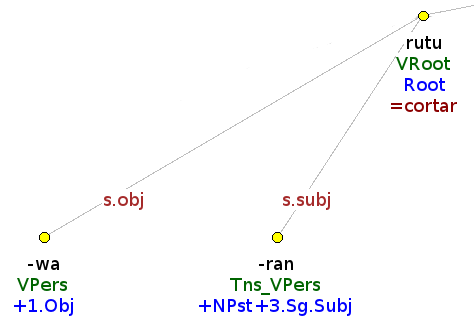
\includegraphics[scale=.4]{verbRoot.png}
%  \end{minipage}
% \begin{minipage}{0.5\textwidth}
%   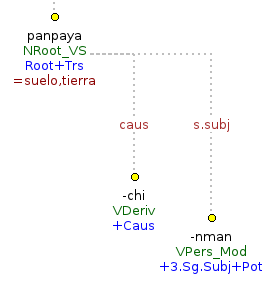
\includegraphics[width=5cm]{verbRoot2.png}
% \end{minipage}}
\begin{center}\fbox{
\begin{tikzpicture}
   
  \draw (0,0) node (chayamu) {chayamu};
      \draw (0,-2) node (-shani) {-shani};
  \draw (5,0) node (panpaya) {panpaya};
  \draw (6,-2) node (-chi) {-chi};
  \draw (8,-2) node (-nman) {-nman};

     \path[-] (-shani) edge  node[label=left:$s.subj$]{} (chayamu);
    \path[-] (-chi) edge  node[label=left:$caus$] {} (panpaya);
     \path[-] (-nman) edge  node[label=right:$s.subj$] {} (panpaya);
\end{tikzpicture}}
\caption{Cabezas en formas verbales}\label{Fig:VRoot}
\end{center}
\end{figure}

  \subsubsection{Ra\'ices nominales verbalizadas}
   Verbalizadores no se consideran un l\'imite de derivaci\'on (derivation boundary), as\'i que la ra\'iz nominal y el sufijo verbalizador constituyen un solo IG. Este se trata como las ra\'ices verbales, descritas en p\'arrafo \ref{Sec:verbRoot}.
  \subsection{Sufijos verbales}
  Hay diferentes clases de sufijos verbales, y la anotaci\'on no es igual para todos.
  \subsubsection{Derivaci\'on}
    Como sufijos de derivaci\'on se entienden aqu\'i los sufijos del Cuadro \ref{Tab:VDeriv}.

\begin{table}
\caption{Sufijos de derivaci\'on verbal}\label{Tab:VDeriv}
\begin{center}
\begin{tabular}{ll}
\toprule
-ymana & +Rem\\
-pasa  & +Desesp\\
-ypari/-rpari & +Int\\
-yqari & +Stat\_Multi\\
-rqari & +Multi\\
-tiya & +Sml\\
-kacha/-ykacha & +Intrup\\
-nya/-miya & +Cont\\
-raya/-nraya & +Perdur\\
-yku/-yu & +Aff\\
-rqu/-ru & +Rptn\\
-ysi/-schi & +Ass\\
-naya & +Des \\
-cha & +Vdim\\
-pa & +Rep\\
-paya & +MRep\\
-na & +Rzpr\\
-chi & +Caus\\
-ri & +Inch\\
-lli & +Autotrs\\
-ku & +Rflx\_Int\\
-mu & +Cis\_Trs\\
-pu & +Rgr\_Iprs\\
\bottomrule
\end{tabular}
\end{center}
\end{table}

Todos estos sufijos, excepto \textit{-ku} y {\em -chi}, no se separan de la ra\'iz verbal, as\'i que no hace falta integrarlos al \'arbol sint\'actico. \\
{\em -ku} y {\em -chi} al contrario se separan de la ra\'iz, los dos sufijos dependen de la ra\'iz con la etiqueta 'mod' (modifier), v\'ease Fig. \ref{Fig:ku}.

\begin{figure}
%  \begin{center}
%  \fbox{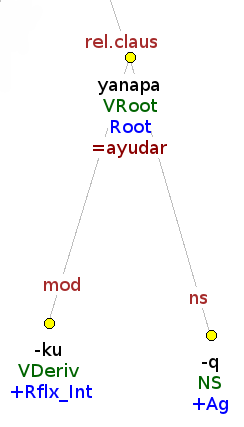
\includegraphics[scale=0.6]{tred7.png}}
% \end{center}
\begin{center}\fbox{
 \begin{tikzpicture}
   \draw (1,1) node (text) {\small{\em yanapakuq}};
     \draw (0,0) node (yanapa) {yanapa};
         \draw (1,-2) node (-ku) {-ku};
         \draw (3,-2) node (-q) {-q};


       \path[-] (-ku) edge  node[label=left:$mod$] {} (yanapa);
       \path[-] (-q) edge  node[label=right:$ns$] {} (yanapa);
\end{tikzpicture}}
\caption{Reflexivo {\em ku}}\label{Fig:ku}
\end{center}
\end{figure}


\subsubsection{Objeto}\label{Sec:objeto}
El siguiente IG contiene los marcadores de 1{\textordfeminine} y 2{\textordfeminine} persona objeto {\em -wa} y {\em -su}. Estos sufijos dependen de la ra\'iz verbal con la etiqueta 's.obj', v\'ease Fig. \ref{Fig:su_wa}.
% 
% \begin{figure}
% \begin{center}
%   \fbox{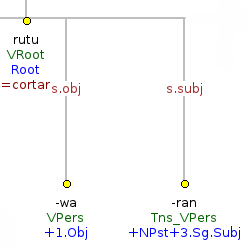
\includegraphics[width=6cm]{tred10.png}}
% \end{center}
% \caption{Marcadores de objeto ({\em -su} y {\em -wa})}\label{Fig:su_wa}
% \end{figure}
\begin{figure}
\begin{center}\fbox{
\begin{tikzpicture}
      \draw (1.5,1) node (text) {\small{\em rutuwaran}};
  \draw (0,0) node (rutu) {rutu};
      \draw (1,-2) node (-wa) {-wa};
  \draw (3,-2) node (-ran) {-ran};
     \path[-] (-wa) edge  node[label=left:$s.obj$]{} (rutu);
     \path[-] (-ran) edge  node[label=right:$s.subj$]  {} (rutu);
\end{tikzpicture}}
 \caption{Marcadores de objeto ({\em -su} y {\em -wa})}\label{Fig:su_wa}
\end{center}
\end{figure}


En el caso de sufijos 'portmanteau' que marcan sujeto y objeto, y que no se dejan separar claramente en una componente de sujeto y otra de objeto, se emplea la etiqueta 's.subj\_obj', v\'ease p\'arrafo \ref{Sec:TAM}.
En verbos ditransitivos se emplea la etiqueta 's.subj\_iobj', v\'ease el ejemplo \ref{Fig:tawan}.

  \subsubsection{TAM y sujeto}\label{Sec:TAM}
El pr\'oximo IG ('inflectional group') consiste del marcador de aspecto {\em -sha}, los marcadores de tiempo {\em -rqa} y {\em -sqa}, el marcador de persona (excepto los marcadores de 1{\textordfeminine} y 2{\textordfeminine} persona objeto, v\'ease \ref{Sec:objeto}), y el marcador {\em -man} del potencial.
El \'unico sufijo que no es opcional en este IG en un verbo finito es el marcador de persona, con una excepci\'on: Con los marcadores de tiempo {\em -rqa} y {\em -sqa}, la marca de de 3{\textordfeminine} persona sujeta {\em -n} puede faltar. En este caso, la etiqueta morfol\'ogica de los sufijos temporales lleva la informaci\'on de persona:
\begin{center}
\begin{tabular}{llll}
\toprule
{\em-sqa} & $\rightarrow$ & +3.Sg.IPst & en vez de: +IPst\\
{\em-rqa} & $\rightarrow$ & +3.Sg.NPst  & en vez de: +NPst\\
\bottomrule
\end{tabular}
\end{center}

En el caso de que este IG contenga s\'olo la persona de sujeto, y no de objeto, depende de la ra\'iz con la etiqueta 's.subj'.\\
En el caso de que el IG contenga un sufijo de persona complejo que no se deja separar claramente en sujeto y objeto, se usa la etiqueta 's.subj\_obj'. Por ejemplo, el sufijo {\em -sunki} '\'el a ti', no se deja separar en una marca de sujeto y objeto, porque morfol\'ogicamente, est\'a marcado dos veces la 2{\textordfeminine} persona. En cambio, la combinaci\'on {\em -wan} '\'el a mi' se deja separar en {\em -wa} '1{\textordfeminine} objeto' y {\em -n} '3{\textordfeminine} sujeto'. En este caso, {\em -wa} recibe la etiqueta 's.obj' y {\em -n} recibe la etiqueta 's.subj'.\\
Notase que en el segundo caso, el IG que contiene el marcador de sujeto puede contener tambi\'en sufijos de aspecto, tiempo o modalidad. Aquellos no influyen la anotaci\'on sint\'actica, ya que para el \'arbol sint\'actico no son relevantes, considere el ejemplo con {\em \~nakawankiman}, v\'ease Fig. \ref{Fig:s.subjobj}.\\
Un caso especial es la combinaci\'on del progresivo {\em -sha} con un nominalizador, ya que el nominalizador es un 'derivation boundary', el progresivo forma un IG s\'olo. En este caso, el progresivo depende de la ra\'iz verbal como 'mod' (modificador).

\begin{figure}
 \fbox{
 \begin{minipage}{0.5\textwidth}
\centering
 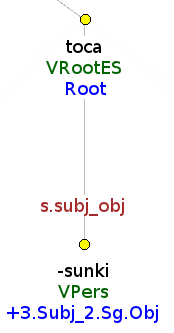
\includegraphics[scale=0.6]{tred8.png}
\end{minipage}
\hfill
\begin{minipage}{0.5\textwidth}
\centering
   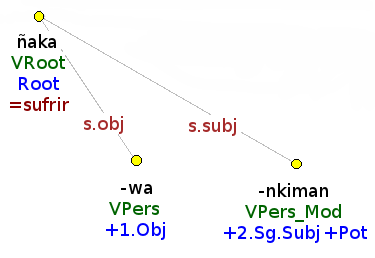
\includegraphics[scale=0.6]{tred9.png}
\end{minipage}}
\caption{Marcadores 'portmanteau' de sujeto y objeto}\label{Fig:s.subjobj}
\end{figure}



  \subsection{Nominalizadores}
Los sufijos nominalizadores son \'estos que se a\~naden a una forma verbal para convertirla en sustantivo, v\'ease el Cuadro \ref{Tab:nominalizadores}.

\begin{table}
\caption{Sufijos nominalizadores}\label{Tab:nominalizadores}
 \begin{center}
\begin{tabular}{ll}
\toprule
-sqa & +Perf\\
-ti & +Char\\
-li & +Char\\
-yli & +Char\\
-liku & +Char\\
-lu & +Char\\
-na & +Obl\\
-q & +Ag\\
-y &  +Inf\\
-mpa & +Posi\\
\bottomrule
\end{tabular}
\end{center}
\end{table}



Estos sufijos dependen de la ra\'iz verbal que nominalizan con la etiqueta 'ns'. Los sufijos nominales que siguen al nominalizador dependen del sufijo nominalizador, no de la ra\'iz verbal, excepto los sufijos de caso: \'estos se anotan como cabeza de la frase entera. V\'ease el ejemplo en Fig. \ref{Fig:NS} de la frase \textit{llank'ana maskhamunaykipaq}: el nominalizador \textit{-na} depende de la ra\'iz como 'ns', y el siguiente sufijo posesivo, que en este caso marca el sujeto, depende del nominalizador. El verbo tiene un objeto, \textit{llank'ana}, que depende de la ra\'iz como 'obj'. La cabeza de la frase entera es el sufijo de caso {\em -paq}.

\begin{figure}
 \fbox{
 \begin{minipage}{0.4\textwidth}
\centering
\vspace{0.2cm}
 {\em \small chayamusqay}\\ \vspace{.3cm}
 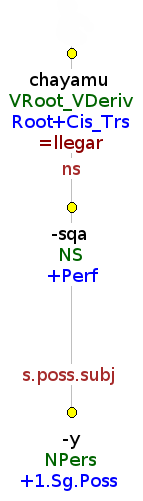
\includegraphics[scale=0.6]{tred11.png}
\end{minipage}
\hfill
\begin{minipage}{0.5\textwidth}
\centering
\vspace{0.2cm}
 {\em \small llank'ana maskhamunaykipaq}\\ \vspace{.3cm}
   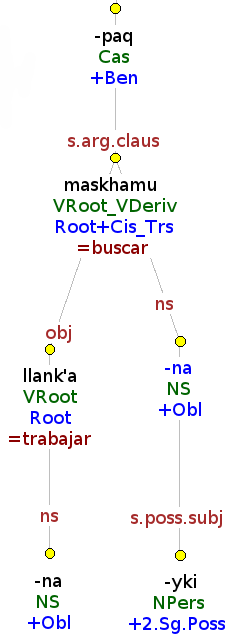
\includegraphics[scale=0.5]{tred12.png}
\end{minipage}}
\caption{Nominalizadores}\label{Fig:NS}
\end{figure}



\section{Sustantivos}
   \subsection{Ra\'ices nominales}\label{Sec:nomroot}
    La ra\'iz nominal es la cabeza del sintagma nominal, con una excepci\'on: si lleva un sufijo de caso, la ra\'iz nominal depende de este sufijo de caso (como 's.arg' o 's.arg.claus' en el caso de verbos nominalizados), descrito en detalle en p\'arrafo \ref{Sec:caso}.
 La ra\'iz nominal puede constituir un IG ('inflectional group') junto con sufijos derivacionales, ya que \'estos no se separan de la ra\'iz.

 \subsubsection{Ra\'ices nominales compuestas}\label{Sec:NRootCMP}
En la combinaci\'on de dos ra\'ices nominales, la primera depende de la segunda como 'mod'. Si las ra\'ices est\'an escritas en una sola palabra ({\em wasimasi}), se separan y la segunda recibe para el atributo 'Tag' ('Morphology') el valor NRootCMP (ra\'iz nominal compuesta).\\
\begin{center}
 \begin{minipage}{0.4\textwidth}
 \begin{examples}
 \item {\em wasi masi} 
 \item {\em unu qucha}
 \item {\em warmi irqi}
\end{examples}
\end{minipage}
\hfill
\begin{minipage}{0.5\textwidth}
\begin{center}\fbox{
\begin{tikzpicture}
      \draw (0,-2) node (wasi) {wasi};
  \draw (1,0) node (masi) {masi};
      \draw (4,-2) node (wasi2) {wasi};
  \draw (5,0) node (-masi) {-masi};
      \draw (5,-0.5) node (NRootCMP) {\small{NRootCMP}};
      \path[-] (masi) edge  node[label=left:$mod$]{} (wasi);
      \path[-] (wasi2) edge  node[label=left:$mod$]  {} (NRootCMP);
\end{tikzpicture}}
% \caption{Ra\'iZ nominal compuesta}\label{Fig:NRootCMP}
\end{center}
%\end{figure}
\end{minipage}
\end{center}


La coordinaci\'on de dos ra\'ices del tipo {\em tayta mama -'padres', tuta p'unchaw - 'd\'ia y noche'} est\'a descrita en p\'arrafo \ref{Sec:coordyuxta}.

\subsubsection{Ra\'ices nominales en funci\'on adjetival}

No hay diferencia entre el uso adjetival de una ra\'iz nominal y las ra\'ices compuestas, descritas en p\'arrafo \ref{Sec:NRootCMP}. La primera ra\'iz, que se usa como adjetivo, depende como 'mod' ('modificador') de la segunda ra\'iz.

\begin{center}
 \begin{minipage}{0.4\textwidth}
 \begin{examples}
 \item {\em hatun allqu}
      'perro grande'
  \item {\em yuraq wasi}
      'casa blanca'
\end{examples}
\end{minipage}
\hfill
\begin{minipage}{0.5\textwidth}
\begin{center}\fbox{
\begin{tikzpicture}
      \draw (0,-2) node (hatun) {hatun};
  \draw (1,0) node (allqu) {allqu};
      \draw (3,-2) node (yuraq) {yuraq};
  \draw (4,0) node (wasi) {wasi};

      \path[-] (hatun) edge  node[label=left:$mod$]{} (allqu);
      \path[-] (yuraq) edge  node[label=left:$mod$]  {} (wasi);
\end{tikzpicture}}
% \caption{Ra\'iZ nominal compuesta}\label{Fig:NRootCMP}
\end{center}
%\end{figure}
\end{minipage}
\end{center}


\subsubsection{Uso adverbial}\label{Sec:adverbios}

Una ra\'iz que modifica un elemento predicativo, depende de \'este como 'adv', v\'ease la anotaci\'on del ejemplo \ref{Ex:adverbios} en Fig. \ref{Fig:adverbios} ('KAN' es un 'dummy element', que se inserta en frases d\'onde la c\'opula (3{\textordfeminine} persona singular) se ha omitido. Ya que anotamos dependencias, necesitamos una cabeza en la frase. Para m\'as informaci\'on acerca de oraciones con c\'opula, v\'ease tambi\'en p\'arrafo \ref{Sec:copula}.) 

\begin{examples}
 \item\label{Ex:adverbios} {\em Payqa \textbf{ancha} munakuq wiraquchan.}\\
      'El es un se\~nor muy amable.'
 \item {\em Maytaq chay \textbf{chika sumaq} ruwasqayki kanasta?}\\
	'{\textquestiondown}D\'onde est\'a esa canasta que has hecho mal?'
 \hfill {\small \citep[116]{Cusi2}}
\end{examples}

\begin{figure}
\begin{center}\fbox{
\begin{tikzpicture}
 \draw  (-1.5,1) node (text) {\em Payqa ancha munakuq wiraquchan};
  \draw (0,0) node (KAN) {KAN};
  \draw (0,-.5) node (DUMMY) {\scriptsize{(DUMMY)}};
  \draw (-1,-2) node (wiraquchan) {wiraquchan};
      \draw (-1,-4) node (munakuq) {munakuq};
      \draw (-1,-6) node (ancha) {\textcolor{blue}{ancha}};
 \draw (-3,-2) node (Payqa) {Payqa};
     \path[-] (Payqa) edge  node[label=left:$subj$]{} (DUMMY);
     \path[-] (wiraquchan) edge  node[label=right:$pred$]  {} (DUMMY);
     \path[-] (munakuq) edge  node[label=right:$mod$]  {} (wiraquchan);
     \path[-,color=blue] (ancha) edge  node[label=right:\textcolor{blue}{$adv$}]  {} (munakuq);
\end{tikzpicture}}
 \caption{Uso adverbial de ra\'ices (\'arbol simplificado)}\label{Fig:adverbios}
\end{center}
\end{figure}


\subsubsection{Reduplicaci\'on}

En el caso de ra\'ices reduplicadas se anota la \'ultima como cabeza, mientras que la primera ra\'iz depende de ella como 'dupl' ('duplicated').

\begin{center}
 \begin{minipage}{0.4\textwidth}
 \begin{examples}
 \item {\em mallki mallki}\\
      'aboleda, bosque, conjunto de \'arboles'
 \item {\em wasi wasi}\\
      'caser\'io, conjunto de casas'
 \item {\em p'unchay p'unchay}\\
      'diario, d\'ia tr\'as  d\'ia'
\end{examples}
\end{minipage}
\hfill
\begin{minipage}{0.5\textwidth}
\begin{center}\fbox{
\begin{tikzpicture}
      \draw (0,-2) node (mallki) {mallki};
  \draw (1,0) node (mallki2) {mallki};
      \draw (3,-2) node (p'unchay) {p'unchay};
  \draw (4,0) node (p'unchay2) {p'unchay};

      \path[-] (mallki) edge  node[label=left:$dupl$]{} (mallki2);
      \path[-] (p'unchay) edge  node[label=left:$dupl$]  {} (p'unchay2);
\end{tikzpicture}}
% \caption{Ra\'iZ nominal compuesta}\label{Fig:NRootCMP}
\end{center}
%\end{figure}
\end{minipage}
\end{center}

   \subsubsection{Verbos nominalizados}
Los nominalizadores dependen de la ra\'iz verbal con la etiqueta 'ns'. Los siguientes sufijos nominales dependen del nominalizador, excepto los sufijos de caso, que son la cabeza de la palabra (v\'ease las figuras \ref{Fig:mantasrc}, \ref{Fig:mantmp} o \ref{Fig:wanco}).

\subsubsection{Pronombres demonstrativos}

Cuando los pronombres demonstrativos sustituyen a un sustantivo (p.e. {\em chayta munani}), se anotan de la misma forma como las ra\'ices nominales (v\'ease p\'arrafo \ref{Sec:nomroot}).\\
Contrario a esto, si los pronombres demonstrativos se usan de forma atributiva (p.e. {\em chay wasita munani}), dependen del sustantivo que modifican y reciben la etiqueta 'det' (determinante, d\'eixis), v\'ease por ejemplo Fig. \ref{Fig:kamamod}.\\
Para la anotaci\'on de un pronombre demonstrativo que resuma una oraci\'on incrustada, v\'ease p\'arrafo \ref{Sec:incrustada}. \\
El uso de pronombres demonstrativos ({\em chayqa, chaymantataq..}) en subordinaciones y coordinaciones est\'a descrito en p\'arrafo \ref{Sec:oraciones}.


\subsection{Sufijos nominales}
  Hay diferentes clases de sufijos nominales, y la anotaci\'on no es igual para todos.
  \subsubsection{Derivaci\'on}
    Como sufijos de derivaci\'on se entienden aqu\'i los sufijos del Cuadro \ref{Tab:NDeriv}.

\begin{table} 
\caption{Sufijos de derivaci\'on nominal}\label{Tab:NDeriv}
\begin{center}
\begin{tabular}{ll}
\toprule
-chika & +Aug\\
-karay & +Aug\\
-chaq & +Aug\\
-chachaq & +Aug\\
-su & +Aug\\
-ti & +Char\\
-li & +Char\\
-yli & +Char\\
-liku & +Char\\
-lu & +Char\\
-cha & +Dim\\
-niray/-niraq & +Sim\\
-rikuq &  +Sim\\
-mpa & +Posi\\ \midrule
-yuq & +Poss\\
-nnaq & +Priv\\
-sapa & +MPoss\\
\bottomrule
\end{tabular}
\end{center}
\end{table}

Los sufijos del primer grupo (sin los tres \'ultimos sufijos en la lista) no se separan de la ra\'iz nominal, sino forman un IG junto con \'esta.\\
En cambio {\em -yuq, -nnaq} y {\em -sapa} se anotan como cabeza del sintagma nominal, la ra\'iz depende de ellos con la etiqueta 's.arg'. La raz\'on es que con {\em -yuq, -nnaq} y {\em -sapa} cambia el referente principal, as\'i p.e. en {\em wasicha, wasiniray, wasimpa} el objeto referido es la casa (o una parte de \'esta), en cambio con {\em wasiyuq}, el referente principal es una persona, no la casa. Por eso, los sufijos {\em -yuq, -nnaq} y {\em -sapa} se consideran la cabeza de la frase nominal. \\
Para la anotaci\'on de {\em -yuq} en n\'umeros, v\'ease p\'arrafo \ref{Sec:numcomplejos}, y para la anotaci\'on de la combinaci\'on {\em ..-yuq + kay} (='tener'), v\'ease p\'arrafo \ref{Sec:yuqkay}.





\subsubsection{Posesivos} Los sufijos posesivos tienen dos anotaciones distintas seg\'un su funci\'on, considere estos ejemplos: {\em wasi\textbf{yki}kuna} vs. {\em rina\textbf{yki}ta munani}. En la primera palabra, el posesivo marca el posesor de un objeto, mientras que en el segundo ejemplo, no se refiere a un posesor, sino al sujeto de un verbo nominalizado. En los dos casos, el sufijo posesivo depende de la ra\'iz, pero la etiqueta de la relaci\'on es distinta: en el primer caso es 's.poss', en el segundo es 's.poss.subj', v\'ease Fig. \ref{Fig:s.poss}.\\

\begin{figure}
 \fbox{ 
\begin{minipage}{0.5\textwidth}
\centering
 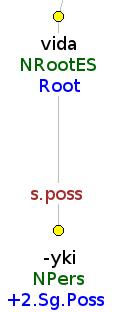
\includegraphics[height=5cm]{tred15.png}
\end{minipage}
\hfill
\begin{minipage}{0.5\textwidth}
\centering
\vspace{0.2cm}
 {\em \small  ..hatunchaña kashaqtiy }\\ \vspace{.3cm}
   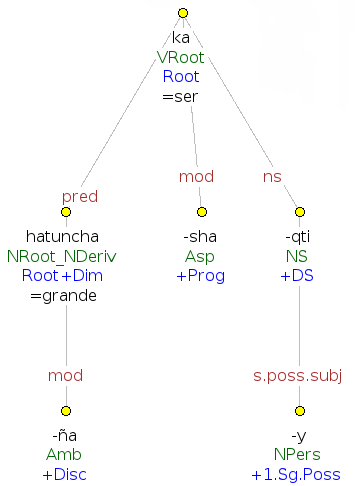
\includegraphics[scale=0.7]{tred36.png}
\end{minipage}}
\caption{Sufijos posesivos}\label{Fig:s.poss}
\end{figure}

El caso no siempre es tan claro, especialmente con infinitivos. Si est\'a absolutamente claro que el sufijo posesivo NO puede entenderse como sujeto, se anota con 's.poss', como en Fig. \ref{Fig:kuna}, en todos los dem\'as casos se anota con 's.poss.subj', como en Fig. \ref{Fig:s.poss.subj}.\\



\begin{figure}
 \begin{center}
  \fbox{
{\parbox{4cm}{
\centering
{\em \small Defensora kaynin..}\\
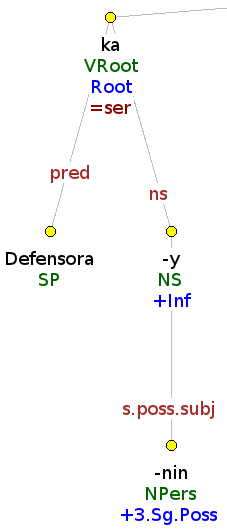
\includegraphics[scale=0.5]{tred16.png}}}}
\end{center}
\caption{Sufijo posesivo como sujeto de verbo nominalizado}\label{Fig:s.poss.subj}
\end{figure}



\subsubsection{Plural}
El sufijo de plural \textit{-kuna} forma parte del IG del morfema que lo precede: En la mayor\'ia de los casos, eso es la ra\'iz, pero tambi\'en puede ser un sufijo de derivaci\'on de posesor ({\em -yuq}) o un sufijo posesivo. En todos casos, {\em -kuna} no recibe una anotaci\'on propia, v\'ease Fig. \ref{Fig:kuna}.

\begin{figure}
 \begin{center}
  \fbox{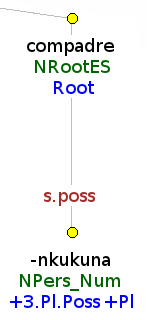
\includegraphics[scale=0.5]{tred17.png}}
\end{center}
\caption{Plural {\em -kuna}}\label{Fig:kuna}
\end{figure}



  \subsubsection{Sufijos de caso}\label{Sec:caso}
Los sufijos de caso siempre se anotan como cabeza del sintagma nominal. Como sufijos de caso se entienden los sufijos del Cuadro \ref{Tab:Caso}.

\begin{table}
\caption{Sufijos de caso}\label{Tab:Caso}
\begin{center}
\begin{tabular}{ll}
\toprule
-nti/-ntin & +Iclsv\\
-pura & +Intsoc\\
-kama & +Distr/+Term\\
-nka & +Distr\\
-niq & +Aprx\\
-ta & +Acc\\
-pa/-p/-q & +Gen\\
-nta & +Proloc\\
-manta & +Abl\\
-man & +Dat\_Ill\\
-paq & +Ben\\
-pi & +Loc\\
-rayku &  +Kaus\\
-wan & +Con\_Inst\\ 
-puwan & +Soc\\
\bottomrule
\end{tabular}
\end{center}
\end{table}

La relaci\'on entre el sufijo de caso y el sintagma nominal que depende de \'el se anota con 's.arg' ('argumento de un sufijo'). La relaci\'on entre el sufijo de caso y su cabeza se anota seg\'un la sem\'antica, puede llevar una de las etiquetas del Cuadro \ref{Tab:CaseLabels}.

\begin{table}
\caption{Etiquetas para sufijos de caso}\label{Tab:CaseLabels}
 \begin{center}
\begin{tabular}{ll}
\toprule
acmp & acompa\~namiento ({\em -ntin})\\
adv & adverbio\\
ben & beneficiario\\
caus & causa ({\em -rayku})\\
co & coordinaci\'on ({\em -wan, -puwan})\\
comp & elemento comparativo ({\em -manta})\\
dir & direcci\'on ({\em -nta})\\
distr & distributivo ({\em -nka, -kama})\\
goal & meta, con verbos de movimiento ({\em -man, -kama, -ta})\\
loc & lugar ({\em -pi, -niq})\\
instr & instrumento ({\em -wan})\\
iobj & objeto indirecto (s\'olo con {\em -man})\\
mod & modificador general\\
obj & objeto (s\'olo con {\em -ta}\\
poss & posesor ({\em -pa})\\
poss.subj & posesor ({\em -pa})\\
purp & fin, objetivo \\
pred & predicativo, s\'olo con c\'opula\\
src & 'or\'igen', con verbos de movimiento ({\em -manta}) \\
sub & subordinaci\'on\\
tmp & modificaci\'on temporal ({\em -pi, -kama..})\\
\bottomrule
\end{tabular}
\end{center}
\end{table}


\paragraph{{\em -ntin}} 
Si expresa acompa\~namiento, se anota con 'acmp', v\'ease la anotaci\'on del ejemplo \ref{Ex:ntin} en Fig. \ref{Fig:ntin}. 

\begin{examples}
 \item\label{Ex:ntin} {\em Chaypi sapallay tiyarani kinsa alqulla\textbf{ntin}}. \\
      'Aquí viví solo, acompañado por tres perros.'\\
           	        \hfill{\small \citep{Valderrama77}}
 \item {\em Mana punchu\textbf{ntin}llanmi hamusqa.}\\	
      'Hab\'ia venido sin poncho.'\\
             	        \hfill{\small \citep[219]{Cusi2}}
\end{examples}

Contrario a esto, el uso de {\em -ntin} para expresar totalidad, se anota seg\'un la funci\'on que tiene en la oraci\'on, por ejemplo:

\begin{examples}
 \item[] 'tmp':
 \item {\em Killa\textbf{ntin}mi Pawkartambopi kamurani.}\\
      'Estuve en Paucartambo todo un mes.'
\item[] 'mod' (modificador de {\em runa}):
 \item {\em Lluy llaqta\textbf{ntin} runa sayarisunchis.}\\
	'Nos pondremos de pie la gente de todo el pueblo.\\
             	        \hfill{\small \citep[219]{Cusi2}}
\end{examples}


\begin{figure}
 \begin{center}
  \fbox{
\parbox{\textwidth}{
\centering 
\vspace{0.3cm}
{\em \small  Chaypi sapallay tiyarani kinsa alqullantin.}\\ \vspace{0.5cm}
{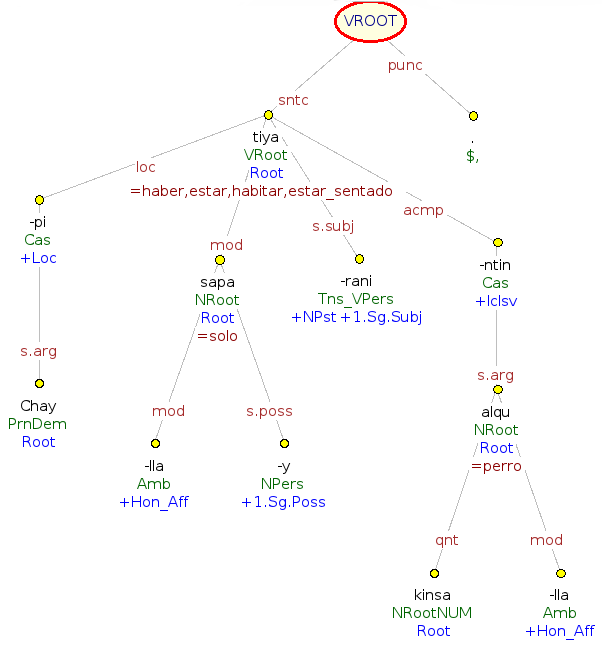
\includegraphics[scale=0.75]{tred18.png}}}}
\end{center}
\caption{Sufijo de caso {\em -ntin}}\label{Fig:ntin}
\end{figure}


\paragraph{{\em -pura}} 
PROVISORIO:
El sufijo {\em -pura}, que indica que cierto n\'umero de seres est\'a entre otros de su misma especie \citep[168]{Soto06}, se anota seg\'un la funci\'on que tiene en la estructura de argumentos del verbo. Si lleva un sufijo de caso m\'as, el \'ultimo sufijo de caso es la cabeza y {\em -pura} depende de 'el como 'mod', como en la anotaci\'on del ejemplo \ref{Ex:puraobj} en Fig. \ref{Fig:puraobj}.\\
V\'ease tambi\'en Fig. \ref{Fig:purasubj} con la anotaci\'on del ejemplo \ref{Ex:purasubj}. 

\begin{examples}
 \item[] sujeto:
 \item\label{Ex:purasubj} {\em Warma\textbf{pura}lla llamkachkanku.} (Ayacuchano)\\
       Trabajan solo entre j\'ovenes.
 \item[] objeto:
 \item\label{Ex:puraobj} {\em Ubihakuna\textbf{pura}llatam taytay munan.} (Ayacuchano)\\
      'Mi padre quiere ovejas nom\'as [no quiere tener tambi\'en chanchos].\\
         	        \hfill{\small \citep[92-95]{Dedenbach02}}
\end{examples}

\begin{figure}
\begin{center}\fbox{
\begin{tikzpicture}
 \draw  (-0,1) node (text) {\em Warmapuralla llamkachkanku (Ayacuchano)};
  \draw (0,0) node (llamka) {llamka};
  \draw (2,-2) node (-chkanku) {-chkanku};
   \draw (-2,-2) node (-pura) {\textcolor{blue}{-pura}};
        \draw (-2,-4) node (warmi) {warmi};
	\draw (-2,-6) node (-lla) {-lla};

     \path[-] (-chkanku) edge  node[label=right:$s.subj$]{} (llamka);
     \path[-] (warmi) edge  node[label=left:$s.arg$]  {} (-pura);
     \path[-] (-lla) edge  node[label=left:$mod$]  {} (warmi);
     \path[-,color=blue] (-pura) edge  node[label=left:\textcolor{blue}{$subj$}]  {} (llamka);
\end{tikzpicture}}
 \caption{Anotaci\'on de {\em -pura} (sujeto)}\label{Fig:purasubj}
\end{center}
\end{figure}

\begin{figure}
\begin{center}\fbox{
\begin{tikzpicture}
 \draw  (-1,1) node (text) {\em Ubihakunapurallatam taytay munan(Ayacuchano)};
  \draw (0,0) node (muna) {muna};
  \draw (2,-2) node (-n) {-n};
   \draw (-1,-2) node (tayta) {tayta};
         \draw (-1,-4) node (-y) {-y};
   \draw (-4,-2) node (-ta) {-ta};
     \draw (-2,-4) node (-pura) {\textcolor{blue}{-pura}};
     \draw (-6,-4) node (Ubihakuna) {Ubihakuna};
	\draw (-6,-6) node (-lla) {-lla};

     \path[-] (-n) edge  node[label=right:$s.subj$]{} (muna);
     \path[-] (Ubihakuna) edge  node[label=left:$s.arg$]  {} (-ta);
     \path[-] (-lla) edge  node[label=left:$mod$]  {} (Ubihakuna);
     \path[-,color=blue] (-pura) edge  node[label=right:\textcolor{blue}{$mod$}]  {} (-ta);
     \path[-] (-ta) edge  node[label=left:$obj$]{} (muna);
     \path[-] (tayta) edge  node[label=right:$subj$]{} (muna);
     \path[-] (-y) edge  node[label=right:$s.poss$]{} (tayta);

\end{tikzpicture}}
 \caption{Anotaci\'on de {\em -pura} (objeto)}\label{Fig:puraobj}
\end{center}
\end{figure}
 
\paragraph{{\em -kama}}

\subparagraph{'mod':} Cuando indica un l\'imite final (de distancia o serie num\'erica) se anota con 'mod'.  
Si se usa en combinaci\'on con {\em -(n)ta}) para denotar una trayectoria o la direcci\'on de un curso, el elemento que determina la relaci\'on con el verbo es {\em -nta}, as\'i que \'este se considera la cabeza. {\em -kama} depende de \'el como 'mod'. V\'ease Fig. \ref{Fig:kamamod} con la anotaci\'on del ejemplo \ref{Ex:kamamod}.\\
PROVISORIO

\begin{examples}
\item {\em Arkipa\textbf{kama}n kay hatun makinaqa rin.}\\
      Este tren grande va hasta Arequipa.
\item {\em Pachak\textbf{kama}llan yupaytaqa yachani.}\\
      S\'e contar s\'olo hasta cien.
\item\label{Ex:kamamod} {\em Kay \~nan\textbf{takama}lla rinki.}\\
      Vaya directamente por este camino.\\
    	 \hfill{\small \citep[130]{Cusi2}}
\end{examples}

\begin{figure}
\begin{center}\fbox{
\begin{tikzpicture}
 \draw  (-1,1) node (text) {\em Kay \~nantakamalla rinki.};
  \draw (0,0) node (ri) {ri};
    \draw (2,-2) node (-nki) {-nki};
    \draw (-2,-2) node (-ta) {-ta};
	\draw (0,-4) node (-kama) {\textcolor{blue}{-kama}};
         \draw (-4,-4) node (nan) {\~nan};  
              \draw (-6,-6) node (Kay) {Kay};
              \draw (-2,-6) node (-lla) {-lla};


     \path[-,color=blue] (-kama) edge  node[label=right:\textcolor{blue}{$mod$}]  {} (-ta);
     \path[-] (-nki) edge  node[label=right:$s.subj$]{} (ri);
     \path[-] (-ta) edge  node[label=left:$mod$]  {} (ri);
     \path[-] (nan) edge  node[label=left:$s.arg$]{} (-ta);
     \path[-] (-lla) edge  node[label=right:$mod$]  {} (nan);
     \path[-] (Kay) edge  node[label=left:$det$]  {} (nan);


\end{tikzpicture}}
 \caption{Anotaci\'on de {\em -kama} (modificador)}\label{Fig:kamamod}
\end{center}
\end{figure}

\subparagraph{'tmp':}
Si {\em -kama} marca un l\'imite temporal, recibe la etiqueta 'tmp'.

\begin{examples}
 \item {\em Yaqa abril\textbf{kama}n paranqa.}\\
      Llover\'a casi hasta el mes de abril.\\
 	 \hfill{\small \citep[129]{Cusi2}}
 \item {\em Wata\textbf{kama}m mana hamunqakuchu.} (Ayacuchano)\\
	'No vendr\'an hasta el pr\'oximo a\~no.'\\
 	        \hfill{\small \citep[81]{Soto76a}}
\end{examples}


\subparagraph{'distr':}\label{Sec:kamadistr}
Cuando {\em -kama} tiene una funci\'on distruibutiva, cuando indica totalidad o repetici\'ones id\'enticas de la acci\'on y se traduce por 'todo(s), cada uno, cada vez, siempre', recibe la etiqueta 'distr'.
En combinaci\'on con otros sufijos de caso, el sufijo que determina la relaci\'on de sustantivo con el resto de la frase es la cabeza.\\
Si {\em -kama} denota el elemento predicativo en una oraci\'on ecuacional, recibe la etiqueta 'pred', v\'ease tambi\'en p\'arrafo \ref{Sec:kayecuacional}.\\
V\'ease Fig. \ref{Fig:kamadistr} con la anotaci\'on del ejemplo \ref{Ex:kamadistr} y Fig. \ref{Fig:kamadistr2} con la anotaci\'on del ejemplo \ref{Ex:kamadistr2}.


\begin{examples}

 \item {\em Allin wasiyuq\textbf{kama}m kay runakunaqa.} (Ayacuchano)\\
      'Estos hombres, cada uno tiene buena casa.'\\
	        \hfill{\small \citep[81]{Soto76a}}

 \item {\em Sapa\textbf{kama} chunka tantata chaskisaqku.} (Ayacuchano)\\
      'Cada uno recibir\'a diez panes.'\\
          \hfill{\small \citep[381]{Soto06}}

  \item\label{Ex:kamadistr} {\em Qhari\textbf{kama}n wawaykunaqa.}\\
	'Todos mis hijos son varones.'
 
  \item\label{Ex:kamadistr2} {\em Hinaspa chay warmi uyapi\textbf{kama} ch'aqlarqarin.}\\
	'Entonces, esa mujer le dio varios sopapos en la cara.'

  \item {\em Mamaypa\textbf{kama}n kay llikllakunaqa.}\\
	Estas mantas son todas de mi mam\'a.\\
  	 \hfill{\small \citep[130]{Cusi2}}
\end{examples}

\begin{figure}
\begin{center}\fbox{
\begin{tikzpicture}
 \draw  (0,1) node (text) {\em Qharikaman wawaykunaqa.};
  \draw (0,0) node (KAN) {KAN};
    \draw (2,-2) node (wawaykuna) {wawaykuna};
         \draw (2,-4) node (-qa) {-qa};
    \draw (-2,-4) node (Qhari) {Qhari};
    \draw (-2,-2) node (-kama) {\textcolor{blue}{-kama}};
     \draw (-2,-2.5) node (FOCUS) {\scriptsize{(FOCUS)}};
         \draw (0,-2) node (-n) {-n};


     \path[-,color=blue] (-kama) edge  node[label=left:\textcolor{blue}{$pred$}]  {} (KAN);
     \path[-] (Qhari) edge  node[label=left:$s.arg$]{} (FOCUS);
     \path[-] (wawaykuna) edge  node[label=right:$subj$]  {} (KAN);
     \path[-] (-n) edge  node[label=left:$ev$]{} (KAN);
     \path[-] (-qa) edge  node[label=right:$topic$]  {} (wawaykuna);


\end{tikzpicture}}
 \caption{Anotaci\'on de {\em -kama} (distributivo, 'pred')}\label{Fig:kamadistr}
\end{center}
\end{figure}
 

\begin{figure}
\begin{center}\fbox{
\begin{tikzpicture}
 \draw  (-2,1) node (text) {\em Hinaspa chay warmi uyapikama ch'aqlarqarin.};
  \draw (0,0) node (ch'aqlarqari) {ch'aqlarqari};
    \draw (2,-2) node (-n) {-n};
    \draw (0,-2) node (-pi) {-pi};
	  \draw (1,-4) node (-kama) {\textcolor{blue}{-kama}};
	  \draw (-1,-4) node (uya) {uya};
    \draw (-2,-2) node (warmi) {warmi};
	  \draw (-2,-4) node (chay) {chay};
    \draw (-5,-2) node (Hina) {Hina};
	  \draw (-5,-4) node (-spa) {-spa};


     \path[-,color=blue] (-kama) edge  node[label=right:\textcolor{blue}{$distr$}]  {} (-pi);
     \path[-] (-pi) edge  node[label=right:$loc$]{} (ch'aqlarqari);
     \path[-] (warmi) edge  node[label=left:$subj$]  {} (ch'aqlarqari);
     \path[-] (chay) edge  node[label=left:$det$]{} (warmi);
     \path[-] (Hina) edge  node[label=left:$linker$]  {} (ch'aqlarqari);
     \path[-] (-spa) edge  node[label=left:$ns$]  {} (Hina);
     \path[-] (-n) edge  node[label=right:$s.subj$]  {} (ch'aqlarqari);
     \path[-] (uya) edge  node[label=left:$s.arg$]  {} (-pi);

\end{tikzpicture}}
 \caption{Anotaci\'on de {\em -kama} (distributivo)}\label{Fig:kamadistr2}
\end{center}
\end{figure}


\subparagraph{'sub':}\label{Sec:kamasub}
El uso de {\em -na} + {\em -kama} para expresar una acci\'on simult\'anea, se anota con la etiqueta 'sub' (subordinaci\'on sin especificar).

\begin{examples}
\item {\em Plasa riru\textbf{na}y\textbf{kama} wawata qhawashanki!}\\
      Mientras yo vaya al mercado, t\'u vas a cuidar al bebe.\\
  	 \hfill{\small \citep[129]{Cusi2}}
\item {\em Sama\textbf{na}y\textbf{kama}m pay pukllakuchkan.} (Ayacuchano)\\
      'Juego mientras descanso.'
\item {\em Pisipay-pisipay ka\textbf{na}y\textbf{kama}m llamkasaq.} (Ayacuchano)\\
      Trabajar\'e hasta estar bien cansado.\\
     	        \hfill{\small \citep[81]{Soto76a}}
\end{examples}

V\'ease tambi\'en la descripci\'on de la subordinaci\'on en p\'arrafo \ref{Sec:subordNom}.

% \begin{figure}
% \begin{center}\fbox{
% \begin{tikzpicture}
%  \draw  (-2,1) node (text) {\em Plasa riru\textbf{na}y\textbf{kama} wawata qhawashanki!};
%   \draw (0,0) node (ch'aqlarqari) {ch'aqlarqari};
%     \draw (2,-2) node (-n) {-n};
%     \draw (0,-2) node (-pi) {-pi};
% 	  \draw (0,-4) node (uya) {uya};
% 	  \draw (0,-6) node (-kama) {\textcolor{blue}{-kama}};
%     \draw (-2,-2) node (warmi) {warmi};
% 	  \draw (-2,-4) node (chay) {chay};
%     \draw (-5,-2) node (Hina) {Hina};
% 	  \draw (-5,-4) node (-spa) {-spa};
% 
% 
%      \path[-,color=blue] (-kama) edge  node[label=right:\textcolor{blue}{$distr$}]  {} (uya);
%      \path[-] (-pi) edge  node[label=right:$loc$]{} (ch'aqlarqari);
%      \path[-] (warmi) edge  node[label=left:$subj$]  {} (ch'aqlarqari);
%      \path[-] (chay) edge  node[label=left:$det$]{} (warmi);
%      \path[-] (Hina) edge  node[label=left:$linker$]  {} (ch'aqlarqari);
%      \path[-] (-spa) edge  node[label=left:$ns$]  {} (Hina);
%      \path[-] (-n) edge  node[label=right:$s.subj$]  {} (ch'aqlarqari);
%      \path[-] (uya) edge  node[label=right:$s.arg$]  {} (-pi);
% 
% \end{tikzpicture}}
%  \caption{Subordinaci\'on con {\em -kama}}\label{Fig:kamasub}
% \end{center}
% \end{figure}

\paragraph{{\em -nka}}
PROVISORIO
\subparagraph{'distr':}  El sufijo {\em -nka} depende de su cabeza como 'distr' (distributivo). El argumento de este sufijo no depende de \'el como 's.arg', sino con la funci\'on que tiene en la oraci\'on (p.e. 'obj').\\
V\'ease Fig. \ref{Fig:nka} con la anotaci\'on del ejemplo \ref{Ex:nka}.

\begin{examples}
 \item {\em Iskay chuqllu\textbf{-nka} haypunki.} (Ayacuchano)\\
      'Repartir\'as dos choclos a cada uno.'\\
              \hfill{\small \citep[381]{Soto06}}
 \item {\em Iskay libru\textbf{nka}s chaskikamusqaku.} (Ayacuchano)\\
      'Dice que recibieron cada uno dos libros.'
 \item\label{Ex:nka} {\em Pachak\textbf{ninka} qusaq.}\\
      'Dar\'e cien a cada uno.'\\
              \hfill{\small \citep[82]{Soto76a}}
\end{examples}


\begin{figure}
\begin{center}\fbox{
\begin{tikzpicture}
 \draw  (-0.2,1) node (text) {\em Pachakninka qusaq.};
  \draw (0,0) node (qu) {qu};
    \draw (2,-2) node (-saq) {-saq};
    \draw (-2,-2) node (-ninka) {\textcolor{blue}{-ninka}};
	  \draw (-2,-4) node (Pachak) {Pachak};



     \path[-,color=blue] (-ninka) edge  node[label=left:\textcolor{blue}{$distr$}]  {} (qu);
     \path[-] (Pachak) edge  node[label=left:$obj$]{} (-ninka);
     \path[-] (-saq) edge  node[label=right:$s.subj$]  {} (qu);
\end{tikzpicture}}
 \caption{Anotaci\'on de {\em -nka}}\label{Fig:nka}
\end{center}
\end{figure}


\paragraph{{\em -niq}} 
\subparagraph{'loc':}
El sufijo {\em -niq} se anota con 'loc' (location) cu\'ando especifica una relaci\'on espacial, o sea, indica la ubicaci\'on aproximada a alg\'un lugar.
\begin{examples}
 \item {kay\textbf{niq}}\\
	un poco m\'as ac\'a
  \item {\em karu\textbf{niq}}\\
	un poco m\'as lejos
  \item {\em may\textbf{niq}}\\
	qu\'e parte m\'as o menos\\
    	 \hfill{\small \citep[220]{Cusi2}}
\end{examples}

\subparagraph{'tmp':} El sufijo {\em -niq} se anota con 'tmp' cuando denota una relaci\'on temporal.

\begin{examples}
 \item {\em qhipa\textbf{niq}}\\
      m\'as posteriormente
 \item {\em tayri\textbf{niq}}\\
      cerca al atardecer\\
    	 \hfill{\small \citep[220]{Cusi2}}
\end{examples}


\paragraph{{\em -ta}}
\subparagraph{'obj':} Si {\em -ta} marca un objeto directo, depende del verbo como 'obj', v\'ease la anotaci\'on para el ejemplo \ref{Ex:taobj} en Fig. \ref{Fig:taobj}.

\begin{examples}
 \item\label{Ex:taobj} {\em Paymi chukchay\textbf{ta} rutuwaran..}\\
	'Ella me cortaba el pelo..'
 \item\label{Ex:taclause} {\em ..chayqa manan maki ñiqiypi hap'iy\textbf{ta} atiykimanñachu}\\
      '..ya no podr\'e tenerte en mi poder, manteni\'endote..'\\
    	 \hfill{\small \citep{Valderrama77}}
 \item {\em Chay wawacha\textbf{ta} pu\~nuyachiy!}\\
	'{\textexclamdown}Haz dormir a esa criatura!'\\
    	 \hfill{\small \citep[120]{Cusi2}}
\end{examples}


\begin{figure}
 \begin{center}
   \fbox{
\parbox{11cm}{
\centering \vspace{0.5cm}
{\em \small Paymi chukchayta rutuwaran.}\\ \vspace{0.5cm}
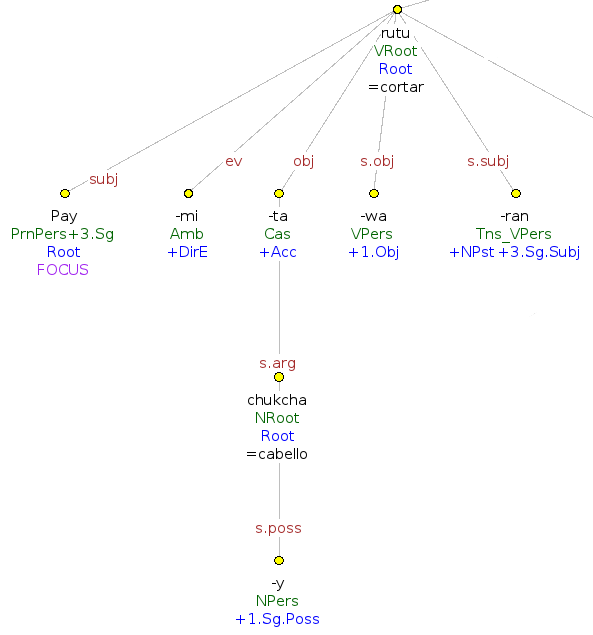
\includegraphics[width=11cm]{tred20.png}}}
\end{center}
\caption{{\em -ta} como marcador de objeto directo}\label{Fig:taobj}
\end{figure}


La anotaci\'on es igual si el 'objeto' es una oraci\'on subordinada de complemento directo, como en el ejemplo \ref{Ex:taclause}, pero el argumento dependiente de {\em -ta} en este caso recibe la etiqueta 's.arg.claus', v\'ease Fig. \ref{Fig:taclause}.

\begin{figure}
 \begin{center}
   \fbox{
\parbox{\textwidth}{
\centering \vspace{0.5cm}
{\em \small ..chayqa manan maki ñiqiypi hap'iyta atiykimanñachu}\\ \vspace{0.5cm}
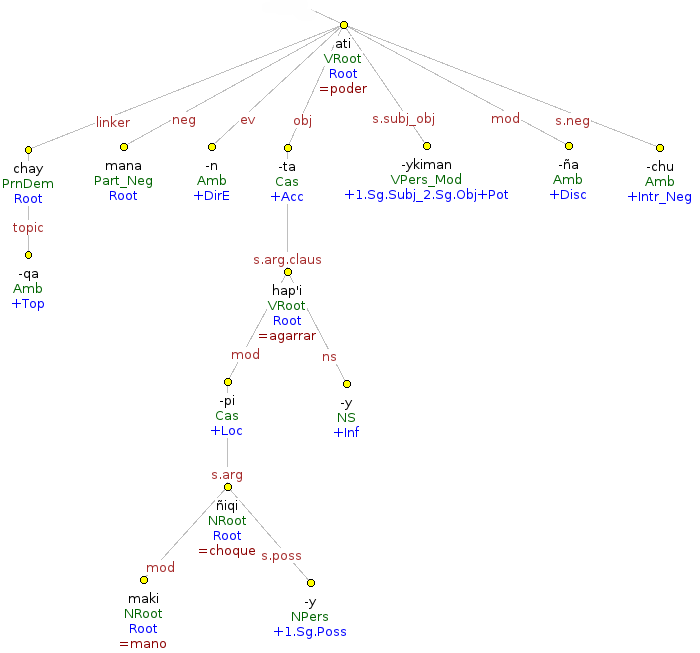
\includegraphics[width=\textwidth]{tred21.png}}}
\end{center}
\caption{{\em -ta} como marcador de una oraci\'on subordinada de complemento directo}\label{Fig:taclause}
\end{figure}

\subparagraph{'adv':} Si {\em -ta} marca una forma adverbial, depende del verbo como 'adv', v\'ease Fig. \ref{Fig:taadverb} con la anotaci\'on del ejemplo \ref{Ex:taadverb}.

\begin{examples}
 \item\label{Ex:taadverb} {\em Allin\textbf{ta}n rishanchis.}\\
      'Estamos yendo bien.'
 \item {\em Sumaq\textbf{ta}n papaqa wi\~namushan.}\\
      'La papa est\'a creciendo muy lindo.'\\
          	 \hfill{\small \citep[121]{Cusi2}}
\end{examples}

\begin{figure}
\begin{center}\fbox{
\begin{tikzpicture}
 \draw  (-1,1) node (text) {\em Allintan rishanchis.};
  \draw (0,0) node (ri) {ri};
    \draw (2,-2) node (-shanchis) {-shanchis};
    \draw (-4,-2) node (-ta) {\textcolor{blue}{-ta}};
	\draw (-4,-2.5) node (FOCUS) {\scriptsize{(FOCUS)}};
	  \draw (-4,-4) node (Allin) {Allin};
    \draw (-2,-2) node (-n) {-n};


     \path[-,color=blue] (-ta) edge  node[label=left:\textcolor{blue}{$adv$}]  {} (ri);
     \path[-] (Allin) edge  node[label=left:$s.arg$]{} (FOCUS);
     \path[-] (-n) edge  node[label=right:$ev$]  {} (ri);
     \path[-] (-shanchis) edge  node[label=right:$s.subj$]  {} (ri);
\end{tikzpicture}}
 \caption{{\em -ta} como marcador adverbial}\label{Fig:taadverb}
\end{center}
\end{figure}

% \begin{figure}
%  \begin{center}
%      \fbox{
% \parbox{4cm}{
% \centering \vspace{0.5cm}
% {\em \small ..allinta atindinayki}\\ \vspace{0.5cm}
% 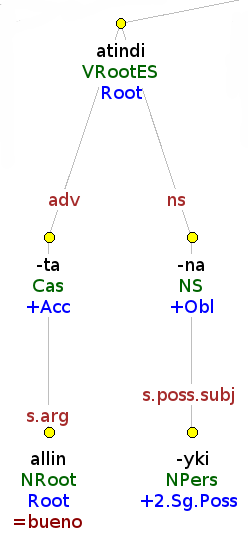
\includegraphics[width=4cm]{tred19.png}}}
% \end{center}
% \caption{{\em -ta} como marcador de un adverbio}\label{Fig:taadverb}
% \end{figure}

\subparagraph{'goal':}
Si {\em -ta} marca al destino de un movimiento, se anota con 'goal', como en el ejemplo \ref{Ex:tagoal} , v\'ease Fig. \ref{Fig:tagoal}.

\begin{examples}
 \item\label{Ex:tagoal} {\em ..huk arriero llaqtayta chayamun..}\\
      '..lleg\'o un arriero a mi pueblo.'\\
    	 \hfill{\small \citep{Valderrama77}}
 \item {\em Nahaqa wasiyki\textbf{ta} hamuranin.}\\
      'Enantes vine a tu casa.'\\
      	 \hfill{\small \citep[122]{Cusi2}}
\end{examples}


\begin{figure}
 \begin{center}
     \fbox{
\parbox{8cm}{
\centering \vspace{0.5cm}
{\em \small ..huk arrierro llaqtayta chayamun..}\\ \vspace{0.5cm}
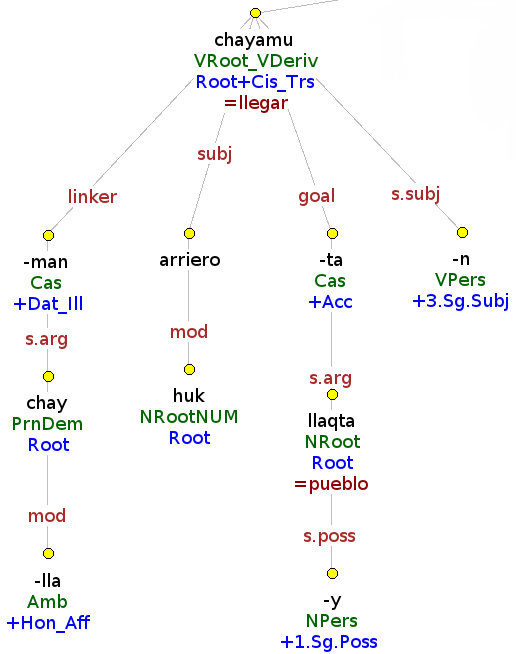
\includegraphics[width=8cm]{tred22.png}}}
\end{center}
\caption{{\em -ta} como marcador de un destino}\label{Fig:tagoal}
\end{figure}

\subparagraph{'tmp' ({\em -ta})}
En algunos casos, {\em -ta} marca a un modificador temporal, v\'ease la anotaci\'on del ejemplo \ref{Ex:tatmp} en Fig. \ref{Fig:tatmp}.

\begin{examples}
 \item\label{Ex:tatmp} {\em  ...chayqa ña tuta\textbf{ta}ña madrinaypa wasinman kutipuni.}\\
	... ya de noche regresé a la casa de mi madrina.\\
	    	 \hfill{\small \citep{Valderrama77}}
\end{examples}

\begin{figure}
 \begin{center}
     \fbox{
\parbox{11cm}{
\centering \vspace{0.5cm}
{\em \small ...chayqa ña tutataña madrinaypa wasinman kutipuni.}\\ \vspace{0.5cm}
{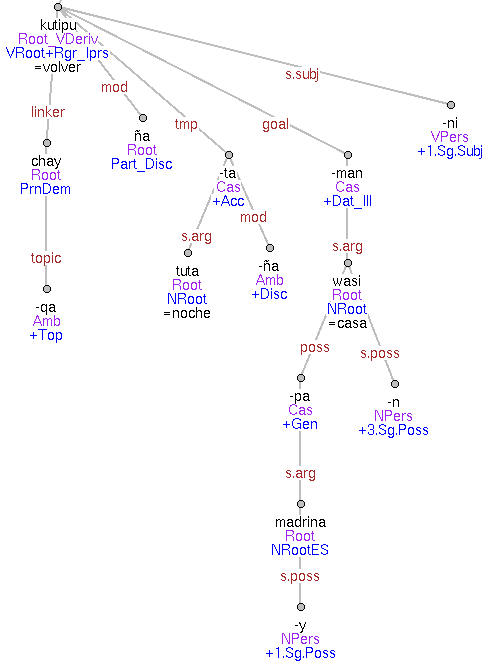
\includegraphics[width=11cm]{tred37.png}}}}
\end{center}
\caption{{\em -ta} como marcador de modificador temporal}\label{Fig:tatmp}
\end{figure}

\subparagraph{'mod' ({\em -nta})}

Para la anotaci\'on de la secuencia {\em -nta} con el significado de 'a trav\'es de, por', v\'ease p\'arrafo \ref{Sec:nta}.


\paragraph{{\em -pa/-p/-q}}
\subparagraph{'poss':} El genitivo {\em -pa} depende del objeto pose\'ido como 'poss', v\'ease la anotaci\'on del ejemplo \ref{Ex:paposesor} en Fig. \ref{Fig:paposesor}.

\begin{examples}
 \item\label{Ex:paposesor} {\em Totalmente q'ara, wakcha madrinay\textbf{pa} makinpi karani.} \\
      'Era totalmente pobre y huérfano y estaba en poder de mi madrina.'\\
    	 \hfill{\small \citep{Valderrama77}}
 \item {\em A\~nas\textbf{pa} t'uqunmi chahayqa.}\\
      'Aquel hueco es la guarida del zorrino.
 \item {\em Rikurankichu wayqiyki\textbf{q} punchunta?}\\
      '{\textquestiondown}Has visto el poncho de tu hermano?'\\
        	 \hfill{\small \citep[129]{Cusi2}}
\end{examples}

\begin{figure}
 \begin{center}\fbox{
  \begin{tikzpicture}
   \draw (-1.5,.5) node (text) {\small{\em ..madrinaypa makinpi karani.}};
  \draw (0,-.5) node (ka) {ka};
      \draw (2,-2) node (-rani) {-rani};
      \draw (-2,-2) node (-pi) {-pi};
	    \draw (-2,-3) node (maki) {maki};
		\draw (0,-4.5) node (-n) {-n};
		\draw (-4,-4.5) node (-pa) {\textcolor{blue}{-pa}};
		\draw (-4,-6) node (madrina) {madrina};
		\draw (-4,-7.5) node (-y) {-y};

    \path[-] (-rani) edge  node[label=right:$s.subj$]{} (ka);
    \path[-] (-pi) edge  node[label=left:$pred$]  {} (ka);
    \path[-,color=blue] (-pa) edge  node[label=left:\textcolor{blue}{$poss$}] {} (maki);
    \path[-] (maki) edge  node[label=left:$s.arg$] {} (-pi);
    \path[-] (-n) edge  node[label=right:$s.poss$] {} (maki);
    \path[-] (-y) edge  node[label=left:$s.poss$] {} (madrina);
    \path[-] (madrina) edge  node[label=left:$s.arg$] {} (-pa);

\end{tikzpicture}}
\caption{{\em -pa} como marcador de posesor}\label{Fig:paposesor}
 \end{center}
\end{figure}


% \begin{figure}
%  \begin{center}
%  \fbox{
% \parbox{4.5cm}{
% \centering \vspace{0.5cm}
% {\em \small madrinaypa makinpi}\\ \vspace{0.5cm}
% 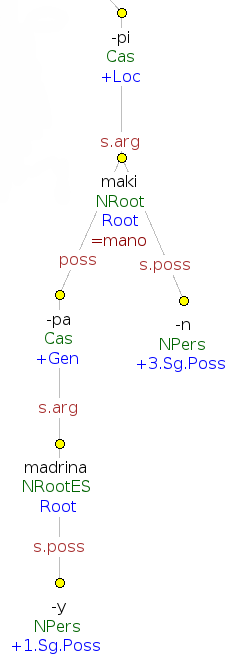
\includegraphics[width=4.5cm]{tred23.png}}}
% \end{center}
% \caption{{\em -pa} como marcador del posesor}\label{Fig:paposesor}
% \end{figure}

\subparagraph{'poss.subj':} Si el genitivo marca el sujeto de un verbo nominalizado, se anota con 'poss.subj'.
V\'ease tambi\'en Fig. \ref{Fig:paqpurp} con la anotaci\'on del ejemplo \ref{Ex:posssubj} (es el mismo ejemplo como \ref{Ex:paqpurp}).

\begin{examples}
 \item {\em Chay wasipiqa mana iskay wata hunt'achu kani patronniy\textbf{pa} niwasqan hina.}\\
    Aqu\'i en esta casa, no estuve los dos a\~nos completos, como me hab\'ia dicho mi patr\'on.\\
      	 \hfill{\small \citep{Valderrama77}}
 \item\label{Ex:posssubj} {\em Ventanata kichay wayra\textbf{q} haykurimunanpaq.}\\
	'Abre la ventana para que entre el aire.'
        	 \hfill{\small \citep[210]{Cusi2}}
\end{examples}


\subparagraph{'mod':}
El uso adverbial de combinaciones de {\em -pa} con ra\'ices que denominan partes del cuerpo se anota con 'adv'.

\begin{examples}
 \item {\em Waqtan\textbf{pa} pu\~nuchkan.} (Ayacuchano)\\
      'Est\'a durmiendo de costado.'
\item {\em Sikin\textbf{pa} wichiykun.} \\
      'Se cay\'o de trasero.'\\
      	 \hfill{\small \citep[78]{Soto76a}}
\end{examples}


\paragraph{{\em -nta}}\label{Sec:nta}
\subparagraph{'mod':}
Se podr\'ia analizar la secuencia {\em -nta} por {\em -n -ta} (posesivo de 3{\textordfeminine} persona, o relacional, m\'as acusativo), como lo hace \citeauthor[122]{Cusi2} en su gram\'atica. \\
Ya que la combinaci\'on {\em -nta} no es composicional en su significado, se trata como unidad para la anotaci\'on sint\'actica. Adem\'as, obs\'ervese la diferencia entre el uso literal en {\em Iskwila\textbf{-n-ta} richkan} 'va a \textbf{su} escuela', y el uso no-literal en los ejemplos abajo.\\
Por lo tanto, la combinaci\'on {\em -nta}, que resulta en un prolocativo  ('por, transversal'), se anota como unidad y recibe la etiqueta 'mod'. V\'ease Fig. \ref{Fig:nta} con la anotaci\'on del ejemplo \ref{Ex:nta}.

\begin{examples}
 \item {\em May\textbf{ninta}taq kay \~nan rin?} (Ayacuchano)\\
      {\textquestiondown}A d\'onde va este camino?\\
        	 \hfill{\small \citep[48]{Dedenbach02}}
 \item\label{Ex:nta} {\em Wasitan suwa haykurusqa ventana\textbf{nta}.}\\
      'El ladr\'on hab\'ia penetrado en la casa, por la ventana.'
 \item {\em Abankay\textbf{ninta}n carreteraqa rishan Andawaylasmanqa.}\\
      'La carretera a Andahuaylas pasa por Abancay.'\\
        	 \hfill{\small \citep[122]{Cusi2}}
\end{examples}

\begin{figure}
 \begin{center}\fbox{
  \begin{tikzpicture}
   \draw (-1,1) node (text) {\small{\em Wasitan suwa haykurusqa ventananta.}};
  \draw (0,0) node (haykuru) {haykuru};
      \draw (1,-2) node (-sqa) {-sqa(\o)};
      \draw (4,-2) node (-nta) {\textcolor{blue}{-nta}};
	    \draw (4,-4) node (ventana) {ventana};
  \draw (-2,-2) node (suwa) {suwa};
  \draw (-4,-2) node (-n) {-n};

  \draw (-6,-2) node (-ta) {-ta};
      \draw (-6,-2.5) node (FOCUS) {\scriptsize{(FOCUS)}};
      \draw (-6,-4) node (Wasi) {Wasi};

    \path[-] (-sqa) edge  node[label=right:$s.subj$]{} (haykuru);
    \path[-] (ventana) edge  node[label=right:$s.arg$]  {} (-nta);
    \path[-,color=blue] (-nta) edge  node[label=right:\textcolor{blue}{$mod$}] {} (haykuru);
    \path[-] (suwa) edge  node[label=right:$subj$] {} (haykuru);
    \path[-] (-n) edge  node[label=left:$ev$] {} (haykuru);
    \path[-] (-ta) edge  node[label=left:$goal$] {} (haykuru);
    \path[-] (Wasi) edge  node[label=left:$s.arg$] {} (FOCUS);

\end{tikzpicture}}
\caption{La combinaci\'on relacional + acusativo {\em -nta}}\label{Fig:nta}
 \end{center}
\end{figure}


\paragraph{{\em -manta}}
\subparagraph{'src':} Si el ablativo {\em -manta} marca el punto de partida de un movimiento, se anota como 'src' ('source'), v\'ease la anotaci\'on del ejemplo \ref{Ex:mantasrc} en Fig. \ref{Fig:mantasrc}.

\begin{examples}
 \item\label{Ex:mantasrc}  {\em ..llaqtaymanta chayamusqay..}\\
	'Vine de mi pueblo..'\\
      	 \hfill{\small \citep{Valderrama77}}
 \item {\em Ch'iqakupi\textbf{manta}s chahay puka pullira sipasqa.}\\
	'Dice que aquella joven de falda colorada es de Checcacupe.'\\
      	 \hfill{\small \citep[125]{Cusi2}}
\end{examples}


\begin{figure}
 \begin{center}
     \fbox{
\parbox{4cm}{
\centering \vspace{0.5cm}
{\em \small ..llaqtaymanta chayamusqay.}\\ \vspace{0.5cm}
{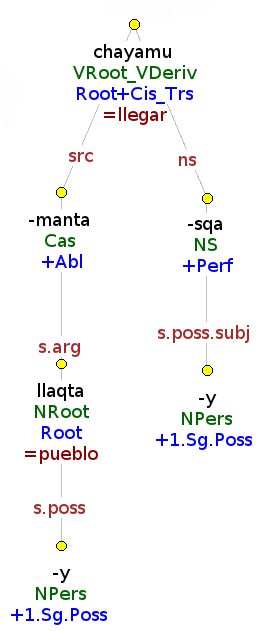
\includegraphics[width=4cm]{tred24.png}}}}
\end{center}
\caption{{\em -manta} como marcador de punto de partida, origen}\label{Fig:mantasrc}
\end{figure}

\subparagraph{'mod':}
PROVISORIO ({\em rimay ..manta} $\rightarrow$ modificador o argumento del verbo?)\\
Si {\em -manta} especifica la materia de una cosa (ejemplo \ref{Ex:mantamateria}), o una caracter\'istica, se anota con 'mod', v\'ease la anotaci\'on del ejemplo \ref{Ex:mantamod} en Fig. \ref{Fig:mantamod}. Si {\em -manta} marca el tema o asunto de lo que se habla, tambi\'en se anota como 'mod'. V\'ease tambi\'en la anotaci\'on de {\em -manta} en Fig. \ref{Fig:nispa2}.

\begin{examples}
 \item\label{Ex:mantamateria} {\em Triyu\textbf{manta}n t'antaqa ruwakun.}\\
      'El pan se hace de trigo.'\\
        	 \hfill{\small \citep[125]{Cusi2}}
 \item\label{Ex:mantamod} {\em ..congresistakuna tukuy niraq partidukuna\textbf{manta}..}\\
      '..congresistas de todos los partidos..'\\
        	 \hfill{\small \citep{Defensora}}
\end{examples}



\begin{figure}
 \begin{center}
     \fbox{
\parbox{8cm}{
\centering \vspace{0.5cm}
{\em \small isqun chunka iskayniyuq congresistakuna tukuy niraq partidukunamanta}\\ \vspace{0.5cm}
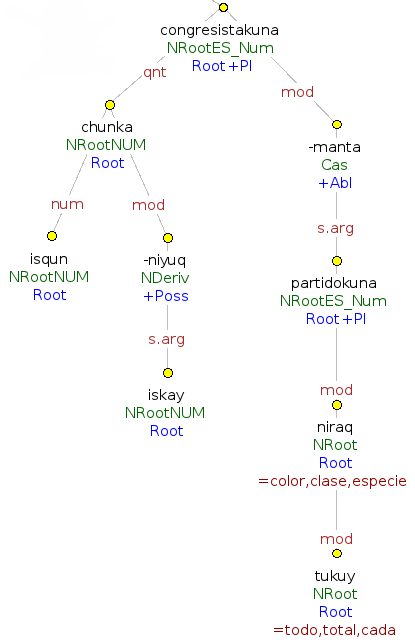
\includegraphics[width=8cm]{tred25.png}}}
\end{center}
\caption{{\em -manta} como marcador de 'materia/caracter\'istica'}\label{Fig:mantamod}
\end{figure}

\subparagraph{'tmp':}
Si {\em -manta} es un modificador 'abtemporal' ('desde'), recibe la etiqueta 'tmp', v\'ease la anotaci\'on del ejemplo \ref{Ex:mantatmp} en Fig. \ref{Fig:mantatmp}. 

\begin{examples}
 \item\label{Ex:mantatmp} {\em 2.003 watapi , junio\textbf{manta} diciembre killakamam Doctora Beatriz Merinoqa , presidenta del Consejo de ministros de la república del Perú nisqa karqa.}\\
    'La Doctora Beatriz Merino era presidenta del Consejo de Ministros de la Rep\'ublica del Per\'u desde junio hasta diciembre del a\~no 2003.\\
          	 \hfill{\small \citep{Defensora}}
\end{examples}


\begin{figure}
 \begin{center}
     \fbox{
\parbox{5cm}{
\centering \vspace{0.5cm}
{\em \small 2.003 wata(pi) junio\textbf{manta} diciembre killakamam}\\ \vspace{0.5cm}
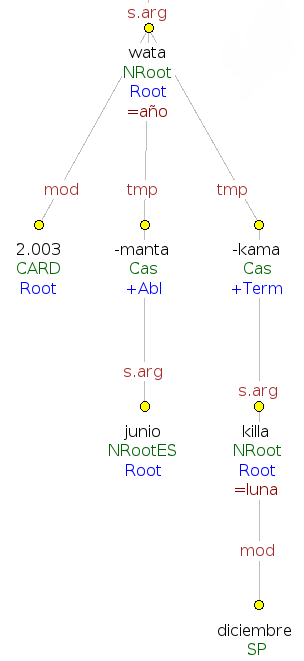
\includegraphics[width=5cm]{tred26.png}}}
\end{center}
\caption{{\em -manta} como marcador abtemporal}\label{Fig:mantatmp}
\end{figure}

\subparagraph{'adv':}
Si {\em -manta} marca a un adverbio, recibe la etiqueta 'adv'.

\begin{examples}
 \item {\em Allillamanta rinkichik.} (Ayacuchano)\\
      'vayan con cuidado'\\
 \hfill {\small \citep[171]{Soto76a}}
\end{examples}

\subparagraph{'comp':}
En construcciones comparativas, {\em -manta} recibe la etiqueta 'comp', v\'ease p\'arrafo \ref{Sec:comparacion}.

\paragraph{{\em -man}} Como argumento del verbo, {\em -man} tiene las siguientes anotaciones:\\

\subparagraph{'iobj':}
 Si {\em -man} marca el objeto indirecto de una oraci\'on ditransitiva, recibe la etiqueta 'iobj' ('indirect object'), v\'ease la anotaci\'on del ejemplo \ref{Ex:maniobj} en Fig. \ref{Fig:maniobj}.

\begin{examples}
 \item\label{Ex:maniobj} \textit{..wintuy\textbf{man}mi aswan kallpata churamusaq,..}\\
	'..a mi viento voy a ponerle más fuerza..'\\
 \hfill {\small \citep{Valderrama77}}
 \item {\em Chahay sipas\textbf{man}si sutiykita willaykunki!}\\
      'Dice que vas a avisar tu nombre a aquella se\'norita.'\\
        	 \hfill{\small \citep[123]{Cusi2}}
\end{examples}


\begin{figure}
 \begin{center}
     \fbox{
\parbox{8cm}{
\centering \vspace{0.5cm}
{\em \small ..wintuymanmi aswan kallpata churamusaq.}\\ \vspace{0.5cm}
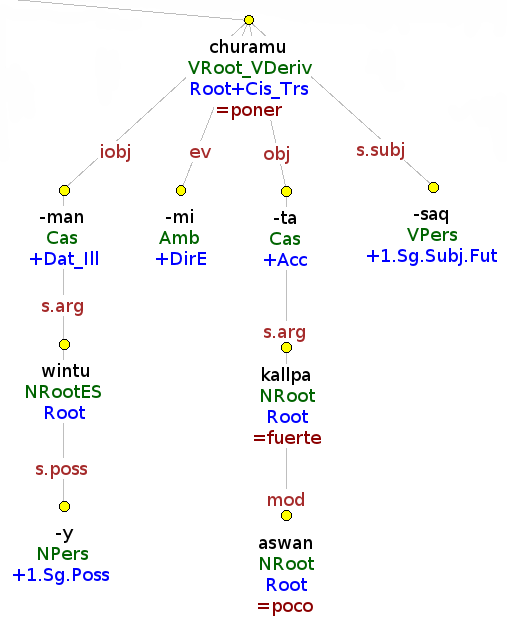
\includegraphics[width=8cm]{tred27.png}}}
\end{center}
\caption{{\em -man} como marcador del objeto indirecto}\label{Fig:maniobj}
\end{figure}


\subparagraph{'arg':}
PROVISORIO (es argumento o es modificador?)POR EL MOMENTO: 'mod'\\
Un caso especial es la combinaci\'on de {\em tukuy ..-man} - 'convertirse a': Aqu\'i {\em -man} no denota un objeto indirecto, ni una meta o direcci\'on, m\'as bien un estado final. Pero no es un simple adjunto ('mod') tampoco, sino un argumento del verbo. Por eso, recibe la etiqueta 'arg', v\'ease Fig. \ref{Fig:manarg}. \\

\begin{figure}
 \begin{center}
     \fbox{
\parbox{6cm}{
\centering \vspace{0.5cm}
{\em \small ..penantemanpas tukuyman.}\\ \vspace{0.5cm}
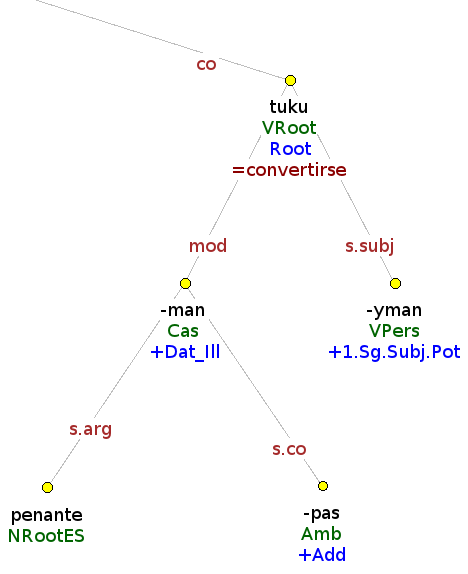
\includegraphics[width=6cm]{tred28.png}}}
\end{center}
\caption{{\em -man} como argumento oblicuo}\label{Fig:manarg}
\end{figure}

\vspace{0.2cm}
Como adjunto, {\em -man} tiene las siguientes anotaciones:\\

\subparagraph{'goal':}
Si {\em -man} indica una meta, o un destino, se anota con 'goal'. Si el adjunto marcado por {\em -man} denota una finalidad, o un objetivo, tambi\'en se anota con 'goal', por ejemplo:


\begin{examples}
 \item {\em May\textbf{man}taq kay \~nanri rishan?}\\
      {\textquestiondown}Y este camino, a d\'onde va?
 \item {\em Urqutan rishani ichhu\textbf{man} panti t'ika\textbf{man} ima.}\\
       Estoy yendo al cerro a traer paja y flores de panti.
 \item\label{Ex:mangoal} {\em Phaway, mamayki\textbf{man} tarparunki.}\\
	{\textexclamdown}Corre, y alcanza tu mam\'a! (tarpay ?)\\
 \hfill {\small \citep[123-124]{Cusi2}}
\end{examples}

 V\'ease Fig. \ref{Fig:mangoal} con la anotaci\'on del ejemplo \ref{Ex:mangoal}.

\begin{figure}
 \begin{center}\fbox{
  \begin{tikzpicture}
   \draw (-1,1) node (text) {\small{\em ..mamayki\textbf{man} tarparunki.}};
  \draw (-0.5,0.5) node (t1) {tarparu};
      \draw (1,-0.7) node (t2) {-nki};
  \draw (-2,-0.7) node (m1) {\textcolor{blue}{-man}};
  \draw (-3,-2) node (m2) {mama};
  \draw (-2.5,-3.5) node (m3) {-yki};

    \path[-] (m3) edge  node[label=right:$s.poss$]{} (m2);
    \path[-] (m2) edge  node[label=left:$s.arg$]  {} (m1);
    \path[-,color=blue] (m1) edge  node[label=left:\textcolor{blue}{$goal$}] {} (t1);
    \path[-] (t2) edge  node[label=right:$s.subj$] {} (t1);
\end{tikzpicture}}
\caption{{\em -man} como marcador de meta o destino}\label{Fig:mangoal}
 \end{center}
\end{figure}



\subparagraph{'tmp':}

Si {\em -man} denota una relaci\'on temporal, recibe la etiqueta 'tmp'.

\begin{examples}
 \item {\em Ch'isi\textbf{man} wasiyta hamunki!}\\
       {\textexclamdown}Vienes a mi casa esta noche!
  \item {\em Wata\textbf{man}qa Arkipatan ripusaq.}\\
	El a\~no que entrante me voy a Arequipa para siempre.\\
 \hfill {\small \citep[124]{Cusi2}}\\
 \item\label{Ex:mantmp} {\em ..(y mana nuqa munanichu) wañusqay qhipa\textbf{man} pipas ñakawananta}\\
	'..y yo no quiero, que despu\'es de mi muerte alguien me maldiga..'\\
 \hfill {\small \citep{Valderrama77}}
\end{examples}



V\'ease la anotaci\'on del ejemplo \ref{Ex:mantmp} en Fig. \ref{Fig:mantmp}.

\begin{figure}
 \begin{center}
   \fbox{
\parbox{8cm}{
\centering \vspace{0.5cm}
{\em \small  ..wañusqay qhipaman pipas ñakawananta.}\\ \vspace{0.5cm}
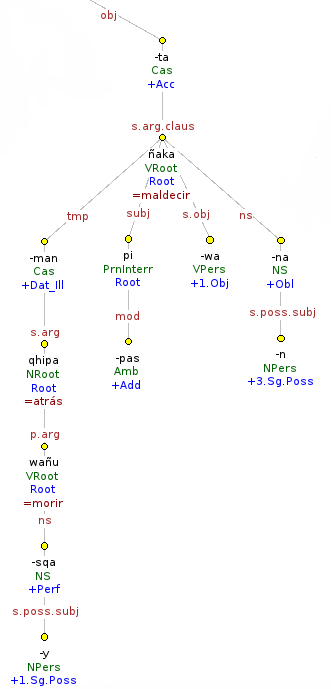
\includegraphics[width=8cm]{tred29.png}}}
\end{center}
\caption{{\em -man} como adjunto temporal}\label{Fig:mantmp}
\end{figure}



\subparagraph{'mod':}
Si {\em -man} no es un argumento del verbo ni se deja categorizar claramente como un adjunto temporal ('tmp') o direccional ('goal'), se anota con 'mod'. 



\paragraph{{\em -paq}}
\subparagraph{'purp':}\label{Sec:paqpurp} En combinaci\'on con el nominalizador {\em -na} el sufijo {\em -paq} denota un fin, un objetivo o una intenci\'on. En este caso, el argumento (=verbo nominalizado) depende de {\em -paq} como 's.arg.claus' (clausal suffix argument), y {\em -paq} depende del verbo de la frase principal como 'purp' (purpose). V\'ease Fig. \ref{Fig:paqpurp} con la anotaci\'on del ejemplo \ref{Ex:paqpurp}.

\begin{examples}
 \item {\em Allin runa kanay\textbf{paq}mi edukakushani.}\\
	Estoy educ\'andome para ser un individuo \'util.\\
	 \hfill{\small \citep[128]{Cusi2}}
 \item\label{Ex:paqpurp} {\em Ventanata kichay wayraq haykurimunanpaq.}\\
      'Abre la ventana para que entre el aire.'\\
	 \hfill{\small \citep[210]{Cusi2}}
\end{examples}

\begin{figure}
 \begin{center}\fbox{
  \begin{tikzpicture}
   \draw (4,1) node (text) {\small{\em Ventanata kichay wayraq haykurimunanpaq.}};
  \draw (0,0) node (kicha) {kicha};
      \draw (1,-2) node (-y) {-y};
  \draw (-2,-2) node (-ta) {-ta};
	\draw (-2,-4) node (Ventana) {Ventana};
  \draw (6,-2) node (-paq) {-paq};
	\draw (6,-4) node (haykurimu) {haykurimu};
	      \draw (4,-6) node (-q) {-q};
		  \draw (4,-8) node (wayra) {wayra};
	      \draw (8,-6) node (-na) {-na};
		  \draw (8,-8) node (-n) {-n};

    \path[-] (-y) edge  node[label=right:$s.subj$] {} (kicha);
    \path[-] (-ta) edge  node[label=left:$obj$] {} (kicha);
	  \path[-] (Ventana) edge  node[label=left:$s.arg$] {} (-ta);
    \path[-,color=blue] (-paq) edge  node[label=right:\textcolor{blue}{$purp$}] {} (kicha);
    \path[-] (haykurimu) edge  node[label=right:$s.arg.claus$]  {} (-paq);
	\path[-] (-na) edge  node[label=right:$ns$]{} (haykurimu);
	    \path[-] (-n) edge  node[label=right:$s.poss.subj$]{} (-na);
	\path[-] (-q) edge  node[label=left:$poss.subj$]{} (haykurimu);
	     \path[-] (wayra) edge  node[label=left:$s.arg$]{} (-q);

\end{tikzpicture}}
\caption{{\em -paq} como marcador de una oraci\'on final}\label{Fig:paqpurp}
 \end{center}
\end{figure}

\subparagraph{'mod'} 
Cuando {\em -paq} denota una acci\'on, un evento que va a pasar en un futuro muy cercano, se anota con 'mod' (ejemplo \ref{Ex:paqmod1}). De la misma forma recibe la etiqueta 'mod' cu\'ando se deja traducir como 'a cambio de', como en ejemplo \ref{Ex:paqmod2}.

\begin{examples}
 \item \label{Ex:paqmod1} {\em Paray\textbf{paq} kachkan.} (Ayacuchano)\\
	 'Est\'a por llover.' \\
	 \hfill{\small \citep[64]{Dedenbach02}}
  \item \label{Ex:paqmod2} {\em Papay\textbf{paq} quwankimanchu chay saraykita?}\\
	 '{\textquestiondown}Puedes darme tu ma\'iz a cambio de mis papas?' \\
	 \hfill{\small \citep[128]{Cusi2}}
\end{examples}

\subparagraph{'ben':} 
Si {\em -paq} marca al beneficiario de una acci\'on o una circunstancia, se anota con 'ben'.
\begin{examples}
 \item {\em Pi\textbf{paq}taq chay punchutari awashanki?}\\
	{\textquestiondown}Para qui\'en est\'as tejiendo ese poncho?\\
	 \hfill{\small \citep[127]{Cusi2}}
\end{examples}


\paragraph{{\em -pi}}\label{Sec:pi}
\subparagraph{'loc':} Cuando {\em -pi} denota un adjunto locativo, recibe la etiqueta 'loc'. 
\begin{examples}
 \item {\em Umayki\textbf{pi} chay yachasqaykita allinta hap'iy.}\\
	Asimila bien en tu cerebro eso que has aprendido.
  \item {\em Ayakuchu\textbf{pi}pas Wankayo\textbf{pi}pas runasimitaqa rimankun.}\\
	Tambi\'en se habla Quechua en Ayacucho y Huancayo.\\
 \hfill {\small \citep[125]{Cusi2}}
\end{examples}

V\'ease tambi\'en Fig. \ref{Fig:kamadistr2} como ejemplo (combinaci\'on de {\em -pi} y {\em -kama}).


\subparagraph{'sub':}\label{Sec:pisub} Cuando {\em -pi} se combina son una forma nominal de un verbo en {\em -sqa} o {\em -na}, para describir una acci\'on paralela o la circunstancia de un evento, recibe la etiqueta 'sub'. 
\begin{examples}
 \item\label{Ex:pisub} {\em Huq kutinkunapiqa uwiha michiq risqay\textbf{pi} , pukllasqay\textbf{pi} puñurapuq kani, chaykamataq uwihakuna dañorukuq kanku.} \\
Otras veces cuando iba a pastear las ovejas, jugando, me quedaba dormido y mientras, las ovejas se dañaban [..]\\
 \hfill {\small \citep{Valderrama77}}
\end{examples}

V\'ease la anotaci\'on del ejemplo \ref{Ex:pisub} en Fig. \ref{Fig:pisub}.


\begin{figure}
 \begin{center}
     \fbox{
\parbox{15cm}{
\centering 
\vspace{0.3cm}
{\em \small ..Huq kutinkunapiqa uwiha michiq risqay\textbf{pi}, pukllasqay\textbf{pi} puñurapuq kani..}\\ \vspace{0.5cm}
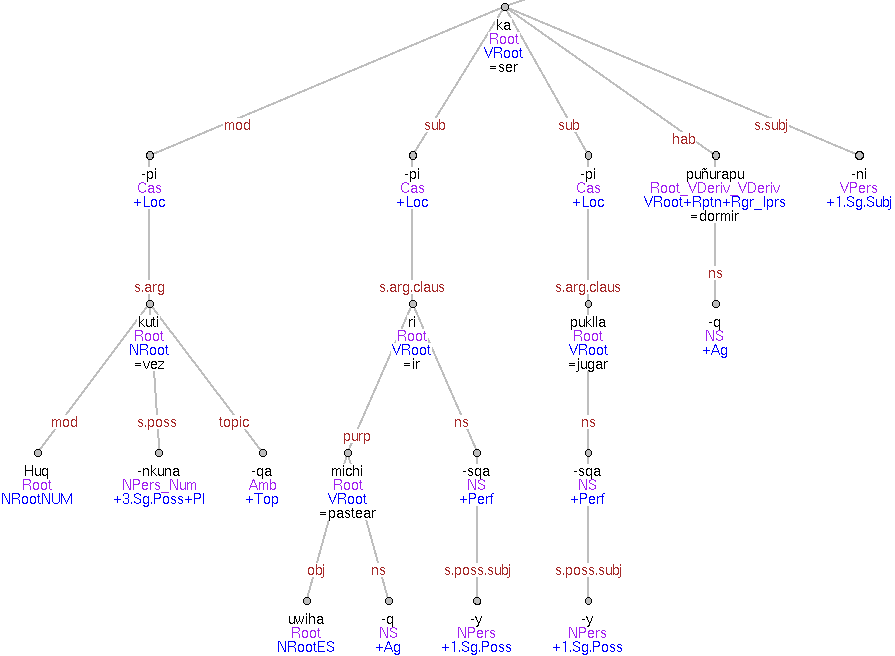
\includegraphics[width=15cm]{tred38.png}}}
\end{center}
\caption{{\em -pi} con oraci\'on subordinada}\label{Fig:pisub}
\end{figure}


\subparagraph{'mod':}
Cuando {\em -pi} denota un medio de transporte, o una circunstancia de una acci\'on, se anota con 'mod', v\'ease la anotaci\'on del ejemplo \ref{Ex:pimod} en Fig. \ref{Fig:pimod}.
\begin{examples}
 \item\label{Ex:pimod} {\em Chakilla\textbf{pi}n eskuylataqa ripuni.}\\
	A la escuela siempre me voy a pie.\\
 \hfill {\small \citep[125]{Cusi2}}
  \item {\em Kallpay\textbf{pi}qa llallin.}\\
	Corriendo gana.\\
 \hfill {\small \citep[43]{Dedenbach02}}
\end{examples}

\begin{figure}
 \begin{center}\fbox{
  \begin{tikzpicture}
   \draw (-3,1) node (text) {\small{\em Chakillapin eskuylataqa ripuni.}};
  \draw (0,0) node (ripu) {ripu};
      \draw (1,-2) node (-ni) {-ni};
  \draw (-2,-2) node (-ta) {-ta};
	\draw (-2,-4) node (eskuyla) {eskuyla};
	\draw (-2,-6) node (-qa) {-qa};
  \draw (-4,-2) node (-n) {-n};
  \draw (-6,-2) node (-pi) {\textcolor{blue}{-pi}};
  \draw (-6,-2.5) node (FOCUS) {\scriptsize(FOCUS)};
	\draw (-6,-4) node (Chaki) {Chaki};
	      \draw (-6,-6) node (-lla) {-lla};

     \path[-] (-ni) edge  node[label=right:$s.subj$] {} (ripu);
     \path[-] (-ta) edge  node[label=left:$goal$] {} (ripu);
 	  \path[-] (eskuyla) edge  node[label=left:$s.arg$] {} (-ta);
	      \path[-] (-qa) edge  node[label=left:$topic$] {} (eskuyla);
    \path[-,color=blue] (-pi) edge  node[label=above:\textcolor{blue}{$mod$}] {} (ripu);
	\path[-] (Chaki) edge  node[label=left:$s.arg$]  {} (FOCUS);
 	\path[-] (-lla) edge  node[label=right:$mod$]{} (Chaki);
    \path[-] (-n) edge  node[label=left:$ev$]{} (ripu);


\end{tikzpicture}}
\caption{{\em -pi} como modificador}\label{Fig:pimod}
 \end{center}
\end{figure}

\subparagraph{'tmp':}
Si {\em -pi} se usa de una forma temporal, recibe la etiqueta 'tmp', por ejemplo 'septiembre killapi' o '2003 watapi', ve\'ase el ejemplo \ref{Fig:mantatmp}.


\paragraph{{\em -rayku}}

\subparagraph{'caus':} El sufijo {\em -rayku} se anota con 'caus' ('causa', no tiene nada que ver con el causativo), cuando denota la raz\'on, la causa o justificaci\'on de una acci\'on. V\'ease la anotaci\'on del ejemplo \ref{Ex:raykucaus} en Fig. \ref{Fig:raykucaus}.

\begin{examples}
 \item\label{Ex:raykucaus}{\em Ima\textbf{rayku}taq llank'anchis?}\\
	{\textexclamdown}Por qu\'e trabajamos nosotros?
  \item {\em Waway\textbf{rayku}n noqaqa llank'aq purini.}\\
      Ando buscando trabajo, por mis hijos.
 \hfill {\small \citep[131]{Cusi2}}
\end{examples}

\begin{figure}
 \begin{center}\fbox{
  \begin{tikzpicture}
   \draw (-1.5,1) node (text) {\small{\em Imaraykutaq llank'anchis?}};
  \draw (0,0) node (llank'a) {llank'a};
      \draw (1,-2) node (-nchis) {-nchis};
  \draw (-4,-2) node (-rayku) {\textcolor{blue}{-rayku}};
	\draw (-4,-4) node (Ima) {Ima};
  \draw (-1,-2) node (-taq) {-taq};

    \path[-,color=blue] (-rayku) edge  node[label=above:\textcolor{blue}{$caus$}] {} (llank'a);
     \path[-] (-nchis) edge  node[label=right:$s.subj$] {} (llank'a);
     \path[-] (Ima) edge  node[label=left:$s.arg$] {} (-rayku);
      \path[-] (-taq) edge  node[label=left:$intr$] {} (llank'a);


\end{tikzpicture}}
\caption{{\em -rayku} como adjunto 'causal' }\label{Fig:raykucaus}
 \end{center}
\end{figure}

\subparagraph{'purp':}\label{Sec:raykupurp}
PROVISORIO (de verdad una oraci\'on final..?)\\
Cuando {\em -rayku} se emplea en frases subordinadas en combinaci\'on con {\em -na}, recibe la etiqueta 'purp', ya que esto resulta en una oraci\'on final.

\begin{examples}
 \item {\em Yanapariwa\textbf{na}yki\textbf{rayku}qa ma\~nayusqaykiy\'a asnuyta.}\\
      Te prestar\'e, pues, mi burro con la condici\'on de que me ayudes en otras veces.
 \item {\em Macha\textbf{na}yki\textbf{rayku}ch\'a ahawasillataqa atipakunki!}\\
      {\textexclamdown}Claro que t\'u siempre frecuentas la chicher\'ia a fin de emborracharte!\\
 \hfill {\small \citep[131]{Cusi2}}
\end{examples}



\paragraph{{\em -wan/-puwan}}

\subparagraph{'acmp':}
 Si el sufijo {\em -wan/-puwan} marca al acompa\~nante o un elemento 'adicional' se anota con 'acmp'.
\begin{examples}
 \item {\em Nuqa\textbf{puwan}mi tarpuqqa risaqku.}\\
      Tambi\'en yo voy con ellos a sembrar.
  \item {\em Qan\textbf{wan}mi rimayta munani.}\\
      Quiero hablar contigo.
\item {\em Huq wiraquchakuna\textbf{wan}mi llank'ani.}\\
      Yo trabajo con unos se\~nores.\\
 \hfill {\small \citep[126-127]{Cusi2}}
\end{examples}

\begin{figure}
 \begin{center}\fbox{
  \begin{tikzpicture}
   \draw (-2,1) node (text) {\small{\em Huq wiraquchakunawanmi llank'ani.}};
  \draw (0,0) node (llank'a) {llank'a};
      \draw (1,-2) node (-ni) {-ni};
  \draw (-1,-2) node (-mi) {-mi};
  \draw (-4,-2) node (-wan) {\textcolor{blue}{-wan}};
      \draw (-4,-2.5) node (FOCUS) {\scriptsize(FOCUS)};
	\draw (-4,-4) node (wiraquchakuna) {wiraquchakuna};
	    \draw (-4,-6) node (Huq) {Huq};

    \path[-,color=blue] (-wan) edge  node[label=left:\textcolor{blue}{$acmp$}] {} (llank'a);
      \path[-] (-ni) edge  node[label=right:$s.subj$] {} (llank'a);
      \path[-] (wiraquchakuna) edge  node[label=left:$s.arg$] {} (FOCUS);
       \path[-] (-mi) edge  node[label=left:$ev$] {} (llank'a);
       \path[-] (Huq) edge  node[label=left:$mod$] {} (wiraquchakuna);


\end{tikzpicture}}
\caption{{\em -wan} como marcador de 'acompa\~nante' o elemento adicional }\label{Fig:wanacmp}
 \end{center}
\end{figure}

\subparagraph{'instr':}
Si {\em wan} marca al instrumento o medio con \'el que se realiza una acci\'on, recibe la etiqueta 'instr'. V\'ease la anotaci\'on del ejemplo \ref{Ex:waninstr} en Fig. \ref{Fig:waninstr}.

\begin{examples}
 \item {\em \~Nawinchis\textbf{wan}mi qhawanchis, siminchis\textbf{wan}taq rimanchis.}\\
    Miramos con los ojos, y hablamos con la boca.\\
 \hfill {\small \citep[126-127]{Cusi2}}
 \item \label{Ex:waninstr}{\em Ichuq makin\textbf{wan}mi qillqan.} (Ayacuchano)\\
	 Escribe con la mano izquierda.
  	\hfill{\small \citep[79]{Soto76a}}
\end{examples}

\begin{figure}
 \begin{center}\fbox{
  \begin{tikzpicture}
   \draw (-2,1) node (text) {\small{\em Ichuq makinwanmi qillqan.}};
  \draw (0,0) node (qillqa) {qillqa};
      \draw (1,-2) node (-n) {-n};
  \draw (-1,-2) node (-mi) {-mi};
  \draw (-4,-2) node (-wan) {\textcolor{blue}{-wan}};
      \draw (-4,-2.5) node (FOCUS) {\scriptsize(FOCUS)};
	\draw (-4,-4) node (maki) {maki};
	    \draw (-6,-6) node (Ichuq) {Ichuq};
	    \draw (-2,-6) node (-n2) {-n};

    \path[-,color=blue] (-wan) edge  node[label=left:\textcolor{blue}{$instr$}] {} (qillqa);
      \path[-] (-n) edge  node[label=right:$s.subj$] {} (qillqa);
      \path[-] (maki) edge  node[label=left:$s.arg$] {} (FOCUS);
       \path[-] (-mi) edge  node[label=left:$ev$] {} (qillqa);
       \path[-] (Ichuq) edge  node[label=left:$mod$] {} (maki);
       \path[-] (-n2) edge  node[label=right:$s.poss$] {} (maki);

\end{tikzpicture}}
\caption{{\em -wan} como marcador de instrumento }\label{Fig:waninstr}
 \end{center}
\end{figure}

\subparagraph{??:}
PROVISORIO ('mod'? otra etiqueta?)\\
Otro uso de {\em -wan} es la marca del 'causee' en construcciones causativas.
\begin{examples}
 \item {\em Parquchini chakrata Pedro\textbf{wan}}.\\
     'I have the field irrigated by Peter.' (causee)\\
  	\hfill{\small \citep[216]{Adelaar04}}
\end{examples}

\subparagraph{'co':} Si {\em -wan} conecta los elementos de una coordinaci\'on, se anota con 'co', v\'ease la anotaci\'on del ejemplo \ref{Ex:wanco} en Fig. \ref{Fig:wanco}. Ya que coordinaciones carecen de una cabeza, por convenci\'on el \'ultimo elemento de la coordinaci\'on es la cabeza y los primeros elementos coordinados dependen de \'el. Si hay m\'as que dos elementos coordinados, todos dependen del \'ultimo elemento. V\'ease tambi\'en p\'arrafo \ref{Sec:coorddoble} sobre coordinaciones con 'doble' sufijos. Si {\em -wan} en su funci\'on coordinativa se combina con otro sufijo de caso, {\em -wan} depende de este sufijo como 's.co' mientras que el otro sufijo de caso depende del verbo seg\'un la funci\'on que tiene, v\'ease la anotaci\'on del ejemplo \ref{Ex:tawan} en Fig. \ref{Fig:tawan}.


\begin{examples}
 \item\label{Ex:wanco} {\em ..willma\textbf{wan}, ch'uñu\textbf{wan} moraya\textbf{wan} (chhalananpaq)}\\
	'..para que intercambie lana, chu\~no y moraya.'\\
  	\hfill{\small \citep{Valderrama77}}
 \item\label{Ex:tawan}  Kapulita\textbf{wan} durasnuta\textbf{wan} apamusayki.\\
  'Te traer\'e capul\'ies y duraznos.'
	\hfill{\small \citep[142]{Cusi2}}
\end{examples}

\begin{figure}
 \begin{center}\fbox{
  \begin{tikzpicture}
   \draw (-2,1) node (text) {\small{\em Kapulitawan durasnutawan apamusayki.}};
  \draw (0,0) node (apamu) {apamu};
      \draw (2,-2) node (-sayki) {-sayki};
  \draw (-2,-2) node (-ta) {-ta};
      \draw (-2,-4) node (durasnu) {durasnu};
      \draw (0,-4) node (-wan) {\textcolor{blue}{-wan}};
      \draw (-5,-4) node (-ta2) {-ta};
	    \draw (-6,-6) node (Kapuli) {Kapuli};
	    \draw (-4,-6) node (-wan2) {\textcolor{blue}{-wan}};

    \path[-,color=blue] (-wan) edge  node[label=right:\textcolor{blue}{$s.co$}] {} (-ta);
    \path[-,color=blue] (-wan2) edge  node[label=right:\textcolor{blue}{$s.co$}] {} (-ta2);
      \path[-] (Kapuli) edge  node[label=left:$s.arg$] {} (-ta2);
      \path[-] (durasnu) edge  node[label=left:$s.arg$] {} (-ta);
       \path[-] (-ta2) edge  node[label=left:$co$] {} (-ta);
       \path[-] (-ta) edge  node[label=left:$obj$] {} (apamu);
       \path[-] (-sayki) edge  node[label=right:$s.subj\_iobj$] {} (apamu);

\end{tikzpicture}}
\caption{{\em -wan} como sufijo coordinativo en combinaci\'on con otro sufijo de caso}\label{Fig:tawan}
 \end{center}
\end{figure}


\begin{figure}
 \begin{center}
     \fbox{
\parbox{6cm}{
\centering 
\vspace{0.3cm}
{\em \small ..willmawan, ch'uñuwan morayawan}\\ \vspace{0.5cm}
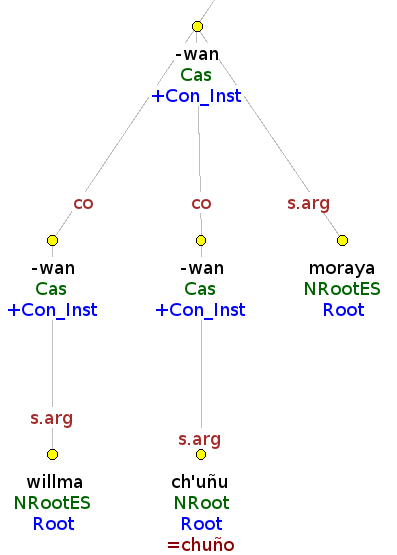
\includegraphics[width=6cm]{tred30.png}}}
\end{center}
\caption{{\em -wan} como coordinador}\label{Fig:wanco}
\end{figure}

\subparagraph{'mod':} Si {\em -wan} no marca al acompa\~nante o al 'causee' o instrumento, ni tiene funci\'on coordinativa, recibe la etiqueta 'mod'.


\subsubsection{Combinaci\'ones de sufijos de caso}

Si un sustantivo lleva m\'as que un sufijo de caso, el sufijo que determina la relaci\'on con el verbo es la cabeza. 
Los dem\'as sufijos de caso dependen de \'el seg\'un su funci\'on, si no tienen una funci\'on espec\'ifica en la frase, se anotan con 's.arg'.
%  Por ejemplo, en la combinaci\'on de {\em -ntakama}, {\em -ta} depende de {\em -kama} como 'obj', mientras que {\em -kama} depende del verbo como 'distr', v\'ease por ejemplo p\'arrafo \ref{Sec:kamadistr}.

\subsubsection{Sufijo de caso como 'elemento predicativo'}

Si una frase marcada por un sufijo de caso en una oraci\'on con copula representa el elemento predicativo, recibe la etiqueta 'pred', v\'ease p\'arrafo \ref{Sec:copula} para m\'as informaci\'on acerca de oraciones con copula.




\section{Sufijos independientes}
 \subsection{{\em -hina,-pacha}}\label{Sec:hinapachasufijos}
En la mayor\'ia de los textos, {\em hina} y {\em pacha} no se escriben como sufijos, adjuntados a la palabra, sino como posposiciones. Pero, ya que algunos autores los escriben como sufijos, hay que definir c\'omo anotarlos en este uso.\\
Los dos sufijos se tratan exactamente igual que las posposiciones {\em hina} y {\em pacha} (v\'ease p\'arrafos \ref{Sec:particulahina} y \ref{Sec:particulapacha}), la \'unica diferencia es que la frase nominal depende de ellos como 's.arg' (argumento de sufijo) en vez 'p.arg' (argumento de posposici\'on).\\ M\'as claro:
 Los sufijos {\em -hina} y {\em -pacha} se anotan como cabeza del elemento que modifican, si es que son ellas que determinan la relaci\'on con la cabeza del elemento (mayormente el verbo);  entonces \'este depende de ellos como 's.arg' (argumento de sufijo) y el sufijo {\em -pacha} recibe la etiqueta 'tmp', mientras que {\em -hina} recibe la etiqueta 'comp'.\\
 PERO: si {\em-hina} se combina con un sufijo de caso, \'este determina la relaci\'on con el verbo, y entonces {\em -hina} depende del sufijo de caso con 'mod'.\\
 TODO: ejemplo





\subsection{{\em -suna/-sina}}
Los sufijos {\em -suna/-sina} siempre dependen de la cabeza de la oraci\'on (mayormente el verbo) como 'epst'. Ya que seg\'un \citeauthor{Cusi2} el sufijo {\em -suna/-sina} tambi\'en marca el foco de la oraci\'on, el atributo 'discourse' el nodo de la cabeza de la palabra que lleva el sufijo {\em -suna/sina} recibe el valor de 'FOCUS', del mismo modo como con los sufijos evidenciales (v\'ease p\'arrafo \ref{Sec:evidenciales}). V\'ease la anotaci\'on del ejemplo \ref{Ex:suna} en Fig. \ref{Fig:suna}.

\begin{examples}
 \item {\em Mana\textbf{suna} ruwasqayqa allinchu.}\\
      'Parece que no est\'a bien lo que estoy haciendo.'
\item\label{Ex:suna} {\em Mamacha\textbf{suna} haqayqa hamush\'an!}\\
      '{\textquestiondown}Creo que es nuestra mamacita aquella que viene?'\\
    		\hfill{\small \citep[235]{Cusi2}}
\end{examples}

\begin{figure}
 \begin{center}\fbox{
  \begin{tikzpicture}
   \draw (-2,1) node (text) {\small{\em Mamachasuna haqayqa hamush\'an!}};
  \draw (0,0) node (hamu) {hamu};
      \draw (1,-2) node (-shan) {-sh\'an};
  \draw (-1,-2.5) node (haqay) {haqay};
      \draw (-1,-4) node (-qa) {-qa};
  \draw (-4,-3) node (-suna) {\textcolor{blue}{-suna}};
  \draw (-7,-2) node (Mamacha) {Mamacha};
      \draw (-7,-2.5) node (FOCUS) {\scriptsize(FOCUS)};

    \path[-,color=blue] (-suna) edge  node[label=left:\textcolor{blue}{$epst$}] {} (hamu);
      \path[-] (-shan) edge  node[label=right:$s.subj$] {} (hamu);
      \path[-] (Mamacha) edge  node[label=above:$l.disl$] {} (hamu);
       \path[-] (haqay) edge  node[label=left:$subj$] {} (hamu);
       \path[-] (-qa) edge  node[label=left:$topic$] {} (haqay);

\end{tikzpicture}}
\caption{Anotaci\'on de {\em -suna}}\label{Fig:suna}
 \end{center}
\end{figure}

  \subsection{{\em-puni}}
PROVISORIO (es necesario distinguir el uso epist\'emico vs. 'siempre'?)
  \subsubsection{Uso epist\'emico}
Si el sufijo {\em -puni} se usa de forma epist\'emica ('ciertamente, definitivamente, necesariamente') depende de la cabeza de la oraci\'on como 'epst'.

\begin{examples}
 \item {\em Mana\textbf{puni}m} (Ayacuchano)\\
      'de ninguna manera'
 \item {\em Warmawan\textbf{puni}m rinki.} (Ayacuchano)\\
      'necesariamente ir\'as con el ni\~no'\\
    		\hfill{\small \citep[128]{Soto76a}}
\end{examples}

\subsubsection{Uso 'habitual' y uso con personas}
Si el sufijo {\em -puni} se usa de forma 'habitual' ('siempre, de costumbre, usualmente') depende de la cabeza de la palabra a la cu\'al est\'a a\~nadido como 'mod'. (TODO: hace sentido distinguir el uso 'siempre' del uso epist\'emico o ser\'a mejor tratarlo igual?)\\
Si {\em -puni} se usa con personas y se traduce como 'mismo', se anota de la misma forma.

\begin{examples}
 \item {\em Mayu killapiqa qasamun\textbf{puni}n.}\\
	'En mayo siempre cae helada.'
 \item {\em Qan\textbf{puni}y\'a riki churachikuranki!}\\
	'Seguramente t\'u mismo te has hecho designar'\\
      		\hfill{\small \citep[244]{Cusi2}}
\end{examples}


 \subsection{{\em-pas/-pis}}
\subsubsection{Adici\'on}
 El sufijo {\em -pas/-pis} en sentido de 'tambi\'en' depende de su ra\'iz como 's.co', v\'ease por ejemplo Fig. \ref{Fig:s.poss} o \ref{Fig:manarg}.
\subsubsection{Coordinaci\'on}
Coordinaciones con dos o m\'as sufijos {\em -pas/-pis} est\'an descritas en p\'arrafo \ref{Sec:coorddoble}.
 \subsubsection{Sustantivos indefinidos}
 PROVISORIO (mejor 'indf'?) \\
Si el sufijo {\em -pas/-pis} se a\~nade a un pronombre interrogativo para formar un 'pronombre indefinido', recibe la etiqueta 'mod'.
\begin{examples}
 \item {\em pipas} - alguien
  \item {\em imapis} - algo
 \item {\em maypis} - alguna parte
\item {\em hayk'aqpas} - alg\'un d\'ia, alguna vez
\end{examples}

V\'ease Fig. \ref{Fig:mananarrow} para la anotaci\'on de {\em pipas}.
\subsubsection{Uso epist\'emico}
PROVISORIO (mejor 'mod'? se puede usar {\em -pas} as\'i sin que {\em -cha} o {\em -chus} lo acompa\~ne?)\\
Si {\em -pas/-pis} se usa de forma epist\'emica, recibe la etiqueta 'epst' y depende de la cabeza de la oraci\'on (mayormente el verbo). 

\begin{examples}
 \item {\em Papataqa qasarapun\textbf{pas}ch\'a!}\\
       '{\textexclamdown}Quiz\'as lo habr\'a helado a las papas!'
 \item tambi\'en en preguntas:\\
      {\em Imatas ch'isiqa musqhukusqani\textbf{p\'as}?}\\
      '{\textquestiondown}No s\'e qu\'e me so\~n\'e anoche?'\\
  		\hfill{\small \citep[239]{Cusi2}}
\end{examples}

\subsubsection{'aunque sea'}

Si {\em -pas/-pis} se usa en el sentido de 'aunque sea', depende de la palabra que modifica como 'mod'.

\begin{examples}
 \item {\em Haku\textbf{pas}y\'a!}\\
      '{\textexclamdown}Aunque sea vamos, pues!'
  \item {\em Ama\textbf{pas} ruwaychuy\'a!}\\
      '{\textexclamdown}Aunque sea no hagas!\\
  		\hfill{\small \citep[240]{Cusi2}}
\end{examples}

\subsubsection{Sugerencias}

Si {\em -pas/-pis} se usa en sugerencias o propuestas como ilustrado por los ejemplos siguientes, depende de la palabra a la cual est\'a adjuntado y recibe la etiqueta 'mod'.

\begin{examples}
 \item {\em Trawutaqa q'u\~niyrachisaqchu [sic] icha kan\textbf{pas}?}\\
      '{\textquestiondown}O quieres que lo haga calentar el licor?'
  \item {\em Mayqintachu munanki\textbf{pas}?}\\
	'{\textquestiondown}O cu\'al quieres?'\\
    		\hfill{\small \citep[239]{Cusi2}}
\end{examples}



  \subsection{{\em-raq/-\~na}}
El sufijo {\em -raq} en todos sus usos depende de 'su' palabra, sea verbal o nominal, como 'mod'.\\
El sufijo {\em \~na} siempre recibe la etiqueta 'mod' tambi\'en, y mayormente depende de 'su' palabra (la palabra a la cu\'al est\'a adjuntado), con una excepci\'on:\\
Si {\em \~na} se usa en combinaci\'on con el sufijo {\em -lla} en el sentido de 'muy, mucho', depende de {\em -lla}, tambi\'en como 'mod'. La combinaci\'on de {\em \~na} y {\em -taq} est\'a descrita en el p\'arrafo \ref{Sec:taqmod}.

\begin{examples}
 \item {\em \~Nan paqarimushan\textbf{\~na}.}\\
	'Ya est\'a amaneciendo el d\'ia'
 \item {\em Haw, haya\textbf{lla\~na}n kay ruqutuqa kasqa.}\\
	'{\textexclamdown}Ay caramba! {\textexclamdown}Este rocoto hab\'ia sido muy picante!'
    		\hfill{\small \citep[246]{Cusi2}}
\end{examples}

V\'ease Fig. \ref{Fig:nia1} y \ref{Fig:nia2} para una ilustraci\'on de los ejemplos.

\begin{figure}
\begin{center}\fbox{
\begin{tikzpicture}[scale=0.9]
   \draw (0,1) node (text) {\small{\em \~Nan paqarimushan\textbf{\~na}.}};
    \draw (-3,-2) node (Na) {\~Na}; 
    \draw (-1,-2) node (-n) {-n}; 
    \draw (0,0) node (paqarimu) {paqarimu};       
  \draw (1,-2) node (-shan) {-shan};
  \draw (4,-2) node (-na) {\textcolor{blue}{-\~na}};
       \path[-] (Na) edge  node[label=left:$mod$] {} (paqarimu);
       \path[-] (-n) edge  node[label=left:$ev$] {} (paqarimu);
       \path[-] (-shan) edge  node[label=right:$s.subj$] {} (paqarimu);
       \path[-,color=blue] (-na) edge  node[label=right:\textcolor{blue}{$mod$}]  {} (paqarimu);

\end{tikzpicture}}
 \caption{Anotaci\'on de {\em  -\~na}}\label{Fig:nia1}
\end{center}
\end{figure}

\begin{figure}
\begin{center}\fbox{
\begin{tikzpicture}[scale=0.9]
   \draw (-1,1) node (text) {\small{\em Haw, haya\textbf{lla\~na}n kay ruqutuqa kasqa.}};
    \draw (0,0) node (ka) {ka}; 
    \draw (0,-2) node (-sqa) {-sqa({\em-\o})}; 
    \draw (-5,-2) node (Haw) {Haw};       
  \draw (-2,-2) node (haya) {haya};
      \draw (-2,-4) node (-lla) {-lla};   
      \draw (-2,-6) node (-na) {\textcolor{blue}{-\~na}};
  \draw (3,-2) node (ruqutu) {ruqutu};
       \draw (3,-4) node (-qa) {-qa};

       \path[-] (-sqa) edge  node[label=right:$s.subj$] {} (ka);
       \path[-] (Haw) edge  node[label=left:$dm$] {} (ka);
       \path[-] (haya) edge  node[label=left:$pred$] {} (ka);
       \path[-] (-lla) edge  node[label=right:$mod$] {} (haya);
       \path[-,color=blue] (-na) edge node[label=right:\textcolor{blue}{$mod$}]  {} (-lla);
	\path[-] (ruqutu) edge  node[label=right:$subj$] {} (ka);
       \path[-] (-qa) edge  node[label=right:$topic$] {} (ruqutu);

\end{tikzpicture}}
 \caption{Anotaci\'on de {\em  -\~na} en combinaci\'on con {\em -lla}}\label{Fig:nia2}
\end{center}
\end{figure}

  \subsection{{\em-taq}}\label{Sec:taq}

\subsubsection{Coordinaci\'on}

Si {\em -taq} se usa en coordinaciones de contraste ('pero, sin embargo, por otra parte'), recibe la etiqueta 's.co' y depende de la palabra a la cu\'al est\'a adjuntado. 

\begin{examples}
 \item {\em Mamayqa qheswatan rin, tatay\textbf{taq} chakrata.}\\
      'Mi mam\'a ha ido a la quebrada, y mi pap\'a a la chacra.'
  \item {\em Hatunmi Piwiray quchaqa, ukhu\textbf{taq} kanpis.}\\
	'La laguna de Piuray es grande, y a la vez honda.\\
  		\hfill{\small \citep[240]{Cusi2}}
\end{examples}

Una descripci\'on de la anotaci\'on de coordinaciones con 'doble' {\em -taq} se encuentra en el p\'arrafo \ref{Sec:coorddoble}.

\subsubsection{Modificador}\label{Sec:taqmod}
El uso de {\em -taq} en exclamaciones de alarma, precauci\'on o amenaza se anota con 'mod', y {\em -taq} depende de la ra\'iz a la cu\'al est\'a a\~nadido. El uso enf\'atico de {\em -taq} que se traduce por 'pues, verdad, ciertamente' tambi\'en se anota as\'i.
\begin{examples}
 \item {\em Waka\textbf{taq} waqrarusunkiman!}\\
      '{\textexclamdown}Cuidado que te cornee la vaca!'
 \item {\em Llaqta masiyi\textbf{t\'aq} kashani, {\textquestiondown}Manachu riqsipuwanki?}\\
      '{\textexclamdown}Soy, pues, tu paisano! {\textquestiondown}No me reconoces?'\\
 		\hfill{\small \citep[241-242]{Cusi2}}
\end{examples}

Un caso un poco m\'as especial es la combinaci\'on de {\em -\~na} y {\em -taq}, para indicar duda o desconfianza acera de la realizaci\'on de la acci\'on \citep[248]{Cusi2}. En este caso, {\em -taq} depende de {\em -\~na} como 'mod', y {\em -\~na} por su parte depende de la ra\'iz como 'mod'.
\begin{examples}
 \item {\em Munanqa\textbf{\~nataq} asnun ma\~nakuyta!}\\
      '{\textexclamdown}Qu\'e va a querer prestarnos su burro!'
\end{examples}

\subsubsection{Preguntas}
Si el sufijo {\em -taq} se usa en preguntas, depende de la cabeza de la oraci\'on (verbo) con la etiqueta 'intr'. 

\begin{examples}
 \item {\em Imata\textbf{taq} ruwashanki?}\\
      '{\textquestiondown}Y qu\'e est\'as haciendo?
  \item {\em Mayta\textbf{taq} qayniwanchayri riranki?}\\
      '{\textquestiondown}Pues, a d\'onde fuiste ayer?'\\
 		\hfill{\small \citep[241]{Cusi2}}
\end{examples}
V\'ease Fig. \ref{Fig:taqintr} para una ilustraci\'on de la anotaci\'on de {\em -taq} en preguntas.

\begin{figure}
\begin{center}\fbox{
\begin{tikzpicture}[scale=0.9]
   \draw (0,1) node (text) {\small{\em Imatataq ruwashanki?}};
    \draw (0,0) node (ruwa) {ruwa}; 
    \draw (2,-2) node (-shanki) {-shanki}; 
    \draw (5,-2) node (-ri) {-ri};       
  \draw (-3,-2) node (-ta) {-ta};
      \draw (-3,-4) node (ima) {ima};   
  \draw (-1,-2) node (-taq) {\textcolor{blue}{-taq}};

       \path[-] (-shanki) edge  node[label=right:$s.subj$] {} (ruwa);
        \path[-] (-ri) edge  node[label=right:$topic$] {} (ruwa);
        \path[-] (-ta) edge  node[label=left:$obj$] {} (ruwa);
       \path[-] (ima) edge  node[label=right:$s.arg$] {} (-ta);
       \path[-,color=blue] (-taq) edge node[label=right:\textcolor{blue}{$intr$}]  {} (ruwa);
\end{tikzpicture}}
 \caption{Uso de {\em -taq} en preguntas}\label{Fig:taqintr}
\end{center}
\end{figure}

\subsection{{\em-chu}}

\subsubsection{Negaci\'on}\label{Sec:chunegacion}
El sufijo {\em -chu} como marcador de negaci\'on depende de la ra\'iz de la palabra a la cu\'al est\'a pegado como 's.neg', v\'ease por ejemplo Fig. \ref{Fig:manawide}, \ref{Fig:mananarrow} y \ref{Fig:manadm}.\\
El sufijo {\em -chu} marca el elemento enfocado de la negaci\'on, por eso, el nodo de la cabeza de la palabra a la cu\'al pertenece {\em -chu} recibe el valor 'FOCUS' para su atributo 'discourse'. Considere estos dos ejemplos:

\begin{examples}
\item {\em Manan huwischu nuqaqa kani.}\\
      'Yo no soy el juez (mi ocupaci\'on es otra).'
\item {\em Manan noqachu huwisqa kani.}\\
     'Yo no soy el juez (el juez es otra persona).'\\
	\hfill{\small \citep[92]{Cusi2}}
\end{examples}



\subsubsection{Preguntas}

El uso interrogativo de {\em -chu} se anota con 'intr', y {\em -chu} depende de la cabeza de la oraci\'on (mayormente el verbo). Ya que {\em -chu} en preguntas tambi\'en marca el foco de la oraci\'on, la cabeza de la palabra a la cu\'al pertenece {\em -chu} recibe el valor de 'FOCUS' para su atributo 'discourse'.\\
Un caso especial son preguntas con dos alternativas marcadas por {\em -chu} y combinadas por {\em icha}. 
Los sufijos {\em -chu} entonces son coordinados (el \'ultimo es la cabeza) y esta coordinaci\'on depende del verbo como 'intr'. Adem\'as, el valor del atributo 'discourse' es 'FOCUS' en la cabeza de la coordinaci\'on con {\em -chu}.


\begin{examples}
 \item {\em Kunan\textbf{chu} icha paqarin\textbf{chu} qarpaqri risunchis?}\\
      '{\textquestiondown}Iremos hoy o ma\~nana a hacer el riego?'
 \item\label{Ex:chu} {\em Paraqayta\textbf{chu} ichari uwinata\textbf{chu} munashanki saratari?}\\
      '{\textquestiondown}Deseas la calidad blanca o la amarilla del ma\'iz?'\\
    		\hfill{\small \citep[236]{Cusi2}}
\end{examples}

V\'ease Fig. \ref{Fig:chucoord} para la anotaci\'on del ejemplo \ref{Ex:chu}. En este caso, el atributo 'discourse' de la coordinaci\'on contiene el valor 'FOCUS'. El elemento {\em saratari} est\'a en la periferia derecha, depende del verbo, pero no como argumento, sino como 'r.disl' ('right dislocution'). V\'ease p\'arrafo \ref{Sec:disl}.

\begin{figure}
\begin{center}\fbox{
\begin{tikzpicture}[scale=0.9]
   \draw (0,3) node (text) {\small{\em Paraqayta\textbf{chu} ichari uwinata\textbf{chu} munashanki saratari?}};
    \draw (0,2) node (muna) {muna}; 
    \draw (4,-2) node (-shanki) {-shanki}; 
    \draw (0,-0.7) node (-chu) {\textcolor{blue}{-chu}};       
  \draw (-3,-2) node (-ta) {-ta};
      \draw (-3,-2.5) node (FOCUS) {\scriptsize(FOCUS)};
  \draw (-6,-2.5) node (-chu2) {\textcolor{blue}{-chu}};
       \draw (-1,-4) node (uwina) {uwina};  
       \draw (-4,-4) node (icha) {icha};  
	  \draw (-4,-6) node (-ri) {-ri};  
       \draw (-7,-4) node (-ta2) {-ta};  
           \draw (-8,-6) node (paraqay) {paraqay};  
    \draw (7,-2) node (-ta3) {-ta}; 
    \draw (7,-4) node (sara) {sara}; 
    \draw (7,-6) node (-ri2) {-ri}; 
 
        \path[-] (-shanki) edge  node[label=right:$s.subj$] {} (muna);
         \path[-,color=blue] (-chu) edge  node[label=right:$intr$] {} (muna);
         \path[-,color=blue] (-chu2) edge  node[label=left:$co$] {} (-chu);
        \path[-] (-ta) edge  node[label=right:$obj$] {} (muna);
        \path[-] (-ta2) edge node[label=right:$co$]  {} (FOCUS);
          \path[-] (paraqay) edge node[label=right:$s.arg$]  {} (-ta2);
          \path[-] (uwina) edge node[label=right:$s.arg$]  {} (FOCUS);
          \path[-] (icha) edge node[label=right:$linker$]  {} (FOCUS);
          \path[-] (-ri) edge node[label=right:$topic$]  {} (icha);

          \path[-] (-ri2) edge node[label=right:$topic$]  {} (sara);
          \path[-] (sara) edge node[label=right:$s.arg$]  {} (-ta3);
          \path[-] (-ta3) edge node[label=right:$r.disl$]  {} (muna);
\end{tikzpicture}}
 \caption{Coordinaci\'on de {\em -chu} en preguntas}\label{Fig:chucoord}
\end{center}
\end{figure}

\subsubsection{Las combinaciones {\em -chu -s} y {\em -chu(s) hina}}

El uso epist\'emico de {\em -chu} en combinaci\'on con el sufijo evidencial {\em -s} est\'a descrito en p\'arrafo \ref{Sec:chus}, y la combinaci\'on de {\em -chu} en combinaci\'on con {\em hina} en p\'arrafo \ref{Sec:chuhina}.

  \subsection{{\em-mi/-si/-cha/-m\'a/-s\'a/ch\'a}}\label{Sec:evidenciales}

Los marcadores de evidencialidad, tambi\'en en sus versiones enf\'aticas ({\em -m\'a, -s\'a, -ch\'a}), dependen de la cabeza de la oraci\'on como 'ev'.
Si el marcador de evidencialidad marca el elemento enfocado de la frase, el atributo de la cabeza de la palabra a la cu\'al pertenece el sufijo {\em -mi/-n/-si/-s/-cha} o {\em -ch} recibe el valor de 'FOCUS'. V\'ease por ejemplo Fig. \ref{Fig:taobj} o  \ref{Fig:aridm}. 
 V\'ease tambi\'en Fig. \ref{Fig:miFOCUS} para la anotaci\'on de {\em chayqa llank'aq\textbf{mi} rinayki.}\\ 

\begin{figure}
\begin{center}
\fbox{
\parbox{7cm}{
\centering \vspace{0.5cm}
{\em \small ..chayqa llank'aqmi rinayki.}\\ \vspace{0.5cm}
 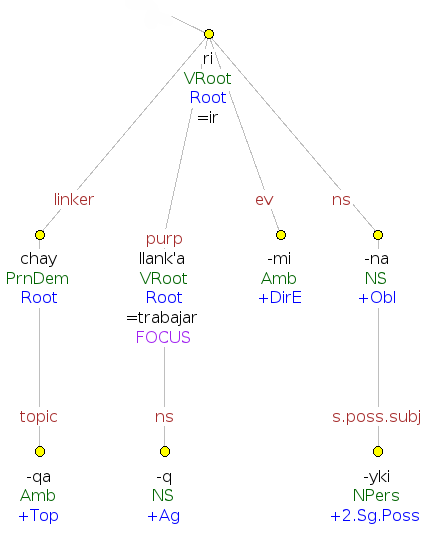
\includegraphics[width=7cm]{tred32.png}}}
 \caption{{\em -mi} como marcador de evidencialidad y foco}\label{Fig:miFOCUS}
\end{center}
\end{figure}

\subsubsection{Evidenciales en negaci\'on}
\begin{examples}
 \item {\em Mana\textbf{m} yuraq wasi\textbf{chu}.} (Ayacuchano)\\
      'No es la casa blanca.'\\
      		\hfill{\small \citep[121]{Soto76a}}
\end{examples}

En negaciones con {\em mana}, el sufijo de evidencialidad normalmente se a\~nade a esta part\'icula, mientras que el sufijo de negaci\'on {\em -chu} marca al elemento enfocado. En este caso, el valor del atributo 'discourse' de la palabra a la cu\'al pertenece el sufijo de evidencialidad es vac\'io, NO es 'FOCUS'. V\'ease tambi\'en el p\'arrafo \ref{Sec:chunegacion} o v\'ease tambi\'en el ejemplo en Fig. \ref{Fig:manadm}.

\subsubsection{Evidenciales en preguntas}
En preguntas que contienen una combinaci\'on de {\em -chu} y un sufijo evidencial, el sufijo evidencial depende del verbo como 'ev'. La cabeza de la palabra a la cu\'al {\em -chu} y el sufijo de evidencialidad pertenecen recibe la anotaci\'on 'FOCUS'.

\begin{examples}
 \item {\em Pay\textbf{chum} tayta Mallma kachkan?} (Ayacuchano)\\
      '{\textquestiondown}Es el se\~nor Mallma?'
 \item {\em Hamunqaku\textbf{chuch} llamkaqkuna?} (Ayacuchano)\\
      '{\textquestiondown}Vendr\'an los trabajadores?\\
    		\hfill{\small \citep[120]{Soto76a}}
\end{examples}

\subsubsection{La combinaci\'on {\em -chu} y {\em -s}}\label{Sec:chus}
La combinaci\'on de {\em -chu} y {\em -s} no tiene una funci\'on evidencial, sino epist\'emica, expresa duda. Por lo tanto, en este caso, el sufijo de evidencial {\em -s} depende de {\em -chu} como 'mod', y {\em -chu} depende de la cabeza de la oraci\'on como 'epst'.

   \subsection{{\em-qa/-ri}}
El marcador de t\'opico {\em -qa} siempre depende de 'su' ra\'iz como 'topic', v\'ease por ejemplo Fig. \ref{Fig:chucoord}.
En cambio, el marcador {\em -ri} tiene dos funciones: marca el t\'opico, pero tambi\'en tiene una funci\'on interrogativa. Por lo tanto, {\em -ri} depende de la cabeza de la oraci\'on (el verbo finito) c\'omo 'intr'.
Con los dos marcadores, el atributo 'discourse' de la cabeza cambia a 'TOPIC'. 


  \subsection{{\em -ya}}
PROVISORIO (o depende del verbo?)\\
El sufijo enf\'atico {\em -ya} depende de la ra\'iz de 'su' palabra como 'mod'.

  
\section{Part\'iculas}
  \subsection{{\em hina}}\label{Sec:particulahina} Si {\em hina} se usa como una posposici\'on, el elemento que {\em hina} modifica depende de la part\'icula como 'p.arg'. {\em hina} mismo depende como 'comp' (si es una comparaci\'on) o como 'mod' de su cabeza. V\'ease \ref{Sec:comparacion} para la anotaci\'on de comparaciones con {\em hina}, y v\'ease \ref{Sec:hinaPP} para la anotaci\'on de {\em hina} como posposici\'on. Para la anotaci\'on del uso epist\'emico de {\em hina} en las combinaciones {\em -chu(s) hina} y {\em hinachu}, v\'ease \ref{Sec:chuhina} y \ref{Sec:hinachu}.

\subsection{{\em pacha} ('desde')}\label{Sec:particulapacha}

En el uso de {\em pacha} como posposici\'on con el significado de 'desde', {\em pacha} constituye la cabeza, la frase nominal depende de {\em pacha} como 'p.arg', mientras que {\em pacha} depende de su cabeza (p.e. el verbo) como  'tmp' (modificador temporal).

  \subsection{{\em mana}} La part\'icula {\em mana} recibe la etiqueta 'neg' de negaci\'on o 'dm', marcador de discurso. 
\subparagraph{'neg':}
Como 'neg' es importante notar que no siempre depende del verbo, qu\'e elemento es su cabeza depende del 'scope' de la negaci\'on.

\begin{examples}
 \item 'narrow scope':\\
	{\em ..pero mana pipas yuyakunchu..}\\
      ..pero nadie se acuerda\\
	v\'ease Fig. \ref{Fig:mananarrow}
 \item  'wide scope':\\
	{\em y mana nuqa munanichu wañusqay qhipaman pipas ñakawananta,..}\\
	..y yo no quiero que después de mi muerte, alguien me maldiga..\\
	v\'ease Fig. \ref{Fig:manawide}\\
 	\hfill{\small \citep{Valderrama77}}	
\end{examples}


\begin{figure}
\begin{center}\fbox{
\begin{tikzpicture}[scale=0.9]
   \draw (4,1) node (text) {\small{\em y mana nuqa munanichu wañusqay qhipaman pipas ñakawananta}};
  \draw (0,0) node (muna) {muna};
    \draw (-2.5,-1.5) node (y) {y};
    \draw (-1.3,-2.5) node (mana) {\textcolor{blue}{mana}};      
    \draw (0.5,-3.5) node (nuqa) {nuqa}; 
    \draw (1.7,-2.5) node (-ni) {-ni}; 
    \draw (3,-1.5) node (-chu) {-chu}; 
    \draw (6,-1.3) node (-ta) {-ta}; 
	     \draw (6,-2.3) node (naka) {\~naka};  
 	     \draw (3.5,-4.3) node (-man) {-man};
		    \draw (3.5,-5.7) node (qhipa) {qhipa};  
		    \draw (3.5,-7.1) node (wanu) {wa\~nu};  
		    \draw (3.5,-8.5) node (-sqa) {-sqa};  
		    \draw (3.5,-9.9) node (-y2) {-y};  
	     \draw (5.5,-4.8) node (pi) {pi};  
		   \draw (5.5,-6.2) node (-pas) {-pas};  
	     \draw (7,-4.3) node (-wa) {-wa}; 
	     \draw (10,-4.3) node (-na) {-na}; 
		  \draw (10,-5.7) node (-n) {-n};  


     \path[-] (y) edge  node[label=left:$linker$]{} (muna);
     \path[-,color=blue] (mana) edge  node[label=left:\textcolor{blue}{$neg$}]  {} (muna);
     \path[-] (nuqa) edge  node[label=$subj$] {} (muna);
     \path[-] (-ni) edge  node[label=right:$s.subj$] {} (muna);
     \path[-] (-chu) edge  node[label=right:$s.neg$] {} (muna);
     \path[-] (-ta) edge  node[label=above:$obj$] {} (muna);

     \path[-] (naka) edge  node[label=right:$s.arg$] {} (-ta);

     \path[-] (-man) edge  node[label=left:$tmp$] {} (naka);
     \path[-] (pi) edge  node[label=left:$subj$] {} (naka);
     \path[-] (-wa) edge  node[label=right:$s.obj$] {} (naka);
     \path[-] (-na) edge  node[label=right:$ns$] {} (naka);

     \path[-] (qhipa) edge  node[label=left:$s.arg$] {} (-man);
     \path[-] (wanu) edge  node[label=left:$p.arg$] {} (qhipa);
     \path[-] (-sqa) edge  node[label=left:$ns$] {} (wanu);
     \path[-] (-y2) edge  node[label=left:$s.poss.subj$] {} (-sqa);

     \path[-] (-pas) edge  node[label=right:$mod$] {} (pi);
     \path[-] (-n) edge  node[label=right:$s.poss.subj$] {} (-na);
\end{tikzpicture}}
 \caption{{\em mana} wide scope}\label{Fig:manawide}
\end{center}
\end{figure}


\begin{figure}
 \begin{center}
     \fbox{
\parbox{8cm}{
\centering \vspace{0.5cm}
{\em \small ..pero mana pipas yuyakunchu.}\\ \vspace{0.5cm}
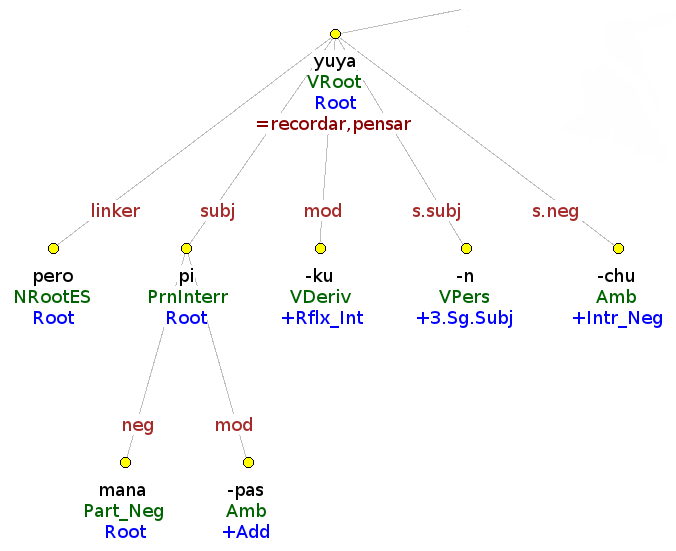
\includegraphics[width=8cm]{tred31.png}}}
\end{center}
\caption{{\em mana} 'narrow scope'}\label{Fig:mananarrow}
\end{figure}
\subparagraph{'dm':}
Cuando 'mana' aparece en una respuesta de una oraci\'on directa, como contrario de {\em ar\'i}, depende de la cabeza de la oraci\'on y recibe la etiqueta 'dm' (marcador de discurso). Considere el ejemplo \ref{Ex:manam}: La primera ocurrencia de {\em mana} se anota con 'dm', la segunda ({\em manam mayistruchu}) en contrario recibe la etiqueta 'neg' (equivale a la diferencia entre p.e. 'no' y 'not' en ingl\'es, o 'nein' y 'nicht' en alem\'an).
\begin{examples}
\item\label{Ex:manam} {\em Mayistruchu? -Manam, manam mayistruchu. Alumnum.} (Ayacuchano)\\
      '{\textquestiondown}Es maestro (\'el)? -No, no es maestro, es alumno.'\\
      	\hfill{\small \citep[17]{Dedenbach02}}
\end{examples}
V\'ease la anotaci\'on en Fig. \ref{Fig:manadm} ('KAN' es un 'dummy element', que se inserta en frases d\'onde la c\'opula (3{\textordfeminine} persona singular) se ha omitido. Ya que anotamos dependencias, necesitamos una cabeza en la frase. Obs\'ervese tambi\'en que el elemento predicativo en oraciones copulativas NO es el verbo auxiliar, sino el sintagma nominal que constituye 'lo que es'. Para m\'as informaci\'on acerca de oraciones con c\'opula, v\'ease tambi\'en p\'arrafo \ref{Sec:copula}. \\
Un ejemplo similar de la anotaci\'on de {\em ar\'i} se encuentra en p\'arrafo \ref{Sec:ari}.

\begin{figure}
\begin{center}\fbox{
\begin{tikzpicture}[scale=0.9]
   \draw (1.5,1) node (text) {\small{\em Manam, manam mayistruchu.}};
    \draw (1.5,0) node (KAN) {KAN};    
  \draw (-2.5,-2) node (mana) {\textcolor{blue}{mana}};
    \draw (-.5,-2) node (m) {-m};
    \draw (2,-2) node (mana2) {mana};      
    \draw (3,-2) node (m2) {-m}; 
    \draw (5.5,-2) node (mayistru) {mayistru}; 
	\draw (5.5,-2.5) node (FOCUS) {\scriptsize{(FOCUS)}}; 
	\draw (5.5,-4) node (-chu) {-chu}; 


     \path[-,color=blue] (mana) edge  node[label=left:\textcolor{blue}{$dm$}]  {} (KAN);
      \path[-] (m) edge  node[label=left:$ev$] {} (KAN);
     \path[-] (mana2) edge  node[label=left:$neg$]{} (KAN);
      \path[-] (m2) edge  node[label=right:$ev$] {} (KAN);
     \path[-] (-chu) edge  node[label=right:$s.neg$] {} (FOCUS);
      \path[-] (mayistru) edge  node[label=above:$pred$] {} (KAN);

\end{tikzpicture}}
 \caption{{\em mana} como marcador de discurso}\label{Fig:manadm}
\end{center}
\end{figure}


  \subsection{{\em ima}}
La part\'icula {\em ima} tiene diferentes usos:
\begin{enumerate}
 \item ra\'iz nominal ('cosa'):\\
       {\em Paqariq warmiyuq wawayuq kanki a lo mejor tocasunki huk warmi mana \textbf{ima}pi yanapakuq.}\\
	'Mañana tendrás mujer e hijos, y a lo mejor te toca una mujer que no te va a ayudar en nada.'\\
	\hfill{\small \citep{Valderrama77}}
 \item posposici\'on coordinativa\\
{\em  ..hinaspataqmi patrón peonta kamachin pagaspa huk uwihirukunaq estancianman saqemunawanpaq hanpiwanankupaq \textbf{ima}.}\\
 '..el patrón ordenó a uno de los peones para que me dejara pagado en una estancia de ovejeros y me curaran de mi mal.'\\
	\hfill{\small \citep{Valderrama77}}
 \item part\'icula interrogativa ('qu\'e?')\\
       {\em \textbf{Ima}n Gregorioyta pasan?}\\
      '{\textquestiondown}Qué le ha pasado a mi Gregorio?\\
	\hfill{\small \citep{Valderrama77}}		
\end{enumerate}

Cada una tiene su anotaci\'on propia. Si {\em ima} se usa como rai\'z nominal con la traducci\'on 'cosa', se anota como cualquier ra\'iz nominal (v\'ease \ref{Sec:nomroot}).\\
Para la anotaci\'on de {\em ima} como posposici\'on coordinativa, v\'ease \ref{Sec:imacoord}.\\
La anotaci\'on de {\em ima} como part\'icula interrogativa es la misma como para una ra\'iz nominal: si lleva un sufijo de caso, \'este constituye la cabeza y depende del verbo seg\'un la funci\'on que tiene (p.e.: {\em imata?} $\rightarrow$ obj, {\em imapaq} $\rightarrow$ ben, etc). Si se usa {\em imataq}, mayormente es el sujeto del verbo y se anota como 'subj'. 


  \subsection{{\em ama}}
En contrario a {\em mana}, la negaci\'on de {\em ama} siempre es 'wide scope', as\'i que {\em ama} siempre depende de la cabeza de la frase como 'neg', v\'ease el ejemplo equivalente de la anotaci\'on de {\em mana} con 'wide scope' en Fig. \ref{Fig:manawide}.


  \subsection{{\em ar\'i}}\label{Sec:ari}
La part\'icula {\em ar\'i} depende de la cabeza de la oraci\'on, y recibe la etiqueta 'dm' (marcador de discurso). V\'ease la anotaci\'on del ejemplo \ref{Ex:ari} en Fig. \ref{Fig:aridm}. 'KAN' es un 'dummy element', que se inserta en frases d\'onde la c\'opula (3{\textordfeminine} persona singular) se ha omitido. Ya que anotamos dependencias, necesitamos una cabeza en la frase. Obs\'ervese tambi\'en que el elemento predicativo en oraciones copulativas NO es el verbo auxiliar, sino el sintagma nominal que constituye 'lo que es'. Para m\'as informaci\'on acerca de oraciones con c\'opula, v\'ease tambi\'en p\'arrafo \ref{Sec:copula}.

\begin{examples}
\item\label{Ex:ari}  {\em Mayistruchu? -Ar\'i, mayistrum.} (Ayacuchano)\\
      '{\textquestiondown}Es maestro? -Si, es maestro.'\\
      	\hfill{\small \citep[16]{Dedenbach02}}
\end{examples}

\begin{figure}
\begin{center}\fbox{
\begin{tikzpicture}[scale=0.9]
   \draw (1.5,1) node (text) {\small{\em Ar\'i, mayistrum.}};
    \draw (1.5,0) node (KAN) {KAN};    
  \draw (-1.5,-2) node (ari) {\textcolor{blue}{ar\'i}};
    \draw (1.5,-2) node (mayistru) {mayistru}; 
    \draw (4.5,-2) node (m) {-m}; 

     \path[-,color=blue] (ari) edge  node[label=left:\textcolor{blue}{$dm$}]  {} (KAN);
      \path[-] (m) edge  node[label=right:$ev$] {} (KAN);
      \path[-] (mayistru) edge  node[label=right:$pred$] {} (KAN);

\end{tikzpicture}}
 \caption{{\em ar\'i}, marcador de discurso}\label{Fig:aridm}
\end{center}
\end{figure}

  \subsection{{\em \~na}}
  La part\'icula {\em \~na} depende del elemento que modifica como 'mod' (modificador). Mayormente depende del verbo, pero no siempre:

\begin{examples}
 \item {\em\textbf{Ña}taq tullu takya -sqa kallpa -yuq -ña ka -nki..}\\
      '-Ahora que ya tienes fuerzas y los huesos duros,..'\\
      $\rightarrow$ depende del verbo, ya que modifica la oraci\'on completa
 \item {\em\textbf{\~Na}n tutataña chayamuyku huk paskana lomadapi kasqa..}\\
      '..ya casi de noche llegamos a una lomadita donde había una posada..'\\
      $\rightarrow$ depende de {\em tuta}, ya que modifica a este elemento ({\em\~Na tutataña} por su parte depende del verbo como 'tmp')
\end{examples}



  \subsection{{\em icha}}
Coordinaciones contrastivas con {\em icha} est\'an descritas en detalle en p\'arrafo \ref{Sec:icha}.
Cuando {\em icha} ({\em ichaqa}) se usa en el sentido de 'pero, en cambio', depende de la cabeza de la oraci\'on (mayormente el verbo finito) como 'linker'.
\begin{examples}
 \item {\em Ichaqa hayapasch\'a kapuliykiqa kashan.}\\
      'Pero tal vez tus capul\'ies son amargos.'
 \item {\em Pipas rikuq kaqtintaqsi ichaqa kaq ratu wa\~nunku.}\\
      'Pero, si algui\'en ha visto, entonces dice que se mueren al instante.'\\
	\hfill{\small \citep[272]{Cusi2}}
\end{examples}
 

\section{Posposiciones}
\subsection{{\em hina,pacha}}\label{Sec:hinaPP}
Las posposiciones {\em hina} y {\em pacha} ('desde') se anotan, igual que los sufijos de caso, como cabeza del sintagma nominal que modifican, mientras que la ra\'iz nominal depende de ellos como 'p.arg' (argumento de posposici\'on). V\'ease tambi\'en p\'arrafo \ref{Sec:hinapachasufijos} para la anotaci\'on de {\em hina} y {\em pacha} como sufijos, y p\'arrafo \ref{Sec:comparacion} para la anotaci\'on de {\em hina} en comparaciones.

\subsubsection{Uso epist\'emico de {\em -chu(s) hina}}\label{Sec:chuhina}

El uso epist\'emico de {\em -chu(s) hina} se anota de la siguiente manera: {\em -chu} depende de {\em hina}, y \'este depende de la cabeza de la oraci\'on (el verbo) como 'epst'. V\'ease la anotaci\'on del ejemplo \ref{Ex:chuhina} en Fig. \ref{Fig:chuhina}.

\begin{examples}
 \item\label{Ex:chuhina} {\em Machuta qhawayukuspa\textbf{chu hina} kayta ruranku.}\\
      Y creo que hacen esto porque a uno le ven viejo.
  \item {\em Pero madrinayqa rikuruwaspa\textbf{chu hina} kusirikun.}\\
      En cambio mi madrina, creo, al verme se alegró [..]\\
      	\hfill{\small \citep{Valderrama77}}
\end{examples}


\begin{figure}
\begin{center}\fbox{
\begin{tikzpicture}[scale=0.9]
   \draw (0,1) node (text) {\small{\em Machuta qhawayukuspa\textbf{chu hina} kayta ruranku.}};
  \draw (2,0) node (rura) {rura};
    \draw (3,-2) node (-ta) {-ta};
      \draw (3,-4) node (kay) {kay};
    \draw (5,-2) node (-nku) {-nku};
    \draw (-3,-2) node (qhawayu) {qhawayu};
      \draw (-6,-4) node (-ta2) {-ta}; 
	\draw (-6,-6) node (Machu) {Machu}; 
      \draw (-3.5,-4) node (-ku) {-ku};
      \draw (-1.5,-4) node (-spa) {-spa};
      \draw (0,-4) node (hina) {\textcolor{blue}{hina}};
      \draw (0,-6) node (-chu) {\textcolor{blue}{-chu}};  
      
     
    

       \path[-,color=blue] (-chu) edge  node[label=right:\textcolor{blue}{$mod$}]  {} (hina);
       \path[-,color=blue] (hina) edge  node[label=right:\textcolor{blue}{$epst$}]  {} (qhawayu);
       \path[-] (-nku) edge  node[label=right:$s.subj$] {} (rura);
       \path[-] (-ta) edge  node[label=left:$obj$] {} (rura);
	    \path[-] (kay) edge  node[label=left:$s.arg$] {} (-ta);
       \path[-] (qhawayu) edge  node[label=above:$sub$] {} (rura);
	         \path[-] (-ta2) edge  node[label=left:$obj$] {} (qhawayu);
	                \path[-] (Machu) edge  node[label=left:$s.arg$] {} (-ta2);
	         \path[-] (-ku) edge  node[label=left:$mod$] {} (qhawayu);
	         \path[-] (-spa) edge  node[label=left:$ns$] {} (qhawayu);

\end{tikzpicture}}
 \caption{Uso epist\'emico de {\em -chu(s) hina}}\label{Fig:chuhina}
\end{center}
\end{figure}

\subsubsection{Uso epist\'emico de {\em hinachu}}\label{Sec:hinachu}

La construcci\'on {\em 'sintagma nominal hinachu'} en el sentido de 'como si fuera, creo que..' se anota de esta forma: {\em hina} es la cabeza del sintagma nominal (label de \'este es 'p.arg'), mientras que {\em -chu} depende del verbo de la oraci\'on como 'epst'. V\'ease la anotacion del ejemplo \ref{Ex:hinachu} en Fig. \ref{Fig:hinachu}.\\
Considere que no cada uso de {\em hinachu} es epist\'emico, v\'ease por ejemplo la anotaci\'on de {\em hinachu icha manachu?} en Fig. \ref{Fig:ichacoord}.


\begin{examples}
 \item\label{Ex:hinachu} {\em Nuqamantaqa yana lunar \textbf{hinachu}, sino mala suerte nuqapi pegasqa.}\\
	    'Yo creo que la mala suerte está en mí pegada como lunar negro.'\\
	        	\hfill{\small \citep{Valderrama77}}
\end{examples}

\begin{figure}
 \begin{center}
\fbox{
\parbox{6cm}{
\centering \vspace{0.5cm}
{\em \small Nuqamantaqa yana lunar hinachu..}\\ \vspace{0.5cm}
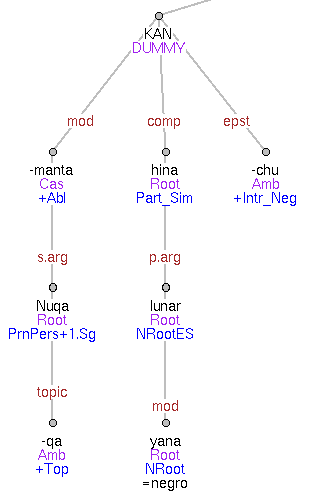
\includegraphics[width=6cm]{tred40.png}
}}
\end{center}
\caption{Anotaci\'on de {\em hinachu} epist\'emico}\label{Fig:hinachu}
\end{figure}


\subsection{Posposici\'on coordinativa {\em ima}}
Coordinaciones con {\em ima} est\'an descritas en p\'arrafo \ref{Sec:imacoord}.

\subsection{Posposiciones locativas}
  \subsubsection{Posesivos}
  PROVISORIO:\\
Las construcciones posesivas con posposiciones se anotan de la misma forma como las construcciones posesivas 'normales'. El 'posesor' recibe la etiqueta 'poss'. La anotaci\'on es diferente de la anotaci\'on de los elementos en yuxtaposici\'on (v\'ease p\'arrafo \ref{Sec:yuxta}).
\begin{examples}
 \item {\em mesa-q pacha -n}\\
	'debajo de la mesa'
  \item {\em wasi -q hawa -n}\\
	'encima de la casa'
 \item {\em inlisa -q laru -n}\\
	'al lado de la iglesia'
 \item {\em qucha -q chawpi -n}\\
       'la parte c\'entrica de la laguna'
 \item {\em wasi -q \~nawpa -n}\\
	'delante de la casa'\\
  		\hfill{\small \citep[140]{Cusi2}}
\end{examples}
V\'ease Fig. \ref{Fig:posposit} para una ilustraci\'on.

\begin{figure}
\begin{center}\fbox{
\begin{tikzpicture}[scale=0.9]
   \draw (-1.5,1) node (text) {\small{\em mesaq pachan}};
   \draw (5,1) node (text) {\small{\em quchaq chawpin}};
    \draw (0,0) node (loc) {}; 
    \draw (-1,-2) node (pacha) {pacha};    
  \draw (1,-3) node (-n) {-n};
    \draw (-3,-3) node (-q) {-q};    
  \draw (-3,-4.5) node (mesa) {mesa};
      \path[-,color=blue] (-q) edge  node[label=left:\textcolor{blue}{$poss$}]  {} (pacha);
       \path[-] (pacha) edge  node[label=left:$loc$] {} (loc);
       \path[-] (-n) edge  node[label=right:$s.poss$] {} (pacha);
       \path[-] (mesa) edge  node[label=left:$s.arg$] {} (-q);


    \draw (7,0) node (loc) {}; 
    \draw (6,-2) node (chawpi) {chawpi};    
  \draw (7,-3) node (-n) {-n};
    \draw (4,-3) node (-q) {-q};    
  \draw (4,-4.5) node (qucha) {qucha};
      \path[-,color=blue] (-q) edge  node[label=left:\textcolor{blue}{$poss$}]  {} (chawpi);
       \path[-] (chawpi) edge  node[label=left:$loc$] {} (loc);
       \path[-] (-n) edge  node[label=right:$s.poss$] {} (chawpi);
       \path[-] (qucha) edge  node[label=left:$s.arg$] {} (-q);

\end{tikzpicture}}
 \caption{Construcciones posesivas con posposiciones}\label{Fig:posposit}
\end{center}
\end{figure}


  \subsubsection{Yuxtaposici\'on}\label{Sec:yuxta}
Posposiciones en yuxtaposici\'on con el elemento que modifican se anotan como cabeza, mientras que la ra\'iz nominal depende de ellos como 'p.arg' (argumento de posposici\'on).

\begin{examples}
 \item {\em wasi pata}\\
      'encima de la casa'
 \item {\em urqu k'uchu}\\
      'al pie del cerro'\\
  		\hfill{\small \citep[140]{Cusi2}}
\end{examples}

V\'ease Fig. \ref{Fig:posyuxta} para una ilustraci\'on.

\begin{figure}
\begin{center}\fbox{
\begin{tikzpicture}[scale=0.9]
    \draw (0,0) node (loc) {}; 
    \draw (-1,-2) node (pata) {pata};       
  \draw (-1,-3.5) node (wasi) {wasi};
      \path[-,color=blue] (wasi) edge  node[label=left:\textcolor{blue}{$p.arg$}]  {} (pata);
       \path[-] (pata) edge  node[label=left:$loc$] {} (loc);

    \draw (7,0) node (loc) {}; 
    \draw (6,-2) node (kuchu) {k'uchu};       
  \draw (6,-3.5) node (urqu) {urqu};
      \path[-,color=blue] (urqu) edge  node[label=left:\textcolor{blue}{$p.arg$}]  {} (kuchu);
       \path[-] (kuchu) edge  node[label=left:$loc$] {} (loc);

\end{tikzpicture}}
 \caption{Yuxtaposici\'on de posposiciones}\label{Fig:posyuxta}
\end{center}
\end{figure}

\section{N\'umeros}
Hay n\'umeros de diferentes tipos, y se distinguen en su anotaci\'on.

  \subsection{N\'umeros complejos}\label{Sec:numcomplejos}
 N\'umeros complejos escritos se anotan de la siguiente manera: La cabeza es el n\'umero m\'as grande (p.e. para n\'umeros de 11-99, la cabeza es {\em chunka}, para n\'umeros de 101-999 es {\em pachak}..), y de ella los dem\'as elementos dependen como 'num'. En caso de las unidades que llevan el sufijo {\em -yuq}: Aqu\'i el n\'umero depende de {\em -yuq} como 's.arg', mientras que {\em -yuq} depende de la cabeza como 'num'. V\'ease Fig. \ref{Fig:2241} como ejemplo.


\begin{figure}
\begin{center}\fbox{
\begin{tikzpicture}
\draw (2.5,1) node (text) {{\em iskay waranqa tawa pachak tawa chunka hukniyuq (2441)}};
  \draw (0,0) node (waranqa) {waranqa};    
  \draw (-2,-2) node (iskay) {iskay};
  \draw (1,-2) node (pachak) {pachak}; 
    \draw (1,-4) node (tawa) {tawa}; 
  \draw (4,-2) node (chunka) {chunka}; 
    \draw (4,-4) node (tawa2) {tawa};
  \draw (7,-2) node (niyuq) {-niyuq}; 
    \draw (7,-4) node (huk) {huk};      

     \path[-] (iskay) edge  node[label=left:{$num$}]  {} (waranqa);
     \path[-] (pachak) edge  node[label=left:{$num$}]  {} (waranqa);
     \path[-] (chunka) edge  node[label=right:{$num$}]  {} (waranqa);
     \path[-] (niyuq) edge  node[label=right:{$num$}]  {} (waranqa);
       \path[-] (tawa) edge  node[label=left:$num$] {} (pachak);
      \path[-] (tawa2) edge  node[label=right:$num$] {} (chunka);
     \path[-] (huk) edge  node[label=right:{$s.arg$}]  {} (niyuq);

\end{tikzpicture}}
 \caption{Anotaci\'on de n\'umeros}\label{Fig:2241}
\end{center}
\end{figure}
  \subsection{Cuantificadores}
  N\'umeros que indican una cantidad de algo se anotan con 'qnt' (quantifier), v\'ease p.e. la anotaci\'on de {\em kinsa alqullantin} en Fig. \ref{Fig:ntin}.\\
  Un caso especial es {\em huk}: No siempre funciona como cuantificador, a veces se usa tambi\'en para acentuar que el sintagma nominal que modifica es indefinido (p.e. {\em huk p'unchay..}), o se usa en el sentido de 'otro'. En estos casos recibe la etiqueta 'mod', no 'qnt'.
Si se trata de n\'umeros complejos escritos, las dependencias internas se anotan como est\'a descrito en p\'arrafo \ref{Sec:numcomplejos}.

\subsection{Modificadores/N\'umeros ordinales}\label{Sec:numord}
N\'umeros que concretizan un sustantivo, no en cantidad, sino m\'as bien como un adjetivo, se anotan como 'mod'. 
\begin{examples}
 \item {5{\textordmasculine} phatmi}\\
	'art\'iculo 5{\textordmasculine}'
 \item\label{Ex:numordKaq} {\em \textbf{Kinsa kaq} pukyu unoqa Arcangelpañataqmi.}\\
	'El agua del tercer manante [sic] es del Arcángel.'\\
		\hfill{\small \citep{Valderrama77}}
 \item {\em iskay chunka \~niqin wasi}\\
      'la vig\'esima casa'
\end{examples}

El elemento {\em \~niqi(n)} depende del n\'umero como 'numord'. En el caso de {\em kaq} se trata de una frase relativa sin cabeza ('el que es tercer'), as\'i que en el ejemplo \ref{Ex:numordKaq} {\em kinsa} es 'pred' de {\em kaq} y este depende de {\em pukyu} como 'mod'.
V\'ease Fig. \ref{Fig:numord} para una ilustraci\'on de los ejemplos.

\begin{figure}
\begin{center}\fbox{
\begin{tikzpicture}[scale=0.9]
    \draw (-1,-2) node (5) {5{\textordmasculine}};    
  \draw (0,0) node (phatmi) {phatmi};
     \path[-,color=blue] (5) edge  node[label=left:\textcolor{blue}{$mod$}]  {} (phatmi);

    \draw (4,0) node (pukyu) {pukyu}; 
    \draw (3,-2) node (ka) {ka}; 
    \draw (2,-4) node (kinsa) {kinsa};   
    \draw (4,-4) node (-q) {-q}; 
      \path[-,color=blue] (ka) edge  node[label=left:\textcolor{blue}{$mod$}] {} (pukyu);
      \path[-] (kinsa) edge  node[label=left:$pred$] {} (ka);
      \path[-] (-q) edge  node[label=right:$ns$] {} (ka);

     \draw (10,0) node (wasi) {wasi};
     \draw (6,-4) node (iskay) {iskay};
     \draw (8,-2) node (chunka) {chunka};
     \draw (10,-4) node (niqin) {\~niqin};

      \path[-,color=blue] (chunka) edge  node[label=left:\textcolor{blue}{$mod$}] {} (wasi);
      \path[-] (iskay) edge  node[label=left:$num$] {} (chunka);
      \path[-] (niqin) edge  node[label=right:$numord$] {} (chunka);

\end{tikzpicture}}
 \caption{N\'umeros ordinales}\label{Fig:numord}
\end{center}
\end{figure}

\subsection{Fechas}

Los n\'umeros en fechas se anotan con 'mod', sean d\'ias, meses o a\~nos, y por convenci\'on (decisi\'on arbitraria), el \'ultimo elemento se anota como cabeza: El d\'ia modifica el mes, el mes modifica el a\~no. La fecha entera por su parte recibe la etiqueta 'tmp' (modificador temporal), v\'ease Fig. \ref{Fig:fecha}.

\begin{figure}
\begin{center}\fbox{
\begin{tikzpicture}[scale=0.9]
   \draw (2,1) node (text) {\small{\em 29 p'unchaw septiembre killapi 2005 watapi}};
    \draw (0,0) node (tmp) {};    
  \draw (2,-1) node (-pi) {-pi}; 
    \draw (2,-3) node (wata) {wata}; 
    \draw (1,-5) node (2005) {2005}; 
    \draw (3,-5) node (-pi2) {-pi};    
     \draw (3,-7) node (killa) {killa};
     \draw (1,-8.5) node (septiembre) {septiembre};
     \draw (5,-8.5) node (punchaw) {p'unchaw};
     \draw (5,-9.8) node (29) {29};

       \path[-,color=blue] (-pi) edge  node[label=above:\textcolor{blue}{$tmp$}] {} (tmp);
      \path[-] (wata) edge  node[label=left:$s.arg$] {} (-pi);
       \path[-] (2005) edge  node[label=left:$mod$] {} (wata);
       \path[-] (-pi2) edge  node[label=right:$mod$] {} (wata);
       \path[-] (killa) edge  node[label=right:$s.arg$] {} (-pi2);
       \path[-] (septiembre) edge  node[label=left:$mod$] {} (killa);
       \path[-] (punchaw) edge  node[label=right:$mod$] {} (killa);
       \path[-] (29) edge  node[label=right:$mod$] {} (punchaw);

\end{tikzpicture}}
 \caption{Anotaci\'on de fecha}\label{Fig:fecha}
\end{center}
\end{figure}


\subsection{Indicaci\'on de la hora}
Los n\'umeros espa\~noles que indican una hora del d\'ia, y llevan uno de los sufijos de caso {\em -ta} o {\em -paq}, son argumentos de \'estos y reciben la etiqueta 's.arg'. El art\'iculo espa\~nol depende del n\'umero como 'mod'. La hora entera por su parte se anota como modificador temporal ('tmp').
\begin{examples}
 \item {\em Las uchutam yaykuni iskwilaman.}\\
      'A las ocho entro a la escuela.'
 \item\label{Ex:dusi} {\em Las dusipaqqa puka pikanti kanqa.}\\
      'A las doce habr\'a puka pikanti.'\\
  		\hfill{\small \citep[70]{Dedenbach02}}
\end{examples}

V\'ease Fig. \ref{Fig:hora} para una ilustraci\'on del ejemplo \ref{Ex:dusi}.

\begin{figure}
\begin{center}\fbox{
\begin{tikzpicture}[scale=0.9]
   \draw (0,1) node (text) {\small{\em Las dusipaqqa puka pikanti kanqa.}};
  \draw (0,0) node (kanqa) {kanqa};
    \draw (-3,-1) node (-paq) {-paq}; 
    \draw (-2,-5) node (-qa) {-qa}; 
    \draw (-3,-3) node (dusi) {dusi};    
     \draw (-4,-5) node (las) {las};
     \draw (3,-1) node (pikanti) {pikanti};
     \draw (3,-3) node (puka) {puka};

      \path[-,color=blue] (-paq) edge  node[label=above:\textcolor{blue}{$tmp$}] {} (kanqa);
      \path[-] (dusi) edge  node[label=left:$s.arg$] {} (-paq);
      \path[-] (las) edge  node[label=left:$mod$] {} (dusi);
      \path[-] (-qa) edge  node[label=right:$topic$] {} (dusi);
      \path[-] (pikanti) edge  node[label=above:$subj$] {} (kanqa);
      \path[-] (puka) edge  node[label=right:$mod$] {} (pikanti);
\end{tikzpicture}}
 \caption{Indicaci\'on de hora con n\'umeros espa\~noles}\label{Fig:hora}
\end{center}
\end{figure}

\section{Interjecciones}
Interjecciones de todo tipo se anotan con 'dm' (marcador de discurso). Interjecciones son p.e. {\em achach\'aw, alal\'aw, akhak\'aw, a\~na\~n\'aw} etc., peor tambi\'en {\em yaw, an, chuy, ah\'ay, ma} etc.

\section{Abreviaciones}

Abreviaciones se anotan seg\'un la funci\'on que tienen en la oraci\'on. Si la frase abreviado aparece junto a la abreviaci\'on en par\'entesis, la abreviaci\'on depende de la frase como 'abbrev'. V\'ease tambi\'en Fig. \ref{Fig:abbrev} para un ejemplo (las etiquetas en las relaciones internas de la frase espa\~nola quedan sin especificar ($--$)).

\begin{examples}
 \item {\em ..Documentos de Estrategias de Reducción de la Pobreza (PRSP) sutichasqa}
  \item {\em ..dióxido de carbono (CO2) nisqa}
\end{examples}

\begin{figure}
\begin{center}\fbox{
\begin{tikzpicture}[scale=0.9]
   \draw (-1,1) node (text) {\small{\em ..dióxido de carbono (CO2) nisqa}};
    \draw (0,0) node (ni) {ni};    
     \draw (1,-2) node (-sqa) {-sqa};
  \draw (-2,-2) node (dio) {di\'oxido};
    \draw (-2,-4) node (de) {de}; 
    \draw (-2,-6) node (carbono) {carbono}; 
    \draw (-1,-4) node (CO2) {CO2}; 

      \path[-,color=blue] (CO2) edge  node[label=right:\textcolor{blue}{$abbrev$}] {} (dio);
      \path[-] (dio) edge  node[label=left:$flm$] {} (ni);
       \path[-] (de) edge  node[label=left:\tiny{$--$}] {} (dio);
       \path[-] (carbono) edge  node[label=left:\tiny{$--$}] {} (de);
       \path[-] (-sqa) edge  node[label=right:$ns$] {} (ni);
\end{tikzpicture}}
 \caption{Abreviaciones}\label{Fig:abbrev}
\end{center}
\end{figure}

\section{Nombres}

Nombres complejos que contienen varias palabras se anotan de la siguiente manera: El apellido es la cabeza, si hay m\'as que un apellido, el primero es la cabeza. Todos los dem\'as partes del nombre, sean t\'itulos o nombres, dependen de \'el como 'nme' ('name'). V\'ease la anotaci\'on de 'Gregorio Mamani' en Fig. \ref{Fig:KAN} o de 'Tupaq Amaru' en Fig. \ref{Fig:jusivo}.


\section{Oraciones}\label{Sec:oraciones}
\subsection{Coordinaci\'on}\label{Sec:coord}

\subsubsection{Coordinaciones con 'doble' sufijo}\label{Sec:coorddoble}
Coordinaci\'ones del tipo '[elemento coordinado 1] --[sufijo coordinativo] [elemento coordinado 2] --[sufijo coordinativo]'  se anotan de esta manera: el sufijo coordinativo depende del elemento coordinado como 's.co', y el primer elemento coordinado depende como 'co' del \'ultimo elemento, v\'ease Fig. \ref{Fig:Coord}. 


\begin{figure}
\begin{center}\fbox{
\begin{tikzpicture}
    \draw (1,-1.5) node (palabra1) {palabra1};
      \draw (1,-3) node (sufijo1) {sufijo coordinativo};
   \draw (6,0) node (palabra2) {palabra2};
      \draw (6,-1.5) node (sufijo2) {sufijo coordinativo};

     \path[-] (sufijo1) edge  node[label=left:$s.co$] {} (palabra1);
     \path[-] (sufijo2) edge  node[label=left:$s.co$] {} (palabra2);
     \path[-] (palabra2) edge  node[label=left:$co$] {} (palabra1);

\end{tikzpicture}}
\caption{Esquema de coordnaci\'on 'doble-marcada'}\label{Fig:Coord}
\end{center}
\end{figure}

Coordinaciones de este tipo ocurren con los siguientes sufijos:

\begin{itemize}
 \item {\em -pas/-pis}:\\
      {\em Paqay\textbf{pis} paltay\textbf{pis} kanmi yunkapi.}\\
      'En el valle, adem\'as hay pacae y palta.
 \item {\em -taq}:\\
      {\em Mangoqa chhapu ruru\textbf{taq} hillisapa\textbf{taq} hinan.}\\
      'El mango se caracteriza tanto por tener una pepa fibrosa como por tener bastante jugo.'\\
	\hfill{\small \citep[141-143]{Cusi2}}
 \item {\em -chu} en combinaci\'on con {\em icha} o una part\'icula espa\~nola (ni, o(taq), etc)\\
       v\'ease \ref{Sec:icha}
\end{itemize}

Coordinaciones con dos sufijos de caso como en el ejemplo \ref{Ex:coordwan} se anotan de la siguiente manera:
Los sufijos de caso son las cabezas de 'sus' palabras, y el \'ultimo es la cabeza de la coordinaci\'on, v\'ease Fig. \ref{Fig:coordwan} para una ilustraci\'on esquem\'atica o v\'ease tambi\'en \ref{Fig:wanco} para un ejemplo con el sufijo {\em -wan}.

\begin{examples}
 \item\label{Ex:coordwan} {\em -wan/-puwan}:\\
      {\em Taytay\textbf{wan} mamay\textbf{puwan}mi llaqtataqa rinku.}\\
      'Al pueblo fueron mi pap\'a y mi mam\'a.'
	\hfill{\small \citep[141-143]{Cusi2}}
\end{examples}


\begin{figure}
\begin{center}\fbox{
\begin{tikzpicture}
    \draw (1,-3) node (palabra1) {palabra1};
      \draw (1,-1.5) node (sufijo1) {sufijo de caso};
   \draw (6,-1.5) node (palabra2) {palabra2};
      \draw (6,0) node (sufijo2) {sufijo de caso};

     \path[-] (sufijo1) edge  node[label=left:$s.arg$] {} (palabra1);
     \path[-] (sufijo2) edge  node[label=left:$s.arg$] {} (palabra2);
     \path[-] (sufijo1) edge  node[label=left:$co$] {} (sufijo2);

\end{tikzpicture}}
\caption{Esquema de coordnaci\'on 'doble-marcada' con sufijos de caso}\label{Fig:coordwan}
\end{center}
\end{figure}

Un caso especial son las coordinaciones con sufijos coordinativos que comparten un modificador (que modifica la coordinci\'on entera). V\'ease p\'arrafo \ref{Sec:coordmod} y especialmente Fig. \ref{Fig:comodSuffix} para la anotaci\'on de estas construcciones.

  \subsubsection{{\em ima}}\label{Sec:imacoord}
  Si {\em ima} se usa como posposici\'on coordinativa, los elementos coordinados dependen del \'ultimo elemento coordinado, mientras que  {\em ima} depende de este como 'linker'.
\begin{examples}
 \item {\em  ..hinaspataqmi patrón peonta kamachin pagaspa huk uwihirukunaq estancianman saqimunawanpaq hanpiwanankupaq \textbf{ima}.}\\
 '..el patrón ordenó a uno de los peones para que me dejara pagado en una estancia de ovejeros y me curaran de mi mal.'\\
    v\'ease Fig. \ref{Fig:imacoord} para una ilustraci\'on simplificada.\\
	\hfill{\small \citep{Valderrama77}}
\end{examples}

\begin{figure}
\begin{center}\fbox{
  \begin{tikzpicture}
   \draw (-2,-2) node (saqimunawanpaq) {saqimunawanpaq};
   \draw (2,-2) node (ima) {ima};
   \draw (0,-0) node (hanpiwanankupaq) {hanpiwanankupaq};

     \path[-] (ima) edge  node[label=right:$linker$] {} (hanpiwanankupaq);
     \path[-] (saqimunawanpaq) edge  node[label=left:$co$] {} (hanpiwanankupaq);

\end{tikzpicture}}
\caption{{\em ima} como posposici\'on coordinativa (simplificado)}\label{Fig:imacoord}
\end{center}
\end{figure}

\subsubsection{{\em icha}}\label{Sec:icha}
La part\'icula contrastiva {\em icha} ('o') depende del segundo elemento coordinativo como 'linker', y el primer elemento de la coordinaci\'on depende del segundo como 'co'. V\'ease la anotaci\'on de la frase  {\em Hinachu \textbf{icha} manachu?} ('{\textquestiondown}Es as\'i o no?') en Fig. \ref{Fig:ichacoord}.

\begin{figure}
\begin{center}\fbox{
 \begin{tikzpicture}
   \draw (4,1) node (text) {\small{\em Hinachu icha manachu?}};
     \draw (1,-1.5) node (Hina) {Hina};
      \draw (1,-3) node (-chu) {-chu};
   \draw (6,-0) node (mana) {mana};
      \draw (4,-2) node (icha) {icha};
      \draw (8,-1.5) node (-chu2) {-chu};

     \path[-] (-chu) edge  node[label=right:$s.co$] {} (Hina);
     \path[-] (-chu2) edge  node[label=right:$s.co$] {} (mana);
     \path[-] (icha) edge  node[label=left:$linker$] {} (mana);
     \path[-] (mana) edge  node[label=above:$co$] {} (Hina);
\end{tikzpicture}}
\caption{Coordinaci\'on contrastiva con {\em icha}}\label{Fig:ichacoord}
\end{center}
\end{figure}


\subsubsection{Part\'iculas espa\~nolas}
Las part\'iculas coordinativas tomadas del espa\~nol se anotan de la misma forma como {\em icha}. Son las siguientes: {\em o (u,otaq), ni, y}.

\begin{examples}
 \item {\em Munaspaqa mut'itapas \textbf{otaq} phusputapas huqarikuy.}\\
	'Si gustas puedes servirte el mote o las habas sancochadas.'
 \item {\em Manan uywaypas \textbf{ni} chakraypas kanchu.}\\
      'No tengo tampoco ni animales ni tierra.'\\
	v\'ease Fig. \ref{Fig:nicoord}\\
	\hfill{\small \citep[142-143]{Cusi2}}
\end{examples}

\begin{figure}
\begin{center}\fbox{
 \begin{tikzpicture}
   \draw (4,1) node (text) {\small{\em uywaypas ni chakraypas}};
     \draw (1,-1.5) node (uyway) {uyway};
      \draw (1,-3) node (-pas) {-pas};
   \draw (6,0) node (chakray) {chakray};
      \draw (4,-2) node (ni) {ni};
      \draw (8,-1.5) node (-pas2) {-pas};

     \path[-] (-pas) edge  node[label=left:$s.co$] {} (uyway);
     \path[-] (-pas2) edge  node[label=right:$s.co$] {} (chakray);
     \path[-] (ni) edge  node[label=left:$linker$] {} (chakray);
     \path[-] (chakray) edge  node[label=above:$co$] {} (uyway);
\end{tikzpicture}}
\caption{Coordinaci\'on con {\em ni} (simplificado)}\label{Fig:nicoord}
\end{center}
\end{figure}



\subsubsection{Coordinaci\'on de dos oraciones finitas}
CAMBIADO:\\
Coordinaciones de dos (o m\'as) oraciones con verbos finitos se anotan de la forma siguente: Si son dos oraciones en yuxtaposici\'on, \'ultima es la cabeza, la primera depende de \'esta como 'co'. Cuando son m\'as que dos oraciones coordinadas en yuxtaposici\'on, la \'ultima es la cabeza de la que todas las dem\'as dependen. \\
Si una de las oraciones tiene un elemento coordinativo como {\em otaq, chaytaq} etc., \'este depende de la cabeza de 'su' oraci\'on como 'linker'.  V\'ease la anotaci\'on esquem\'atica en Fig. \ref{Fig:linkercoord}.\\
Oraciones con part\'iculas como \textit{chaymi, chaymantataq, sichus} etc. no son coordinadas sino sbuordinadas, v\'ease p\'arrafo \ref{Sec:SubFinita}.\\


\begin{examples}
  \item {\em Phaway tiyuykiq wasinta rirqunki, \textbf{hinaspa} asnonta ma\~narakamunki.}\\
      'Anda, corre, a la casa de tu t\'io, y entonces te prestas sus burros.'\\
  	\hfill{\small \citep[272]{Cusi2}}
\end{examples}

\begin{figure}
\begin{center}\fbox{
 \begin{tikzpicture}
   \draw (1,1) node (text) {\small{en yuxtaposici\'on:}};
     \draw (-1,-2) node (oracion1) {oracion1};
   \draw (2,0) node (oracion2) {oracion2};

   \draw (7,1) node (text2) {\small{con linker:}};
     \draw (6,-2) node (oracion3) {oracion1};
   \draw (9,0) node (oracion4) {oracion2};
      \draw (9,-2) node (linker) {$otaq/etc$};

     \path[-] (linker) edge  node[label=right:$linker$] {} (oracion4);
     \path[-] (oracion2) edge  node[label=left:$co$] {} (oracion1);
     \path[-] (oracion3) edge  node[label=left:$co$] {} (oracion4);

\end{tikzpicture}}
\caption{Esquema coordinaci\'on de dos oraciones finitas}\label{Fig:linkercoord}
\end{center}
\end{figure}

\subsubsection{Yuxtaposici\'on coordinativa}\label{Sec:coordyuxta}

En coordinaciones de dos sustantivos en yuxtaposici\'on, el primer elemento depende del segundo como 'co'.

\begin{examples}
 \item {\em tayta mama}\\
      'padres de familia'
  \item {\em tuta p'unchaw}\\
      'd\'ia y noche'
\item {\em wichay uray}\\
      'arriba y abajo'\\
	\hfill{\small \citep[133]{Cusi2}}
\end{examples}

\subsubsection{Modificadores de Coordinaciones}\label{Sec:coordmod}

Elementos dependientes de la cabeza de una coordinaci\'on son ambiguos en el sentido de que no queda claro si modifican s\'olo a la cabeza o la coordinac\'on entera si en los dos casos se usa la misma etiqueta. Para resolver esta ambig\"uedad en la anotaci\'on, usamos dos etiquetas distintas: 'co:+funci\'on' (p.e. 'co:mod') si el elemento modifica la coordinaci\'on entera, y la etiqueta simple si modifica s\'olo la cabeza.\\
Considera los ejemplos \ref{Ex:coloc} y \ref{Ex:locco}: En ambos casos, en modificador locativo {\em kaypi} depende de la cabeza de la coordinaci\'on {\em pukllanku}, pero en \ref{Ex:coloc} modifica la coordinaci\'on entera, y por eso recibe la etiqueta 'co:loc'. En ejemplo \ref{Ex:locco}, en cambio, modifica s\'olo {\em pukllanku}, no la coordinaci\'on entera, por eso recibe la simple etiqueta 'loc'.
\begin{center}
 \begin{minipage}{0.4\textwidth}
 \begin{examples}
 \item\label{Ex:coloc} {\em kaypi llank'anku, punkllanku ima}\\
      trabajan y juegan aqu\'i
  \item\label{Ex:locco} {\em (chaypi) llank'anku,  kaypi punkllanku}\\
      trabajan (all\'a) y juegan aqu\'i
\end{examples}
\end{minipage}
\hfill
\begin{minipage}{0.5\textwidth}
\begin{center}\fbox{
\begin{tikzpicture}
      \draw (-4,0.5) node (1) {ejemplo \ref{Ex:coloc}:};
      \draw (0,0) node (pukllanku) {pukllanku};
  \draw (-1,-2) node (llank'anku) {llank'anku};
      \draw (1,-1) node (ima) {ima};
  \draw (-4,-2) node (kaypi) {\textcolor{blue}{kaypi}};
      \path[-] (llank'anku) edge  node[label=left:$co$]{} (pukllanku);
      \path[-,color=blue] (kaypi) edge  node[label=left:\textcolor{blue}{$co:loc$}]  {} (pukllanku);
      \path[-] (ima) edge  node[label=right:$linker$]  {} (pukllanku);
%%%%%%%%%%%%%%%%%%%%%%%%%%%%%%%%%%%%%%%%%%%%%%%%%%%%%%%%%%%%%%%%%%%%%%%
       \draw (-4,-3) node (2) {ejemplo \ref{Ex:locco}:};    
      \draw (0,-3.5) node (pukllanku2) {pukllanku};
  \draw (-3,-5.5) node (llank'anku2) {llank'anku};
  \draw (0,-5.5) node (kaypi2) {\textcolor{blue}{kaypi}};
      \path[-] (llank'anku2) edge  node[label=left:$co$]{} (pukllanku2);
      \path[-,color=blue] (kaypi2) edge  node[label=left:\textcolor{blue}{$loc$}]  {} (pukllanku2);

\end{tikzpicture}}
% \caption{Ra\'iZ nominal compuesta}\label{Fig:NRootCMP}
\end{center}
\end{minipage}
\end{center}

En caso de una coordinaci\'on con sufijos coordinativos (v\'ease \ref{Sec:coorddoble}), un modificador que modifica a la coordinaci\'on entera no depende del sufijo coordinativo que es la cabeza de la coordinaci\'on, sino de la ra\'iz que pertenece a este sufijo, ya que no modifica a los sufijos coordinativos sino a las ra\'ices. V\'ease el ejemplo \ref{Ex:comodSuffix} :\\
La cuantificaci\'on {\em pachaq pachaq} modifica a la coordinaci\'on entera, por eso depende como 'co:qnt' de la \'ultima ra\'iz coordinada. V\'ease Fig. \ref{Fig:comodSuffix} para la anotaci\'on.

\begin{examples}
 \item\label{Ex:comodSuffix} {\em Kunanqa manan ñawpaq hinañachu, gentepas Puno qucha wichay ladomantaraq \textbf{pachaq pachaq llamakunapi caballokunapi asnokunapi} hamuq.}\\
	Ahora ya no es como antes, donde la gente venía desde el lago de Puno, en cientos y cientos de llamas, caballos, asnos.\\
	  	\hfill{\small \citep{Valderrama77}}
\end{examples}

\begin{figure}

 \begin{center}
\fbox{
\parbox{12cm}{
\centering \vspace{0.5cm}
{\em \small ..Puno qucha wichay ladomantaraq pachaq pachaq llamakunapi caballokunapi asnokunapi hamuq.}\\ \vspace{0.5cm}
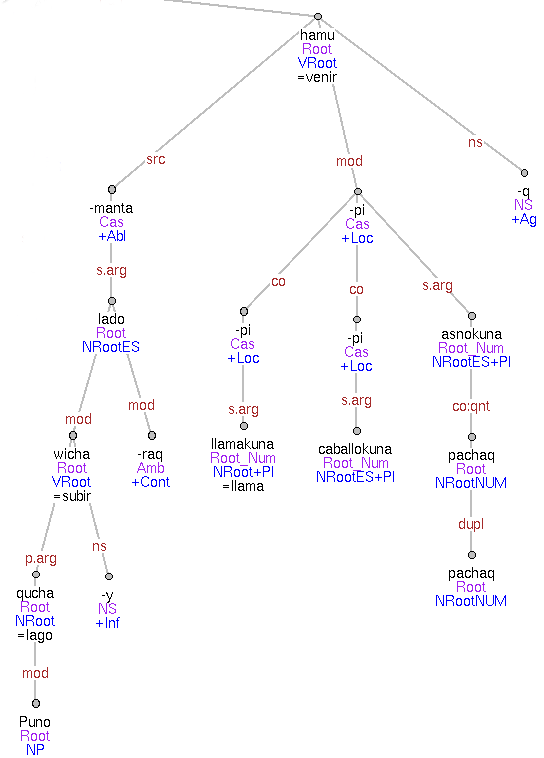
\includegraphics[width=12cm]{tred41.png}
}}
\end{center}
\caption{Coordinaci\'on con sufijos coordinativos y modificador}\label{Fig:comodSuffix}
\end{figure}



% \begin{center}
%  \begin{minipage}{0.4\textwidth}
%  \begin{examples}
%  \item {\em chhayna hatun thanta wasi}\\
%      1. 'casa [tan [grande y vieja]]'\\
%      2. 'casa [tan grande] y vieja]
% \end{examples}
% \end{minipage}
% \hfill
% \begin{minipage}{0.5\textwidth}
% \begin{center}\fbox{
% \begin{tikzpicture}
%       \draw (-4,0.5) node (1) {1. interpretaci\'on:};
%       \draw (0,0) node (wasi) {wasi};
%   \draw (-1,-1) node (thanta) {thanta};
%       \draw (-1,-2) node (hatun) {hatun};
%   \draw (-4,-2) node (chhayna) {\textcolor{blue}{chhayna}};
%       \path[-] (hatun) edge  node[label=left:$co$]{} (thanta);
%       \path[-,color=blue] (chhayna) edge  node[label=left:\textcolor{blue}{$co:mod$}]  {} (thanta);
%       \path[-] (thanta) edge  node[label=left:$mod$]  {} (wasi);
% %%%%%%%%%%%%%%%%%%%%%%%%%%%%%%%%%%%%%%%%%%%%%%%%%%%%%%%%%%%%%%%%%%%%%%%
%       \draw (-4,-3) node (2) {2. interpretaci\'on:};    
%       \draw (0,-3.5) node (wasi) {wasi};
%   \draw (-0.5,-4.5) node (thanta) {thanta};
%       \draw (-1,-5.5) node (hatun) {hatun};
%   \draw (-1.5,-6.5) node (chhayna) {\textcolor{blue}{chhayna}};
%       \path[-] (hatun) edge  node[label=left:$co$]{} (thanta);
%       \path[-,color=blue] (chhayna) edge  node[label=left:\textcolor{blue}{$mod$}]  {} (hatun);
%       \path[-] (thanta) edge  node[label=left:$mod$]  {} (wasi);
% 
% \end{tikzpicture}}
% % \caption{Ra\'iZ nominal compuesta}\label{Fig:NRootCMP}
% \end{center}
% %\end{figure}
% \end{minipage}
% \end{center}

\subsubsection{Elisi\'on de verbo finito en coordinaciones}
Con coordinaciones a nivel de oraciones que comparten el mismo verbo, es posible que el verbo de una de las oraciones se elide.\\
IMPORTANTE: si las dos oraciones NO comparten todos los modificadores a nivel de oraci\'on (sujeto, linker, negaci\'on, evidencialidad), es necesario asumir dos oraciones coordinadas. V\'ease los ejemplos \ref{Ex:elision1} y \ref{Ex:elision2}:

\begin{examples}
 \item\label{Ex:elision1} {\em Khayna Pachamama (kan) kay p'unchaykunalla muhuta munan, \textcolor{MidnightBlue}{mana qollori p'unchaykunachu.}}\\
	Así es la pachamama que quiere la semilla sólo estos días y no los otros que son qollori.\\
	 	\hfill{\small \citep{Valderrama77}}
\item\label{Ex:elision2} {\em Iskay laymi kaq (kan), sapanka laymipitaq papa tarpukuq (kan) askha ladopi \textcolor{MidnightBlue}{mana hukllapichu.}}\\
      Había dos laymes y en cada layme la papa se sembraba en varios lugares y nunca en un solo sitio.\\
	 	\hfill{\small \citep{Valderrama77}}
\end{examples}

En {\em mana qollori p'unchaykunachu} de la frase \ref{Ex:elision1} falta el verbo {\em munan}. Nota que en este caso no es posible anotar la coordinaci\'on a nivel del sintagma nominal, porque la negaci\'on {\em mana} debe depender del verbo. En este caso es necesario insertar un elemento artificial ('dummy') que es la ra\'iz verbal que falta ('muna'). Los elementos de la primera oraci\'on que faltan en la segunda ahora se a\~naden como 'secondary edges': se a\~nade un atributo  'secedges' en dicho nodo, y entonces hay que insertar el valor de 'id' del dummy en 'idref' (el punto terminal de la flecha que se va a a\~nadir). Tambi\'en hay que insertar la etiqueta de la relaci\'on en 'secedgelabel', normalmente ser\'a la misma como en 'label'.\\
As\'i que en el ejemplo \ref{Ex:elision1}, se inserta un dummy 'MUNA' y se a\~nade un 'secedge' desde el nodo {\em -n} de la primera oraci\'on, con la etiqueta 's.subj'. V\'ease la anotaci\'on en Fig. \ref{Fig:elision1}.\\
En el ejemplo \ref{Ex:elision2}, el verbo elidido de la segunda oraci\'on es {\em tarpu}, y ya que es la forma del pasado habitual de tercera persona, tambi\'en hay que insertar un 'dummy' para la copula (TARPU y KAN), v\'ease la anotaci\'on en Fig. \ref{Fig:elision2}.

\begin{figure}
 \begin{center}
\fbox{
\parbox{\textwidth}{
\centering \vspace{0.5cm}
{\em \small Khayna Pachamama (kan) kay p'unchaykunalla muhuta munan, \textcolor{MidnightBlue}{mana qollori p'unchaykunachu.}}\\ \vspace{0.5cm}
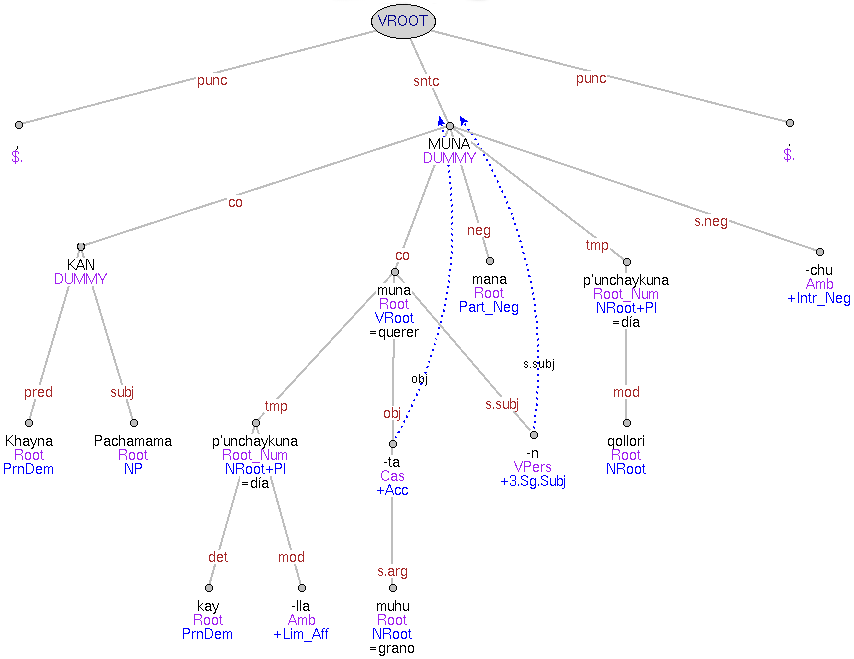
\includegraphics[width=\textwidth]{tred49.png}
}}
\end{center}
\caption{Elisi\'on de verbo finito en coordinaci\'on}\label{Fig:elision1}
\end{figure}

\begin{figure}
 \begin{center}
\fbox{
\parbox{\textwidth}{
\centering \vspace{0.5cm}
{\em \small Iskay laymi kaq (kan), sapanka laymipitaq papa tarpukuq (kan) askha ladopi \textcolor{MidnightBlue}{mana hukllapichu.}}\\ \vspace{0.5cm}
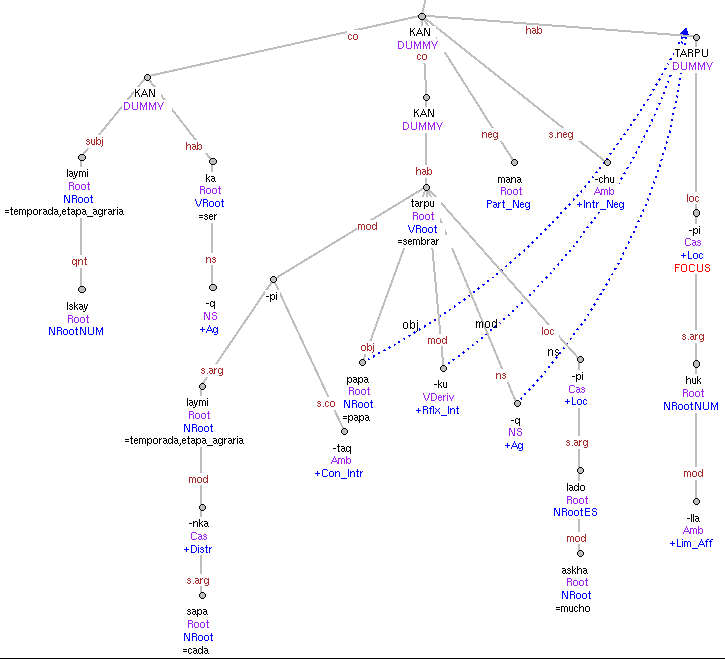
\includegraphics[width=\textwidth]{tred50.png}
}}
\end{center}
\caption{Elisi\'on de verbo finito en coordinaci\'on, pasado habitual 3$^a$ persona}\label{Fig:elision2}
\end{figure}

\subsection{Subordinaci\'on}

\subsubsection{Formas no-finitas}

\paragraph{Switch reference}

Frases que contienen una forma nominalizado del verbo por uno de los sufijos {\em  -qti, -stin, -spa} dependen de la oraci\'on principal como 'sub'. V\'ease la anotaci\'on del ejemplo \ref{Ex:linkerswitch} en Fig. \ref{Fig:linkerswitch}.

\begin{examples}
 \item {\em Allinta qhawarispa purinki.}\\
	'Has de caminar mirando bien.'
 \item {\em Atispaykiqa ruwayy\'a!}\\
	'{\textexclamdown}Si puedes, hazlo, pues!'
 \item {\em Tarpustillan\~na ruwamusunman chaych\'a allinqa kanman.}\\
      '{\textexclamdown}Qu\'e bueno ser\'ia si labramos y luego realizamos la siembra!'
 \item\label{Ex:linkerswitch} {\em Pay hamuqtin\~na kamachinakusunchis.}\\
      'Ya nos pondremos de acuerdo cu\'ando \'el viene.'
 	\hfill{\small \citep[209-214]{Cusi2}}
\end{examples}

\begin{figure}
\begin{center}\fbox{
 \begin{tikzpicture}
   \draw (-2,1) node (text) {\small{\em Pay hamuqtin\~na kamachinakusunchis.}};
     \draw (0,0) node (kamachinaku) {kamachinaku};
   \draw (1,-2) node (-sunchis) {-sunchis};
      \draw (-3,-2) node (hamu) {hamu};
      \draw (-5,-4) node (Pay) {Pay};
      \draw (-3,-4) node (-qti) {-qti};
      \draw (-1,-4) node (-nia) {\~na};

     \path[-] (-nia) edge  node[label=right:$mod$] {} (hamu);
     \path[-] (-qti) edge  node[label=left:$ns$] {} (hamu);
     \path[-] (Pay) edge  node[label=left:$subj$] {} (hamu);
     \path[-,color=blue] (hamu) edge  node[label=left:\textcolor{blue}{$sub$}] {} (kamachinaku);
     \path[-] (-sunchis) edge  node[label=right:$s.subj$] {} (kamachinaku);

\end{tikzpicture}}
\caption{Switch reference}\label{Fig:linkerswitch}
\end{center}
\end{figure}


\paragraph{Formas nominales}\label{Sec:subordNom}
Nominalizaciones con los sufijos {\em -sqa, -na} o {\em -y} (infinitivo), dependen de la oraci\'on principal seg\'un el sufijo de caso que llevan. La frase nominal entonces depende del sufijo de caso como 's.arg.claus', NO como 's.arg'. \\
Si la forma nominalizada lleva un sufijo acusativo y es un argumento del verbo, recibe la etiqueta 'obj',
v\'ease p.e. Fig. \ref{Fig:taclause} para un ejemplo con el infinitivo, o Fig. \ref{Fig:manawide} para un ejemplo con {\em -na}.\\
Con el sufijo de caso {\em -paq} ('para que') recibe la etiqueta 'purp' ('purposive'), v\'ease tambien p\'arrafo \ref{Sec:paqpurp} o la figura \ref{Fig:paqpurp}.\\
La combinaci\'on {\em -na} y {\em -kama} ('hasta que') se anota como 'sub', v\'ease p\'arrafo \ref{Sec:kamasub}.\\
La combinaci\'on {\em -sqa} y {\em -pi} ('mientras') se anota como 'sub', v\'ease p\'arrafo \ref{Sec:pisub}.\\
La combinaci\'on de {\em na} y {\em -rayku} resulta en una frase final y tambi\'en recibe la etiqueta 'purp', v\'ease p\'arrafo \ref{Sec:raykupurp}.\\
La combinaci\'on {\em -sqa} y {\em -rayku} ('por/porque') se anota con 'caus'.\\
La construcci\'on {\em -na} m\'as una forma finita de la copula se anota con 'oblg' (obligaci\'on), v\'ease p\'arrafo \ref{Sec:nakay}.

\begin{examples}
 \item {\em Ventanata kichay wayraq haykurimunanpaq.}\\
      'Abre la ventana para que entre el aire.'
 \item {\em Kayllapi suyawashanki kutiramunaykama.}\\
      'Vas a estar esper\'andome aqu\'i no m\'as hasta que regrese.'
 \item {\em Aman chay yachasqaykita qunqankichu.}\\
      'No vas a olvidarte eso que has aprendido.'
 \item {\em Munankichu llank'akuyta?}\\
      '{\textquestiondown}Quieres trabajar?'\\
 	\hfill{\small \citep[209-214]{Cusi2}}
\end{examples}



\paragraph{Oraciones relativas}\label{Sec:relclause}
Los nominalizadores {\em -na, -sqa} y {\em -q} tambi\'en pueden formar oraciones relativas, en este caso reciben la etiqueta 'mod' y dependen del sustantivo que modifican.

\begin{examples}
 \item {\em Pitaq chahay machasqa runari?}\\
      '{\textquestiondown}Y qui\'en ser\'a aquel hombre borracho?\\
 	\hfill{\small \citep[209-214]{Cusi2}}
 \item\label{Ex:relclause} {\em Wasi ruwaq runa hamuchkan.} (Ayacuchano)\\
      'Viene el hombre que hace casas.'
 \item {\em Apamusqan wallpa wacharun\~na.} (Ayacuchano)\\
      'La gallina que trajo ya puso huevos.'
\item {\em Wayqa sirana yawrita apamuy.} (Ayacuchano) \\
      'Trae la aguja de coser talegos.'\\
 	\hfill{\small \citep[153]{Soto76a}}
\end{examples}

V\'ease Fig. \ref{Fig:relclause} para una ilustraci\'on del ejemplo \ref{Ex:relclause}.

\begin{figure}
\begin{center}\fbox{
 \begin{tikzpicture}
   \draw (-1,1) node (text) {\small{\em Wasi ruwaq runa hamuchkan.}};
     \draw (0,0) node (hamu) {hamu};
   \draw (1,-2) node (-chkan) {-chkan};
      \draw (-1,-2) node (runa) {runa};
      \draw (-2,-4) node (ruwa) {ruwa};
      \draw (-3,-6) node (wasi) {wasi};
      \draw (-1,-6) node (-q) {-q};

      \path[-] (wasi) edge  node[label=left:$obj$] {} (ruwa);
      \path[-] (-q) edge  node[label=right:$ns$] {} (ruwa);
      \path[-,color=blue] (ruwa) edge  node[label=left:$mod$] {} (runa);
      \path[-] (runa) edge  node[label=left:$subj$] {} (hamu);
      \path[-] (-chkan) edge  node[label=right:$s.subj$] {} (hamu);

\end{tikzpicture}}
\caption{Oraci\'on relativa con {\em -q}}\label{Fig:relclause}
\end{center}
\end{figure}

\subparagraph{Frases relativas con cabeza interna}

Para frases relativas con cabeza interna, es necesario introducir otro elemento artificial ('Dummy element'). V\'ease estas oraciones:

\begin{examples}
\item\label{Ex:ext} cabeza externa:\\
      {\em Juanpa rantisqan wakaqa yuraqmi karqan.}
\item\label{Ex:int} cabeza interna:\\
      {\em Juanpa waka rantisqanqa yuraqmi karqan.}
\item[] 'La vaca que Juan compr\'o era blanca.\\
 	\hfill{\small \citep[55]{Hastings04}}
\item\label{Ex:int2} {\em \~Nuqaq llaqta tiyasqayqa hatun.}\\
      'La ciudad donde vivo es grande.'\\
 	\hfill{\small \citep[55]{Hastings04}}
\end{examples}

La frase \ref{Ex:ext} es una frase relativa normal, descrito arriba, en p\'arrafo \ref{Sec:relclause}: La frase relativa {\em Juanpa rantisqan} depende de la cabeza {\em waka} como 'mod'. \\
La anotaci\'on de \ref{Ex:int} es un poco m\'as compleja, ya que la cabeza es interna a la frase relativa, {\em waka} es el objeto de {\em rantisqan}. Al mimso tiempo, {\em waka}  tambi\'en es la cabeza (omitida) de la frase relativa, y como \'esta depende del verbo principal como 'subj'. \\
Para la anotaci\'on, {\em waka} depende del verbo subordinado como 'obj', pero introducimos un elemento artificial como cabeza externa: En el atributo 'ExtHead' se anota la funci\'on 'extHead;' m\'as la etiqueta del elemento de la frase relativa que representa la cabeza externa, en este caso 'extHead:obj'. Ve\'ase Fig. \ref{Fig:relclauseIntHead} con la anotaci\'on de la frase \ref{Ex:int} y Fig. \ref{Fig:relclauseIntHead2} con la anotaci\'on del ejemplo \ref{Ex:int2}.



\begin{figure}

 \begin{center}
\fbox{
\parbox{12cm}{
\centering \vspace{0.5cm}
{\em \small Juanpa waka rantisqanqa yuraqmi karqan.}\\ \vspace{0.5cm}
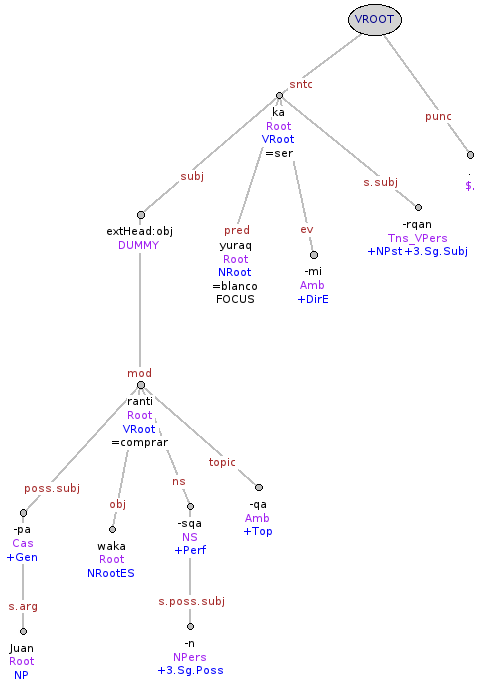
\includegraphics[width=12cm]{tredIHRC.png}
}}
\end{center}
\caption{Frase relativa con cabeza interna (objeto)}\label{Fig:relclauseIntHead}
\end{figure}

\begin{figure}

 \begin{center}
\fbox{
\parbox{10cm}{
\centering \vspace{0.5cm}
{\em \small \~Nuqaq llaqta tiyasqayqa hatun.}\\ \vspace{0.5cm}
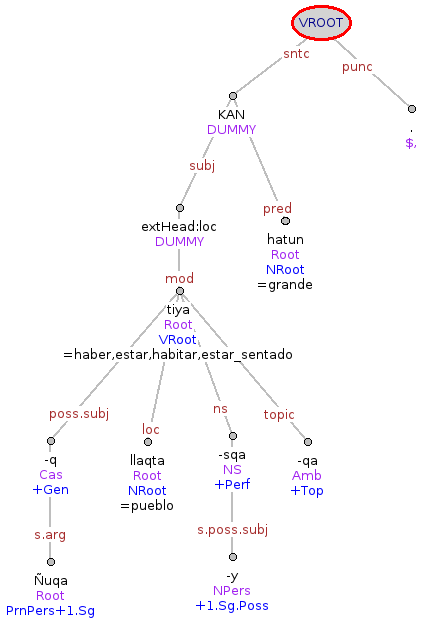
\includegraphics[width=10cm]{tredIHRC2.png}
}}
\end{center}
\caption{Frase relativa con cabeza interna (modificador locativo)}\label{Fig:relclauseIntHead2}
\end{figure}

POVISORIO: (ninguna soluci\'on todav\'ia) 'case float', formas que no se aceptan en todos los idiolectos del Cuzque\~no (?)
\begin{examples}
 \item {\em Warma rikusqayta hamunqa. (?)}
  \item {\em Rikusqay warmata hamunqa. (?)}
\item {\em Rikusqayta warma hamunqa. (?)}
\item {\em rikusqay warma hamunqa.}
\item[] 'La ni\~na que vi va a venir.'\\
 	\hfill{\small \citep[100]{Hastings04}}

\end{examples}

\subparagraph{Frases relativas sin cabeza}

Frases relativas sin cabeza no requieren una cabeza artificial ('dummy'), dependen directamente de su cabeza (p.e. el verbo finito). Recibe la etiqueta seg\'un la relaci\'on con la cabeza.
V\'ease la anotaci\'on del ejemplo \ref{Ex:headless} en Fig. \ref{Fig:headless}. La frase relativa sin cabeza {\em yanapaqniyki} ('los que te ayudan') depende directamente del verbo {\em hamunku} como 'subj'.

\begin{examples}
 \item {\em Llapan \textbf{yachaqkunan} yuyaymananku yuyaysapa kasqanku.}\\
	'All students think (they) are intelligent.'\\
	 'Todos los estudiantes ('los que saben') piensan que son inteligentes.'\\
	  	\hfill{\small \citep[25]{Sanchez2010}}
 \item\label{Ex:headless} {\em ..\textbf{yanapaqniyki} hamunku..} \\
      '..[estos paisanos que] vienen a ayudarte..'\\
      (lit. los que te ayudan, vienen)\\
       	\hfill{\small \citep{Valderrama77}}
\end{examples}

Casos especiales:

\begin{enumerate}
 \item  N\'umeros ordinales con {\em kaq}, v \'ease el ejemplo \ref{Ex:numordKaq} en p\'arrafo \ref{Sec:numord}.
  \item  La combinaci\'on {\em huq kaq} ('otro'): se trata de una frase relativa sin cabeza, {\em huq} es 'pred' de {\em kaq}, y \'este depende del sustantivo que modifica como 'mod'.
 \item  Frase relativa sin cabeza como cabeza interna de otra frase relativa. V\'ease el ejemplo \ref{Ex:specialRel}: La frase relativa sin cabeza {\em chay suwaq} ('ese que roba') es el sujeto de la segunda frase relativa {\em ima suwakusqantapas} ('que roba de todo'), y al mismo tiempo es la cabeza de esta segunda frase relativa. V\'ease la anotaci\'on de este ejemplo en Fig. \ref{Fig:specialRel}.
\end{enumerate}

\begin{examples}
 \item\label{Ex:specialRel} {\em Mariya riqsinchu \textcolor{MidnightBlue}{[}\textcolor{Orchid}{[chay suwaq]} \textcolor{MidnightBlue}{ima suwakusqantapas]}?}\\
      'Does Mariya know the thief that steals anything?'\\
      '{\textquestiondown}Mariya conoce al ladr\'on ('al que roba') que roba cualquier cosa?'
\end{examples}


\begin{figure}

 \begin{center}
\fbox{
\parbox{7cm}{
\centering \vspace{0.5cm}
{\em \small ..yanapaqniyki hamunku..}\\ \vspace{0.5cm}
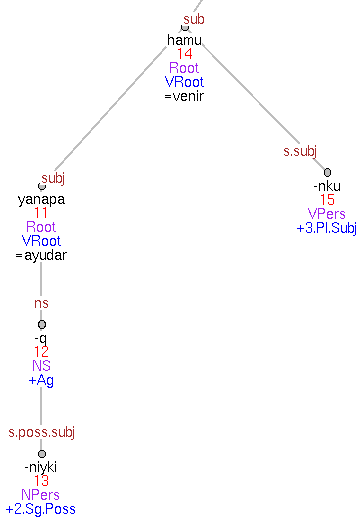
\includegraphics[width=7cm]{tred48.png}
}}
\end{center}
\caption{Frase relativa sin cabeza}\label{Fig:headless}
\end{figure}

\begin{figure}
\begin{center}\fbox{
 \begin{tikzpicture}
   \draw (0,1) node (text) {\small{\em Mariya riqsinchu \textcolor{MidnightBlue}{[}\textcolor{Orchid}{[chay suwaq]} \textcolor{MidnightBlue}{ima suwakusqantapas]}?}};
     \draw (0,0) node (riqsi) {riqsi};
   \draw (-3,-2) node (Mariya) {Mariya};
         \draw (-3,-4) node (-qa) {-qa};
   \draw (0,-2) node (-n) {-n};
   \draw (2,-2) node (-chu) {-chu};
   \draw (4,-2) node (-ta) {\textcolor{MidnightBlue}{-ta}};
   \draw (4,-3) node (extHead) {\textcolor{MidnightBlue}{extHead:subj}};
   
   \draw (4,-4) node (suwa) {\textcolor{MidnightBlue}{suwa}};
   \draw (6,-6) node (-ku) {\textcolor{MidnightBlue}{-ku}};
   \draw (8,-5) node (-sqa) {\textcolor{MidnightBlue}{-sqa}};
      \draw (8,-7) node (-n2) {\textcolor{MidnightBlue}{-n}};
   \draw (11,-5) node (-pas) {\textcolor{MidnightBlue}{-pas}};  
   \draw (4,-6) node (ima) {\textcolor{MidnightBlue}{ima}};
   
   \draw (2,-5) node (suwa2) {\textcolor{Orchid}{suwa}};
      \draw (3,-7) node (-q) {\textcolor{Orchid}{-q}};
      \draw (1,-7) node (chay) {\textcolor{Orchid}{chay}};

       \path[-] (Mariya) edge  node[label=left:$subj$] {} (riqsi);
	       \path[-] (-qa) edge  node[label=left:$topic$] {} (Mariya);
        \path[-] (-n) edge  node[label=left:$s.subj$] {} (riqsi);
        \path[-] (-chu) edge  node[label=right:$intr$] {} (riqsi);
        \path[-,color=MidnightBlue] (-ta) edge  node[label=right:\textcolor{MidnightBlue}{$obj$}] {} (riqsi);        
        
        \path[-,color=MidnightBlue] (extHead) edge  node[label=right:\textcolor{MidnightBlue}{$s.arg$}] {} (-ta);
        \path[-,color=MidnightBlue] (suwa) edge  node[label=right:\textcolor{MidnightBlue}{$mod$}] {} (extHead);
        \path[-,color=MidnightBlue] (-ku) edge  node[label=right:\textcolor{MidnightBlue}{$mod$}] {} (suwa);
        \path[-,color=MidnightBlue] (-sqa) edge  node[label=right:\textcolor{MidnightBlue}{$ns$}] {} (suwa);
	    \path[-,color=MidnightBlue] (-n2) edge  node[label=right:\textcolor{MidnightBlue}{$s.poss.subj$}] {} (-sqa);
	\path[-,color=MidnightBlue] (-pas) edge  node[label=right:\textcolor{MidnightBlue}{$s.co$}] {} (suwa);
	\path[-,color=MidnightBlue] (ima) edge  node[label=left:\textcolor{MidnightBlue}{$obj$}] {} (suwa);
	
	 \path[-,color=Orchid] (suwa2) edge  node[label=left:\textcolor{Orchid}{$subj$}] {} (suwa);
	     \path[-,color=Orchid] (-q) edge  node[label=right:\textcolor{Orchid}{$ns$}] {} (suwa2);
	     \path[-,color=Orchid] (chay) edge  node[label=left:\textcolor{Orchid}{$det$}] {} (suwa2);


\end{tikzpicture}}
\caption{Frase relativa sin cabeza como cabeza interna de otra frase relativa}\label{Fig:specialRel}
\end{center}
\end{figure}

\subsubsection{Formas finitas}\label{Sec:SubFinita}
\paragraph{Oraciones con part\'icula conectiva}
Frases que contienen una oraci\'on finita subordinada por un elemento conectivo como {\em chaymi, chaysi, chayqa, chayri, chaytay} etc. dependen de la cabeza de la primera frase como 'sub'. El elemento conectivo depende de la cabeza de 'su' oraci\'on como 'linker', v\'ease Fig. \ref{Fig:linkersubord} con la anotaci\'on del ejemplo \ref{Ex:linkersubord}.

\begin{examples}
 \item\label{Ex:linkersubord} {\em Phawanchis chaymi, llukulla purinchis.}\\
	'Cuando corremos, avanzamos r\'apido.'
  \item {\em Hamunqa chay\~nay\'a, tapusaq.}\\
	'Pues, ya cuando \'el venga le preguntar\'e al respecto.'
 \item {\em Karupin wasinku (kashan), chayqa chayraqch\'a rikhurimunqaku.}\\
	'La casa de ellos est\'a lejos, por consiguiente aparecer\'an reci\'en.\\
  	\hfill{\small \citep[264-266]{Cusi2}}
\end{examples}


\begin{figure}
\begin{center}\fbox{
 \begin{tikzpicture}
   \draw (0,1) node (text) {\small{\em Phawanchis chaymi, llukulla purinchis.}};
     \draw (0,0) node (puri) {puri};
   \draw (-3,-2) node (Phawa) {Phawa};
         \draw (-3,-4) node (-nchis2) {-nchis};
         \draw (-1,-4) node (chaymi) {chaymi};
   \draw (1,-2) node (llukulla) {llukulla};
   \draw (3,-2) node (-nchis) {-nchis};

      \path[-,color=blue] (Phawa) edge  node[label=left:\textcolor{blue}{$sub$}] {} (puri);
      \path[-] (-nchis2) edge  node[label=left:$s.subj$] {} (Phawa);
      \path[-,color=blue] (chaymi) edge  node[label=right:\textcolor{blue}{$linker$}] {} (Phawa);
      \path[-] (llukulla) edge  node[label=left:$mod$] {} (puri);
      \path[-] (-nchis) edge  node[label=right:$s.subj$] {} (puri);

\end{tikzpicture}}
\caption{Subordinaci\'on de una oraci\'on finita}\label{Fig:linkersubord}
\end{center}
\end{figure}

\paragraph{Oraciones directas}
Oraciones directas dependen del 'verbum dicendi' ({\em niy, rimay} etc.) como 'quot' ('quotation'). Si {\em niy} se presenta como {\em nispa} m\'as una forma finita (p.e. {\em nispa nin}), la forma finita es la cabeza, {\em nispa} depende de ella como 'sub' y la oraci\'on directa depende de {\em nispa} como 'quot'.

\begin{examples}
 \item {\em Ninku ``suwakunas \~nak'aqmanta pasachikuspa purinkuman'' nispa.}\\
	'Y hablan ``Dice que podr\'ian ser los ladrones que andan simulando ser pistacos''.'
 \item {\em Chayta mancharikunku ``\~nak'aqch\'a phawayamuwashan'' nispa.}\\
      'Y de eso se asustan, diciendo ``{\textexclamdown}Oh, seguramente ser\'a el pistaco aqu\'el que se me est\'a acercando!''.'\\
  	\hfill{\small \citep[267]{Cusi2}}
  
\end{examples}

V\'ease Fig. \ref{Fig:nispa}, y tambi\'en Fig. \ref{Fig:nispa2} para una ilustraci\'on.

\begin{figure}

 \begin{center}
\fbox{
\parbox{10cm}{
\centering \vspace{0.5cm}
{\em \small Manan puriyta atinmanchu, nispa.}\\ \vspace{0.5cm}
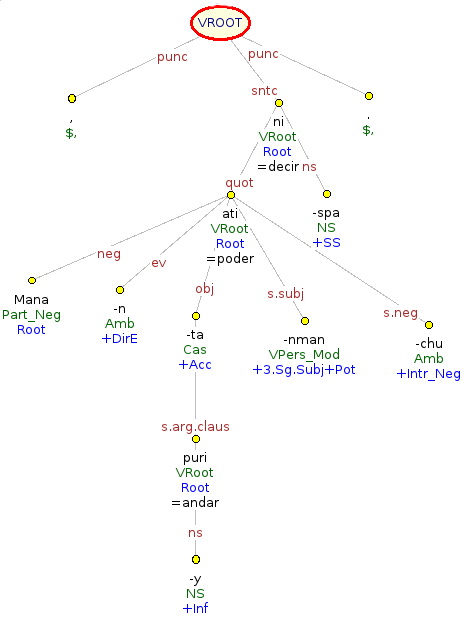
\includegraphics[width=10cm]{tred35.png}
}}
\end{center}
\caption{Oraci\'on directa ({\em nispa})}\label{Fig:nispa}
\end{figure}


\begin{figure}
\begin{center}\fbox{
 \begin{tikzpicture}
\draw (-6,1.5) node (text) {\small{\em Ninku ``suwakunas \~nak'aqmanta pasachikuspa purinkuman'' nispa.}};
     \draw (-12,0) node (Ni) {Ni};
        \draw (-11,-2) node (-nku) {-nku};
        \draw (-1,-2) node (ni) {ni};
             \draw (0,-4) node (-spa) {-spa};
	      \draw (-2,-4) node (puri) {puri};
                    \draw (-1,-6) node (-nkuman) {-nkuman};
                    \draw (-6,-6) node (pasa) {pasa};
                         \draw (-5,-9) node (-chi) {-chi};
                         \draw (-3.5,-10) node (-ku) {-ku};
                         \draw (-3,-8) node (-spa2) {-spa};
                             \draw (-7,-9) node (-manta) {-manta};
                                  \draw (-7,-11) node (nakhaq) {\~nakaq};
                             \draw (-10,-9) node (suwakuna) {suwakuna};
				  \draw (-10,-9.5) node (FOCUS) {{\scriptsize (FOCUS)}};
                             \draw (-8,-9) node (-s) {-s};

% 
%       \path[-,color=blue] (Phawa) edge  node[label=left:\textcolor{blue}{$sub$}] {} (puri);
       \path[-] (-s) edge  node[label=left:$ev$] {} (pasa);
       \path[-] (suwakuna) edge  node[label=left:$subj$] {} (pasa);
       \path[-] (-manta) edge  node[label=right:$mod$] {} (pasa);
           \path[-] (nakhaq) edge  node[label=right:$s.arg$] {} (-manta);
       \path[-] (-spa2) edge  node[label=right:$ns$] {} (pasa);
       \path[-] (-ku) edge  node[label=right:$mod$] {} (pasa);
       \path[-] (-chi) edge  node[label=right:$mod$] {} (pasa);

       \path[-] (-nkuman) edge  node[label=right:$s.subj$] {} (puri);
       \path[-] (pasa) edge  node[label=above:$sub$] {} (puri);

       \path[-] (-spa) edge  node[label=right:$ns$] {} (ni);
       \path[-,color=blue] (puri) edge  node[label=left:\textcolor{blue}{$quot$}] {} (ni);

       \path[-] (-nku) edge  node[label=right:$s.subj$] {} (Ni);
       \path[-,color=blue] (ni) edge  node[label=above:\textcolor{blue}{$sub$}] {} (Ni);


\end{tikzpicture}}
\caption{Oraci\'on directa ({\em nispa ninku})}\label{Fig:nispa2}
\end{center}
\end{figure}

\subsubsection{Oraciones directas sin 'verbum dicendi'}

Ya que anotamos s\'olo a nivel de frases, una secuencia de oraciones directas se divide en varias frases para anotar. En este caso es posible tener una oraci\'on directa sin 'verbum dicendi'. Aqui hay dos opciones: Si la oraci\'on directa es una frase completa, recibe la etiqueta 'sntc', pero si no es una oraci\'on completa, recibe la etiqueta 'quot'. V\'ease el ejemplo \ref{Ex:VROOTquot1}: La oraci\'on principal es {\em Paytaqmi niwaranku:}, entonces la primera oraci\'on directa {\em -Ama hereje kaychischu, carajo!} depende de ella como 'quot'. En cambio,la segunda oraci\'on {\em Ya! Cuatro \'ultimos, a formarse!} (no apartamos el {\em Ya!}) es una frase aparte, pero no es una oraci\'on completa y le falta la cabeza {\em niwaranku}.
Por lo tanto, recibe el label 'quot' en vez de 'sntc', v\'ease la anotaci\'on en Fig. \ref{Fig:VROOTquot1}.\\
La segunda oraci\'on directa del ejemplo \ref{Ex:VROOTquot2} en cambio es una oraci\'on completa: {\em Kay mañosoqa kutiramusqamá; seguro riki mana rakrana kamunchu}. En este caso, recibe la etiqueta 'sntc', v\'ease la anotaci\'on en Fig. \ref{Fig:VROOTquot2}.\\
De hecho, el ejemplo \ref{Ex:VROOTquot2} contiene otro caso de oraciones directas sin 'verbum dicendi': {\em A carajo} depende directamente de {\em rikuruwasqapuni}, ya que {\em nispa} falta (elisi\'on). 
\begin{examples}
 \item\label{Ex:VROOTquot1} {\em Paytaqmi niwaranku: -Ama hereje kaychischu, carajo! Ya! Cuatro \'ultimos, formarse!}\\
    Y \'el nos respondi\'o: -No sean herejes, {\textexclamdown}carajo! {\textexclamdown}Ya Cuatro \'ultimos! formarse.
  \item\label{Ex:VROOTquot2}  {\em Pero hinawanpas chay desalmadoqa rikuruwasqapuni: A carajo! Kay mañosoqa kutiramusqamá; seguro riki mana rakrana kamunchu.}\\
	Pero este desalmado siempre me vio: -Ah ¡carajo! Este mañoso había regresado; seguro le ha faltado tragadera.                                             
\end{examples}

\begin{figure}
 \begin{center}
\fbox{
\parbox{\textwidth}{
\centering \vspace{0.5cm}
{\em \small Paytaqmi niwaranku: -Ama hereje kaychischu, carajo! Ya! Cuatro \'ultimos, formarse!}\\ \vspace{0.5cm}
 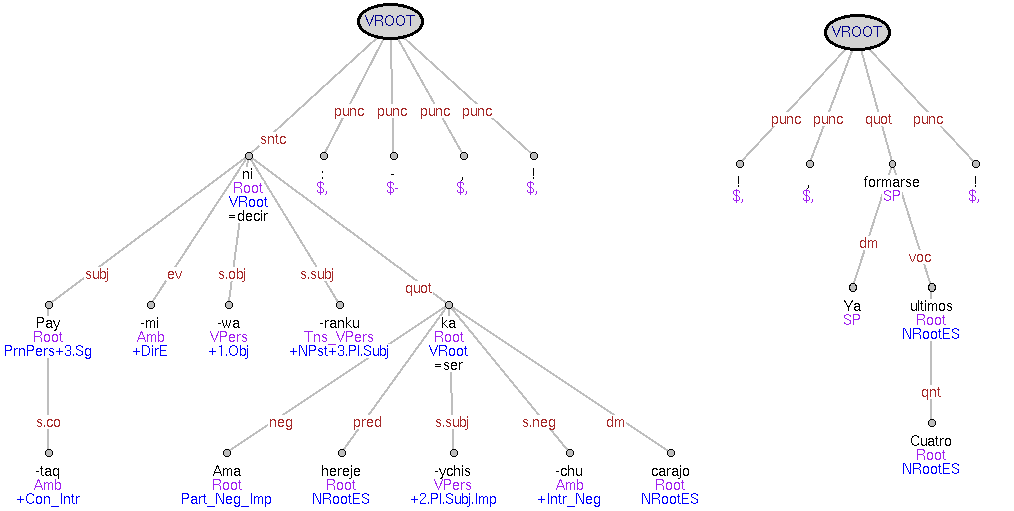
\includegraphics[width=\textwidth]{tred44.png}
}}
\end{center}
\caption{Oraci\'on directa sin 'verbum dicendi', no completa}\label{Fig:VROOTquot1}
\end{figure}

\begin{figure}
 \begin{center}
\fbox{
\parbox{\textwidth}{
\centering \vspace{0.5cm}
{\em \small Pero hinawanpas chay desalmadoqa rikuruwasqapuni: A carajo! Kay mañosoqa kutiramusqamá; seguro riki mana rakrana kamunchu.}\\ \vspace{0.5cm}
 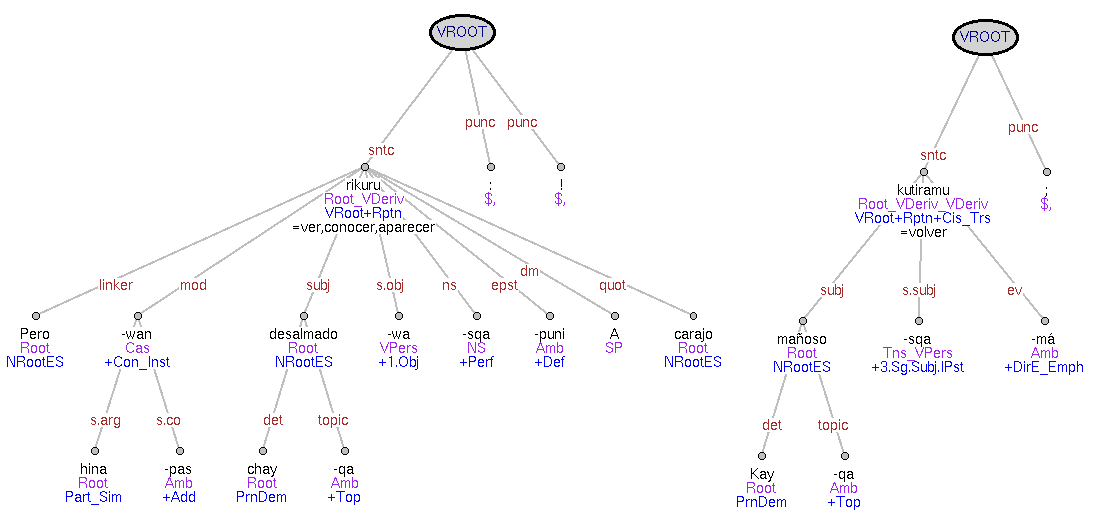
\includegraphics[width=\textwidth]{tred47.png}
}}
\end{center}
\caption{Oraci\'on directa sin 'verbum dicendi', completa}\label{Fig:VROOTquot2}
\end{figure}




\subsection{Oraciones incrustadas}\label{Sec:incrustada}

Oraciones finitas incrustadas que se 'resumen' con un pronombre demonstrativo que lleva el sufijo de caso correspondiente, dependen de este pronombre con la etiqueta 'rep' ('repeated element').

\begin{examples}
 \item\label{Ex:incrustada} {\em Tapuylla tapurikuy [maymantacha kani] chayta.}\\
      'Si fuera posible, averigua no m\'as acerca de cu\'al es el lugar de mi procedencia.'
 \item {\em Chaypi wachachaqa allinta yupaykun [llapanchus uwihakuna hampuran icha mayqinchus qhipakamuranpis] chayta.}\\
      'Y all\'i la chiquilla recuenta atentamente, para saber si todas las ovejas han venido o es que se han quedado algunas (en el campo).'\\
  	\hfill{\small \citep[266-267]{Cusi2}}
\end{examples}

V\'ease Fig. \ref{Fig:incrustada} con la anotaci\'on del ejemplo \ref{Ex:incrustada}.

\begin{figure}
\begin{center}\fbox{
 \begin{tikzpicture}[scale=0.7]
     \draw (2,1) node (text) {{\em \small Tapuylla tapurikuy maymantacha kani chayta.}};
     \draw (0,0) node (tapuri) {tapuri};
        \draw (0,-2) node (-ku) {-ku};
        \draw (2,-3) node (-y) {-y};
         \draw (-3,-2) node (tapu) {tapu};
            \draw (-2,-4) node (-y2) {-y};
            \draw (-1,-4) node (-lla) {-lla};
         \draw (8,-4) node (-ta) {-ta};
            \draw (8,-6) node (chay) {chay};

                 \draw (3,-10) node (-manta) {-manta};
                 \draw (3,-12) node (may) {may};
                 \draw (5,-10) node (-cha) {-cha};
                 \draw (6,-8) node (ka) {ka};
                 \draw (7,-10) node (-ni) {-ni};

       \path[-,color=blue] (ka) edge  node[label=left:\textcolor{blue}{$rep$}] {} (chay);
       \path[-] (may) edge  node[label=left:$s.arg$] {} (-manta);
       \path[-] (-manta) edge  node[label=left:$pred$] {} (ka);
       \path[-] (-cha) edge  node[label=right:$ev$] {} (ka);
       \path[-] (-ni) edge  node[label=right:$s.subj$] {} (ka);

       \path[-] (chay) edge  node[label=right:$s.arg$] {} (-ta);
       \path[-] (-ta) edge  node[label=right:$obj$] {} (tapuri);
       \path[-] (-ku) edge  node[label=left:$mod$] {} (tapuri);
       \path[-] (-y) edge  node[label=right:$s.subj$] {} (tapuri);
       \path[-] (tapu) edge  node[label=left:$adv$] {} (tapuri);

       \path[-] (-y2) edge  node[label=left:$ns$] {} (tapu);
       \path[-] (-lla) edge  node[label=right:$mod$] {} (tapu);
\end{tikzpicture}}
\caption{Oraci\'on incrustada}\label{Fig:incrustada}
\end{center}
\end{figure}

\subsection{Oraciones con copula}\label{Sec:copula}
\subsubsection{Oraciones existenciales}\label{Sec:kayexist}
En oraciones existenciales la copula es la cabeza y el elemento que 'existe', o que 'hay' se anota como 'subj'. Si hay un elemento predicativo, \'este depende de la copula con la etiqueta 'pred'. V\'ease la anotaci\'on del ejemplo \ref{Ex:kayexist} en Fig. \ref{Fig:kayexist}.

\begin{examples}
 \item {\em Kashanmi t'antaqa.}\\
      'S\'i, hay panes.'
\item\label{Ex:kayexist} {\em Escuelapin nuqaqa kashani.}\\
      'Yo estoy en la escuela.'
  	\hfill{\small \citep[91]{Cusi2}}
\end{examples}

\begin{figure}
\begin{center}\fbox{
 \begin{tikzpicture}
     \draw (0,1) node (ka) {\small{\em Escuelapin nuqaqa kashani.}};
     \draw (0,0) node (ka) {ka};
         \draw (4,-2) node (-shani) {-shani};
         \draw (1,-2) node (nuqa) {nuqa};
            \draw (1,-4) node (-qa) {-qa};
   \draw (-2,-2) node (-pi) {-pi};
	\draw (-2,-2.5) node (FOCUS) {\scriptsize{(FOCUS)}};
   \draw (-2,-4) node (Escuela) {Escuela};
   \draw (-0.5,-2) node (-n) {-n};


       \path[-,color=blue] (-pi) edge  node[label=left:\textcolor{blue}{$pred$}] {} (ka);
       \path[-] (-shani) edge  node[label=right:$s.subj$] {} (ka);
       \path[-] (nuqa) edge  node[label=right:$subj$] {} (ka);
       \path[-] (-n) edge  node[label=left:$ev$] {} (ka);
       \path[-] (-qa) edge  node[label=right:$topic$] {} (nuqa);
       \path[-] (Escuela) edge  node[label=left:$s.arg$] {} (FOCUS);

\end{tikzpicture}}
\caption{Oraci\'on existencial con elemento predicativo}\label{Fig:kayexist}
\end{center}
\end{figure}

\subsubsection{Oraciones ecuacionales}\label{Sec:kayecuacional}
Las oraciones ecuacionales se anota de la misma manera como las oraciones existenciales descritas en p\'arrafo \ref{Sec:kayexist}: La copula es la cabeza, mientras que el elemento predicativo depende de ella como 'pred'.

\begin{examples}
 \item\label{Ex:kayecuacional} {\em Qanqa allin warmin kanki.}\\
      'T\'u eres una buena mujer.'
 \item {\em Hayk'a watayuqtaq kankiri?}\\
      '{\textquestiondown}Y qu\'e edad tienes t\'u?'\\
  	\hfill{\small \citep[91-92]{Cusi2}}
\end{examples}
 
V\'ease Fig. \ref{Fig:kayecuacional} para una ilustraci\'on de la anotaci\'on del ejemplo \ref{Ex:kayecuacional}.
 
\begin{figure}
\begin{center}\fbox{
 \begin{tikzpicture}
     \draw (1,1) node (ka) {\small{\em Qanqa allin warmin kanki.}};
     \draw (1,0) node (ka) {ka};
         \draw (4,-2) node (-nki) {-nki};
         \draw (2,-2) node (-n) {-n};
         \draw (0,-2) node (warmi) {warmi};
	      \draw (0,-2.5) node (FOCUS) {\scriptsize(FOCUS)};
	      \draw (0,-4) node (allin) {allin};
	 \draw (-3,-2) node (Qan) {Qan};
               \draw (-3,-4) node (-qa) {-qa};



       \path[-,color=blue] (warmi) edge  node[label=left:\textcolor{blue}{$pred$}] {} (ka);
       \path[-] (allin) edge  node[label=right:$mod$] {} (FOCUS);
       \path[-] (-qa) edge  node[label=right:$topic$] {} (Qan);
       \path[-] (-n) edge  node[label=right:$ev$] {} (ka);
       \path[-] (-nki) edge  node[label=right:$s.subj$] {} (ka);
       \path[-] (Qan) edge  node[label=left:$subj$] {} (ka);
\end{tikzpicture}}
\caption{Oraci\'on ecuacional con elemento predicativo}\label{Fig:kayecuacional}
\end{center}
\end{figure}

  \subsubsection{Kay como auxiliar}
\paragraph{{\em kanpis} (adem\'as, a\'un, incluso)}

El uso de la forma {\em kanpis} en el sentido de 'adem\'as, a\'un, incluso' es un caso especial: {\em kanpis} depende de la cabeza de la frase como 'mod'.

\begin{examples}
 \item {\em Ruphayamushanmi kanpis.}\\
	'Adem\'as, est\'a soleando.
 \item {\em Paramunqachus kanpis asllatawanqa.}\\
      'De repente va a llover m\'as tarde.\\
 	\hfill{\small \citep[210]{Cusi2}}
\end{examples}

\paragraph{Formas anal\'iticas del verbo}

Las formas del verbo que usan la copula {\em kay} como auxiliar son los siguientes:

\begin{examples}
 \item[]\textbf{pasado habitual:} \\
    \item\label{Ex:kayhabitual} {\em Tinku kaspayqa hatukuytan qatikachakuq kani.}\\ 
	  'Cuando era peque\~no siempre iba con mi abuelo a cualquier parte.'
    \item {\em Yunkapiqa ch'isillanmi kukata pallaq kasqaku.}\\
 	  'En los valles recogen las hojas de la coca, solamente de noche.'
 \item[]\textbf{condicional pasado:}\\
   \item\label{Ex:kaycondicional} {\em Punchayta apakuyman karan chayqa, mana para apiyamuwanmanchu karqan.}\\
	'Si hubiera llevado mi poncho, no me hubiese mojado la lluvia.'
\end{examples}

En el primer caso, el pasado habitual, la copula es la cabeza de la oraci\'on ya que el verbo principal, nominalizado por {\em -q}, no es finito. El verbo principal depende entonces de la copula como 'hab' (habitual).\\
IMPORTANTE: Los argumentos y adjuntos del verbo no finito en {\em -q} dependen de este verbo, no de la copula, con la excepci\'on del sujeto: \'este depende de la copula (la forma finita). Modificadores que modifican a la oraci\'on entera dependen de {\em ka-}, en cambio modificadores que modifican al verbo principal (adjuntos y adverbios) dependen de forma en {\em -q}. La negaci\'on {\em mana ..-chu} y los evidenciales modifican a la oraci\'on entera, as\'i que dependen de {\em ka-} (y si forman parte del verbo en {\em -q}, \'este es FOCUS). Oraciones subordinadas ('sub') normalmente dependen de la oraci\'on entera, as\'i pertenecen a {\em ka-}, no al verbo principal en {\-q}. Elementos coordinadores o subordinadores ('linker') tambi\'en dependen de {\em -ka}.\\
V\'ease Fig. \ref{Fig:kayhabitual} con la anotaci\'on del ejemplo \ref{Ex:kayhabitual}.\\
Una forma especial del pasado habitual son oraciones ecuacionales/existenciales con {\em kaq}: Estas formas requieren el 'dummy element' KAN, as\'i que en este caso hay dos c\'opulas, una finita y otra no finita, v\'ease Fig. \ref{Fig:kaqKAN}.\\ 
En el segundo caso, el condicional pasado, la oraci\'on contiene dos verbos finitos, por lo tanto, el verbo principal es la cabeza y la copula depende de ella como 'aux' (auxiliar). V\'ease tambi\'en Fig. \ref{Fig:kaycondicional} con la anotaci\'on del ejemplo \ref{Ex:kaycondicional}.

\begin{figure}
\begin{center}\fbox{
 \begin{tikzpicture}
   \draw (-4,1) node (text) {\small{\em Tinku kaspayqa hatukuytan qatikachakuq kani.}};
     \draw (0,0) node (ka) {ka};
         \draw (2,-2) node (-ni) {-ni};
         \draw (0,-2) node (qatikacha) {qatikacha};
            \draw (-1,-4) node (-ku) {-ku};
            \draw (1,-4) node (-q) {-q};
            \draw (-5,-4) node (-ta) {-ta};
	      \draw (-5,-4.5) node (FOCUS) {\scriptsize(FOCUS)};
                 \draw (-5,-6) node (hatuku) {hatuku};
                 \draw (-5,-8) node (-y) {-y};
         \draw (-3,-4) node (-n) {-n};


	 \draw (-9,-2) node (ka2) {ka};
 	     \draw (-9,-4) node (-spa) {-spa};
 	           \draw (-9,-6) node (-y2) {-y};
 	     \draw (-7,-4) node (-qa) {-qa};
             \draw (-11,-4) node (Tinku) {Tinku};
 
        \path[-,color=blue] (qatikacha) edge  node[label=right:\textcolor{blue}{$hab$}] {} (ka);
        \path[-] (-ni) edge  node[label=right:$s.subj$] {} (ka);
        \path[-] (-ku) edge  node[label=left:$mod$] {} (qatikacha);
        \path[-] (-q) edge  node[label=right:$ns$] {} (qatikacha);
        \path[-] (-ta) edge  node[label=left:$obj$] {} (qatikacha);
           \path[-] (hatuku) edge  node[label=left:$s.arg$] {} (FOCUS);
	   \path[-] (-y) edge  node[label=left:$s.subj$] {} (hatuku);
        \path[-] (-n) edge  node[label=left:$ev$] {} (ka);

        \path[-] (ka2) edge  node[label=above:$sub$] {} (ka);
           \path[-] (-spa) edge  node[label=right:$ns$] {} (ka2);
               \path[-] (-y2) edge  node[label=right:$s.poss.subj$] {} (-spa);
           \path[-] (Tinku) edge  node[label=left:$pred$] {} (ka2);
           \path[-] (-qa) edge  node[label=right:$topic$] {} (ka2);
\end{tikzpicture}}
\caption{Pasado habitual}\label{Fig:kayhabitual}
\end{center}
\end{figure}

\begin{figure}
\begin{center}\fbox{
 \begin{tikzpicture}[scale=0.9]   
  \draw (-1,1) node (text) {\small{\em Punchayta apakuyman karan chayqa, mana para apiyamuwanmanchu karqan.}};
     \draw (0,0) node (apiyamu) {apiyamu};
         \draw (0,-3) node (-wa) {-wa};
         \draw (2,-3) node (-nman) {-nman};
         \draw (4,-2.5) node (-chu) {-chu};
         \draw (6,-2) node (ka) {ka};
             \draw (6,-4) node (-rqan) {-rqan};
          \draw (-1,-4) node (para) {para};
          \draw (-3,-4) node (mana) {mana};

          \draw (-7,-6) node (apa) {apa};
                \draw (-3,-8) node (chay) {chay};
                     \draw (-3,-10) node (-qa) {-qa};
                \draw (-7,-9) node (-yman) {-yman};
                \draw (-5,-8) node (ka2) {ka};
                    \draw (-5,-10) node (-ran) {-ran};
                \draw (-9,-8) node (-ta) {-ta};
                   \draw (-9,-10) node (Punchu) {Punchu};
                     \draw (-9,-12) node (-y) {-y};

         \path[-,color=blue] (ka) edge  node[label=right:\textcolor{blue}{$aux$}] {} (apiyamu);
         \path[-,color=blue] (ka2) edge  node[label=right:\textcolor{blue}{$aux$}] {} (apa);

         \path[-] (-nman) edge  node[label=right:$s.subj$] {} (apiyamu);
         \path[-] (-wa) edge  node[label=right:$s.obj$] {} (apiyamu);
         \path[-] (-chu) edge  node[label=right:$s.neg$] {} (apiyamu);
            \path[-] (-rqan) edge  node[label=right:$s.subj$] {} (ka);
         \path[-] (mana) edge  node[label=left:$neg$] {} (apiyamu);
         \path[-] (para) edge  node[label=left:$subj$] {} (apiyamu);


         \path[-] (chay) edge  node[label=right:$linker$] {} (apa);
              \path[-] (-qa) edge  node[label=right:$topic$] {} (chay);
 	   \path[-] (-ran) edge  node[label=right:$s.subj$] {} (ka2);
         \path[-] (-yman) edge  node[label=right:$s.subj$] {} (apa);
         \path[-] (-ta) edge  node[label=right:$obj$] {} (apa);
         \path[-] (Punchu) edge  node[label=right:$s.arg$] {} (-ta);
         \path[-] (-y) edge  node[label=right:$s.poss$] {} (Punchu);

         \path[-] (apa) edge  node[label=left:$sub$] {} (apiyamu);
\end{tikzpicture}}
\caption{Condicional pasado}\label{Fig:kaycondicional}
\end{center}
\end{figure}

\begin{figure}
 \begin{center}
\fbox{
\parbox{10cm}{
\centering \vspace{0.5cm}
{\em \small ..manaña ni pacienciapas kaqchu aguantanaqa.}\\ \vspace{0.5cm}
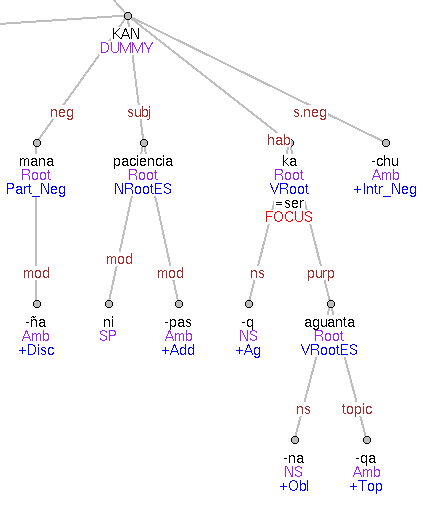
\includegraphics[width=10cm]{tred39.png}
}}
\end{center}
\caption{Pasado habitual con {\em kaq} y 'dummy element'}\label{Fig:kaqKAN}
\end{figure}





\subsubsection{Elisi\'on de c\'opula}
En oraciones ecuacionales o existenciales de tercera persona, que a veces carecen de copula, se inserta un 'dummy element', un nodo que tiene 'KAN' como valor del atributo 'word'. El valor de su atributo 'pos' (part-of-speech) es 'DUMMY'. V\'ease Fig. \ref{Fig:KAN} con la anotaci\'on del ejemplo \ref{Ex:KAN}.

\begin{examples}
 \item {\em Pawluchan wawqiyqa.}\\
      'Mi hermano es Pablito.'\\
 	\hfill{\small \citep[93]{Cusi2}}
 \item\label{Ex:KAN} {\em ..Gregorio Mamanin sutiy.}\\
      '..mi nombre es Gregorio Mamani.'\\
     	\hfill{\small \citep{Valderrama77}}
\end{examples}

V\'ease tambi\'en Fig. \ref{Fig:adverbios} ,\ref{Fig:manadm}, \ref{Fig:aridm} o \ref{Fig:mantasuper} como ejemplos.

\begin{figure}
 \begin{center}
\fbox{
\parbox{6.5cm}{
\centering \vspace{0.5cm}
{\em \small ..Gregorio Mamanin sutiy.}\\ \vspace{0.5cm}
  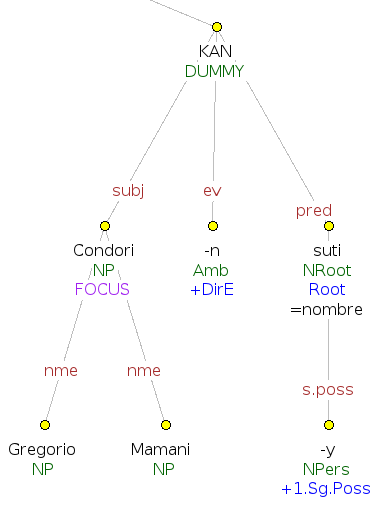
\includegraphics[width=6.5cm]{tred33.png}}}
 \end{center}
\caption{Elisi\'on de copula}\label{Fig:KAN}
\end{figure}



\subsubsection{La construcci\'on..{\em -na + kay} (tener que..)}\label{Sec:nakay}

La construcci\'on de un verbo nominalizado con {\em -na} y una forma finita de la copula se anota de esta manera:
La copula es la cabeza de la frase, y la forma con {\em -na} depende de ella como 'oblg' (obligaci\'on).\\t
OJO: el sujeto puede ser marcado con genitivo o no, siempre depende del verbo nominalizado con {\em -na}, ya que est\'a marcado en ello con un sufijo posesivo (NO depende de la copula, al contrario de las formas habituales con {\em -q}!).

\begin{examples}
 \item {\em Usqhaymi \textbf{rinay} kashan.}\\
      'Tengo que ir r\'apido.'
 \item\label{Ex:nakay} {\em P'achaymi \textbf{t'aqsakunay} kashan.}\\
      'Tengo que lavar mi ropa.'\\
 	\hfill{\small \citep[210]{Cusi2}}
\end{examples}

V\'ease Fig. \ref{Fig:nakay} para una ilustraci\'on del ejemplo \ref{Ex:nakay}.

\begin{figure}
\begin{center}\fbox{
 \begin{tikzpicture}
   \draw (-2,1) node (text) {\small{\em P'achaymi t'aqsakunay kashan.}};
     \draw (0,0) node (ka) {ka};
     \draw (2,-2) node (-shan) {-shan};
   \draw (-3,-2) node (t'aqsa) {t'aqsa};
         \draw (-2,-4) node (-ku) {-ku};
         \draw (1,-4) node (-na) {-na};
         \draw (1,-6) node (-y) {-y};
   \draw (-6,-4) node (p'acha) {p'acha};
      \draw (-6,-4.5) node (FOCUS) {\scriptsize{(FOCUS)}};
      \draw (-6,-6) node (-y2) {-y};
   \draw (-5,-2) node (-mi) {-mi};


       \path[-,color=blue] (t'aqsa) edge  node[label=right:\textcolor{blue}{$oblg$}] {} (ka);
       \path[-] (-shan) edge  node[label=left:$s.subj$] {} (ka);
       \path[-] (-ku) edge  node[label=right:$mod$] {} (t'aqsa);
       \path[-] (-na) edge  node[label=right:$ns$] {} (t'aqsa);
       \path[-] (-y) edge  node[label=right:$s.poss.subj$] {} (-na);
       \path[-] (-y2) edge  node[label=right:$s.poss$] {} (FOCUS);
       \path[-] (p'acha) edge  node[label=right:$obj$] {} (t'aqsa);
       \path[-] (-mi) edge  node[label=left:$ev$] {} (ka);
\end{tikzpicture}}
\caption{La construcci\'on {\em -na + kay}}\label{Fig:nakay}
\end{center}
\end{figure}

\subsubsection{La construcci\'on..{\em -yuq + kay}}\label{Sec:yuqkay}
Esa construcci\'on, que en espa\~nol corresponde a 'tener algo', se anota asi: el sintagma nominal con {\em -yuq} depende como 'pred' de la ra\'iz de la c\'opula (porque es el elemento predicativo en esta construcci\'on), v\'ease Fig. \ref{Fig:yuq}.

\begin{figure}
 \begin{center}
 \fbox{
\parbox{7cm}{
\centering \vspace{0.5cm}
{\em \small ..hallpayuq\~na kanki.}\\ \vspace{0.5cm}
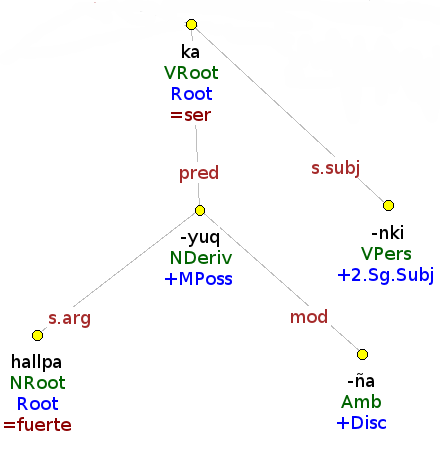
\includegraphics[width=7cm]{tred13.png}}}
\end{center}
\caption{La construcci\'on {\em -yuq + kay}}\label{Fig:yuq}
\end{figure}

\subsection{Oraciones imperativas}
\subsubsection{Imperativos}
Si el hablante se dirige la persona a la que se manda a hacer algo con su nombre, \'este no es se anota como el sujeto (ya que el sujeto es de segunda persona), sino recibe la etiqueta 'voc' (vocative). V\'ease Fig. \ref{Fig:imperativo} para la anotaci\'on del ejemplo \ref{Ex:imperativo}.

\begin{examples}
 \item\label{Ex:imperativo} {\em Yaw Manulcha, unuman riy, qantaq, Margacha, ninata hap'ichiy!}\\
	'Oye Manuelito, anda por agua; y t\'u, Margarita, prende el fuego'\\
 	\hfill{\small \citep[83]{Cusi2}}
 \item {\em Unumansi rinki!}\\
      '{\textexclamdown}Dice que vas a ir por agua!
\end{examples}

\begin{figure}
\begin{center}\fbox{
 \begin{tikzpicture}[scale=0.8]
   \draw (-3.5,1) node (text) {\small{\em Yaw Manulcha, unuman riy, qantaq, Margacha, ninata hap'ichiy!}};
     \draw (0,0) node (hap'i) {hap'i};
       \draw (2,-2) node (-chi) {-chi};
       \draw (5,-2) node (-y) {-y};
       \draw (0.5,-3) node (-ta) {-ta};
           \draw (0.5,-5) node (nina) {nina};
       \draw (-1,-2.5) node (Margacha) {Margacha};
       \draw (-3,-2) node (qan) {qan};
           \draw (-3,-4) node (-taq) {-taq};

    \draw (-8,-2) node (ri) {ri};
    \draw (-6,-4) node (-y2) {-y};
    \draw (-8.5,-4.5) node (-man) {-man};
       \draw (-8.5,-6.5) node (unu) {unu};
    \draw (-11,-4.5) node (Manulcha) {Manulcha};
    \draw (-14,-4) node (Yaw) {Yaw};
% 
        \path[-,color=blue] (Manulcha) edge  node[label=left:\textcolor{blue}{$voc$}] {} (ri);
        \path[-,color=blue] (Margacha) edge  node[label=left:\textcolor{blue}{$voc$}] {} (hap'i);

        \path[-] (-chi) edge  node[label=right:$mod$] {} (hap'i);
        \path[-] (-y) edge  node[label=right:$s.subj$] {} (hap'i);
        \path[-] (-ta) edge  node[label=right:$obj$] {} (hap'i);
		    \path[-] (nina) edge  node[label=right:$s.arg$] {} (-ta);
        \path[-] (qan) edge  node[label=left:$subj$] {} (hap'i);
	            \path[-] (-taq) edge  node[label=left:$s.co$] {} (qan);

        \path[-] (-y2) edge  node[label=right:$s.subj$] {} (ri);
        \path[-] (-man) edge  node[label=right:$goal$] {} (ri);
		\path[-] (unu) edge  node[label=right:$s.arg$] {} (-man);
        \path[-] (Yaw) edge  node[label=above:$dm$] {} (ri);

        \path[-] (ri) edge  node[label=above:$co$] {} (hap'i);
\end{tikzpicture}}
\caption{Imperativo}\label{Fig:imperativo}
\end{center}
\end{figure}
\subsubsection{Exhortativo}
Como exhorativo se entiende el imperativo de la primera persona plural. Si el hablante se dirige con nombres a las personas a quienes invita a hacer algo, \'estas dependen del verbo como 'voc', no como 'subj', v\'ease tambi\'en Fig. \ref{Fig:imperativo}.

\begin{examples}
 \item {\em llamkasun} (Ayacuchano)\\
	'{\textexclamdown}Trabajemos!'\\
 	\hfill{\small \citep[50]{Dedenbach02}}
 \item {\em Haku samapusunchis!}\\
	'{\textexclamdown}Descansemos!\\
 	\hfill{\small \citep[255]{Cusi2}}
\end{examples}

\subsubsection{Jusivo ('jussive')}
El jusivo, o 'imperativo de tercera persona', se anota como una frase declarativa. Si el hablante nombra expl\'icitamente  a las personas quienes deben de hacer algo, el nombre (o los nombres) dependen del verbo como 'subj' (ya que en este caso, el sujeto del verbo es de tercera persona). V\'ease Fig. \ref{Fig:jusivo} con la anotaci\'on del ejemplo \ref{Ex:jusivo}.

\begin{examples}
 \item\label{Ex:jusivo} {\em Kawsachun Tupaq Amaru!}\\
      '{\textexclamdown}Viva T\'upac Amaru!'
 \item {\em Llapan runakuna hamuchunku!}\\
      '{\textexclamdown}Que vengan todos los hombres!'
 	\hfill{\small \citep[255]{Cusi2}}
\end{examples}

\begin{figure}
\begin{center}\fbox{
 \begin{tikzpicture}
   \draw (0,1) node (text) {\small{\em Kawsachun Tupaq Amaru!}};
     \draw (0,0) node (Kawsa) {Kawsa};
         \draw (2,-2) node (-chun) {-chun};
         \draw (-2,-2) node (Amaru) {Amaru};
	      \draw (-2,-4) node (Tupaq) {Tupaq};




       \path[-,color=blue] (Amaru) edge  node[label=left:\textcolor{blue}{$subj$}] {} (Kawsa);
       \path[-] (-chun) edge  node[label=right:$s.subj$] {} (Kawsa);
       \path[-] (Tupaq) edge  node[label=left:$nme$] {} (Amaru);
\end{tikzpicture}}
\caption{Jusivo (imperativo de tercera persona)}\label{Fig:jusivo}
\end{center}
\end{figure}

\section{Construcciones especiales}
\subsection{Extranjerismos y {\em nisqa}}
PROVISORIO (o mejor subsumir todo material no-quechua bajo un nodo no-terminal?)\\
Extranjerismos que se incrustan mediante {\em nisqa} dependen de \'este como 'flm' ('foreign language material'). La estructura interna de las frases extranjeras se anotan (las dependencias), pero las relaciones se dejan sin especificar (la etiqueta es: '$--$'). V\'ease tambi\'en Fig. \ref{Fig:abbrev} como ejemplo.




\subsection{Comparaci\'on}\label{Sec:comparacion}
PROVISORIO (Comparaciones tambi\'en posible con {\em -niray, -rikuq}, tratarlos igual como {\em hina}?)

\subparagraph{Positivo ({\em hina})}

En comparaciones con {\em hina}, sea escrito como sufijo o como posposici\'on, se anota {\em hina} como cabeza del sintagma nominal, \'este depende de {\em hina} como 's.arg' (si {\em hina} es un sufijo) o como 'p.arg' (si {\em hina} es una posposici\'on), {\em hina} depende de su cabeza (la calidad que se compara) como 'comp'. V\'ease la anotaci\'on del ejemplo \ref{Ex:hinacomp} en Fig. \ref{Fig:hinacomp}.

\begin{examples}
 \item\label{Ex:hinacomp} {\em Qaqa hina kapkam kay tantaqa.} (Ayacuchano)\\
      'Este pan es m\'as duro que roca.'
 \item {\em Ramonqa Pedro hina hatunmi.}\\
      'Ramon es tan grande como Pedro.'\\
	\hfill{\small \citep[189-190]{Dedenbach02}}
\end{examples}

\begin{figure}
\begin{center}\fbox{
 \begin{tikzpicture}
   \draw (-1,1) node (text) {\small{\em Qaqa hina kapkam kay tantaqa.}};
     \draw (0,0) node (KAN) {KAN};
             \draw (0,-.5) node (DUMMY) {\scriptsize{(DUMMY)}};
         \draw (-1,-2) node (-m) {-m};
	 \draw (2,-2) node (tanta) {tanta};
	       \draw (3,-4) node (-qa) {-qa};
	       \draw (1,-4) node (kay) {kay};
         \draw (-4,-2) node (kapka) {kapka};
               \draw (-4,-2.5) node (FOCUS) {{\scriptsize(FOCUS)}};
		\draw (-4,-4) node (hina) {\textcolor{blue}{hina}};
               \draw (-4,-6) node (Qaqa) {Qaqa};


         \path[-,color=blue] (hina) edge  node[label=left:\textcolor{blue}{$comp$}] {} (FOCUS);
        \path[-] (tanta) edge  node[label=right:$subj$] {} (DUMMY);
        \path[-] (kapka) edge  node[label=above:$pred$] {} (DUMMY);
        \path[-] (-m) edge  node[label=right:$ev$] {} (DUMMY);
       \path[-] (Qaqa) edge  node[label=left:$p.arg$] {} (hina);
       \path[-] (-qa) edge  node[label=right:$topic$] {} (tanta);
       \path[-] (kay) edge  node[label=left:$det$] {} (tanta);

\end{tikzpicture}}
\caption{Positivo con {\em hina}}\label{Fig:hinacomp}
\end{center}
\end{figure}

\subparagraph{Comparativo ({\em -manta})}

El uso de {\em -manta} en comparativos de la estructura:\\
'{\em [cosa que se compara]} (sujeto) + {\em [cosa con la que se compara]-manta} + {\em aswan/pisi} + {\em[calidad]}'\\
se anota con la etiqueta 'comp' ('comparative') y depende de la calidad en comparaci\'on. V\'ease la anotaci\'on del ejemplo \ref{Ex:mantacomp} en Fig. \ref{Fig:mantacomp}.

\begin{examples}
 \item {\em Qaqamanta aswan kapkam kay tantaqa.} (Ayacuchano)\\
      'Este pan es m\'as duro que roca.'
 \item\label{Ex:mantacomp} {\em Llamakunamanta pisi hatunmi allqukunaqa kanku.}\\
      'Perros son menos grande que llamas.'
 \item {\em Quwikunaqa llamakunamanta aswan pisi hatunmi kanku.}\\
      'Cuys son mucho m\'as chiquitos (mucho menos grande) que llamas.'\\
	\hfill{\small \citep[189-190]{Dedenbach02}}
\end{examples}

\begin{figure}
\begin{center}\fbox{
 \begin{tikzpicture}
   \draw (-3,1) node (text) {\small{\em Llamakunamanta pisi hatunmi allqukunaqa kanku.}};
     \draw (0,0) node (ka) {ka};
         \draw (2,-2) node (-nku) {-nku};
         \draw (-0.5,-2) node (allqukuna) {allqukuna};
	      \draw (-0.5,-4) node (-qa) {-qa};
         \draw (-2.5,-2) node (-mi) {-mi};

         \draw (-4,-2) node (hatun) {hatun};
               \draw (-4,-2.5) node (FOCUS) {{\scriptsize(FOCUS)}};
	       \draw (-4,-4) node (pisi) {pisi};
         \draw (-6,-4) node (-manta) {\textcolor{blue}{-manta}};
               \draw (-6,-6) node (llamakuna) {llamakuna};

        \path[-,color=blue] (-manta) edge  node[label=left:\textcolor{blue}{$comp$}] {} (FOCUS);
        \path[-] (-nku) edge  node[label=right:$s.subj$] {} (ka);
        \path[-] (allqukuna) edge  node[label=right:$subj$] {} (ka);
        \path[-] (hatun) edge  node[label=left:$pred$] {} (ka);
        \path[-] (-mi) edge  node[label=right:$ev$] {} (ka);
       \path[-] (llamakuna) edge  node[label=right:$s.arg$] {} (-manta);
       \path[-] (pisi) edge  node[label=right:$mod$] {} (FOCUS);
        \path[-] (-qa) edge  node[label=right:$topic$] {} (allqukuna);


\end{tikzpicture}}
\caption{Comparativo con {\em -manta}}\label{Fig:mantacomp}
\end{center}
\end{figure}

\subparagraph{Superlativo}

El superlativo se anota de la misma forma como el comparativo, v\'ease la anotaci\'on del ejemplo \ref{Ex:mantasuper} en Fig. \ref{Fig:mantasuper}. Acerca de la Fig. \ref{Fig:mantasuper}: 'KAN' es un 'dummy element', que se inserta en frases d\'onde la c\'opula (3{\textordfeminine} persona singular) se ha omitido. Ya que anotamos dependencias, necesitamos una cabeza en la frase. Notase tambi\'en que el elemento predicativo en oraciones copulativas NO es el verbo auxiliar, sino el sintagma nominal que constituye 'lo que es'. Para m\'as informaci\'on acerca de oraciones con c\'opula, v\'ease tambi\'en p\'arrafo \ref{Sec:copula}.) 

\begin{examples}
 \item {\em Kay sachaqa lliwmanta hatunninmi.} (Ayacuchano)\\
      o: {\em Kay sachaqa lliwmanta hatunnin kaqmi.}\\
      'Este \'arbol es el m\'as grande de todos.'
 \item\label{Ex:mantasuper} {\em Husiyqa lliwmanta aswan pisi hatunmi.} (Ayacuchano)\\
      o: {\em Husiyqa lliwmanta aswan pisi hatunninmi.} \\
      'Jos\'e es el m\'as peque\~no (de todos).'\\
	\hfill{\small \citep[189-190]{Dedenbach02}}
\end{examples}

\begin{figure}
\begin{center}\fbox{
 \begin{tikzpicture}
   \draw (-2.5,1) node (text) {\small{\em Husiyqa lliwmanta aswan pisi hatunninmi.}};
     \draw (0,0) node (KAN) {KAN};
             \draw (0,-.5) node (DUMMY) {\scriptsize(DUMMY)};
         \draw (2,-2.5) node (-mi) {-mi};
	 \draw (-1,-2) node (hatun) {hatun};
               \draw (-1,-2.5) node (FOCUS) {{\scriptsize(FOCUS)}};
	       \draw (0,-4) node (-nin) {-nin};
               \draw (-2,-4) node (pisi) {pisi};
               \draw (-2,-6) node (aswan) {aswan};
         \draw (-4,-4) node (-manta) {\textcolor{blue}{-manta}};
               \draw (-4,-6) node (lliw) {lliw};
         \draw (-6,-2) node (Husiy) {Husiy};
               \draw (-6,-4) node (-qa) {-qa};


         \path[-,color=blue] (-manta) edge  node[label=left:\textcolor{blue}{$comp$}] {} (FOCUS);
        \path[-] (Husiy) edge  node[label=above:$subj$] {} (DUMMY);
        \path[-] (hatun) edge  node[label=right:$pred$] {} (DUMMY);
        \path[-] (-mi) edge  node[label=right:$ev$] {} (DUMMY);
       \path[-] (lliw) edge  node[label=left:$s.arg$] {} (-manta);
       \path[-] (pisi) edge  node[label=left:$mod$] {} (FOCUS);
       \path[-] (-nin) edge  node[label=right:$s.poss$] {} (FOCUS);
       \path[-] (aswan) edge  node[label=left:$mod$] {} (pisi);
        \path[-] (-qa) edge  node[label=left:$topic$] {} (Husiy);


\end{tikzpicture}}
\caption{Superlativo con {\em -manta}}\label{Fig:mantasuper}
\end{center}
\end{figure}

\subsection{Dislocation}\label{Sec:disl}

PROVISORIO: Dislocaciones dependen del verbo como 'r.disl' ('right dislocation',derecha) o 'l.disl' ('left dislocation', izquierda'). 

\begin{examples}
\item[] izquierda:
 \item {\em Hatunpuralla\textbf{ta}m papa\textbf{ta}qa munani.} (Ayacuchano)\\
	'Quiero s\'olo papas grandes.'\\
  	\hfill{\small \citep[80]{Soto76a}}
 \item[] derecha:
 \item {\em Paraqayta\textbf{chu} ichari uwinata\textbf{chu} munashanki sarata\textbf{ri}?}\\
      '{\textquestiondown}Deseas la calidad blanca o la amarilla del ma\'iz?'\\
    		\hfill{\small \citep[236]{Cusi2}}
\end{examples}

V\'ease los ejemplos en Fig. \ref{Fig:suna} (izquierda) y Fig. \ref{Fig:chucoord} (derecha).

\subsection{La construcci\'on..{\em -q + verbo de movimiento} (ir a/para..)}

La construcci\'on {\em -q} + verbo de movimiento se anota de esta forma: La forma agentiva en {-q} depende del verbo de movimiento como 'purp' (purpose).
\begin{examples}
 \item {\em Qusqutam \textbf{rishani} llank'apaku\textbf{q}.}\\
	'Estoy yendo al Cuzco a conseguirme trabajo.'
\item {\em Chakraytan \textbf{rishani} papa aysa\textbf{q}.}\\
      'Estoy yendo a mi chacra a aporcar la papa.
 	\hfill{\small \citep[209]{Cusi2}}
 \item {\em ..\textbf{pawanpuni} Birnacha kachu\textbf{q}.}\\
      '..[el perro] corre para morder a Birnacha.' \\
 	\hfill{\small \citep[91]{Dedenbach02}}
\end{examples}

\subsection{Aposiciones}
Una aposici\'on es una frase (u oraci\'on) que da una explanaci\'on o una descripci\'on m\'as detallada de algo. Una caracter\'istica especial de aposiciones es que pueden sustituir el sustantivo que modifican, sin que cambie la sem\'antica de la oraci\'on. Por lo tanto, aposiciones siempre llevan el mismo sufijo de caso como el sustantivo que acompa\~nan.\\
V\'ease el ejemplo \ref{Ex:apos}: {\em Chay historia\textbf{pi}} es el antecedente de {\em Inka Qusquta ruwashaspa p'unchayta hatunyayachiy munasqan\textbf{pi}, Inka Qullaq wintunmanta cuidakuspa}, ambos marcados con el sufijo locativo {\em -pi}. La anotaci\'on del ejemplo est\'a ilustrado en Fig. \ref{Fig:apos} (simplificado).


\begin{examples}
\item\label{Ex:apos} {\em Chay historiapin nuqa pensarani: Inka Qusquta ruwashaspa p'unchayta hatunyayachiy munasqanpi, Inka Qullaq wintunmanta cuidakuspa.}\\
      'Yo pensaba en esta historia: En el Inka, tratando de prolongar el día, construyendo el Cusco, cuidándose del viento del Inka Qolla.'\\
 	\hfill{\small \citep{Valderrama77}}
\end{examples}

\begin{figure}
\begin{center}\fbox{
 \begin{tikzpicture}
    \draw (5,1.5) node (text) {\small{\em Chay historiapin nuqa pensarani: Inka Qusquta ruwashaspa}};
  \draw (5,1) node (text) {\small{\em p'unchayta hatunyayachiy munasqanpi, Inka Qullaq wintunmanta cuidakuspa.}};
     \draw (-2,0) node (pensarani) {pensarani};
             \draw (1,-2) node (-n) {-n};
             \draw (3,-1) node (nuqa) {nuqa};
         \draw (-3,-2) node (-pi) {-pi};
	       \draw (-3,-4) node (historia) {historia};
               \draw (-3,-6) node (chay) {chay};

	       \draw (6,-4) node (-pi2) {-pi};
	      \draw (6,-4.5) -- (8,-6.5) node[below,text centered,xshift=-2cm] {\scriptsize{p'unchayta hatunyayachiy munasqan}} -- (4,-6.5) -- cycle;


	       \draw (2,-8) node (x) {};
	      \draw (x) -- (4,-10) node[below,text centered,xshift=-2cm] {\scriptsize{Inka Qusquta ruwashaspa}} -- (0,-10) -- cycle;

	       \draw (10,-8) node (y) {};
	      \draw (y) -- (12,-10) node[below,text centered,xshift=-2cm] {\scriptsize{Inka Qullaq wintunmanta cuidakuspa}} -- (8,-10) -- cycle;

	      \path[-,dashed] (2.1,-8.15) edge  node[label=left:$sub$] {} (4,-6.5);
	      \path[-,dashed] (10.1,-8.1) edge  node[label=right:$sub$] {} (8,-6.5);

          \path[-,color=blue] (-pi2) edge  node[label=above:\textcolor{blue}{$app$}] {} (-pi);
         \path[-] (chay) edge  node[label=left:$det$] {} (historia);
         \path[-] (historia) edge  node[label=left:$s.arg$] {} (-pi);
         \path[-] (-pi) edge  node[label=left:$mod$] {} (pensarani);
         \path[-] (-n) edge  node[label=right:$ev$] {} (pensarani);
         \path[-] (nuqa) edge  node[label=above:$subj$] {} (pensarani);
%        \path[-] (-nin) edge  node[label=right:$s.poss$] {} (FOCUS);
%        \path[-] (aswan) edge  node[label=left:$mod$] {} (pisi);
%         \path[-] (-qa) edge  node[label=left:$topic$] {} (Husiy);


\end{tikzpicture}}
\caption{Aposici\'on (anotaci\'on simplificada)}\label{Fig:apos}
\end{center}
\end{figure}

\subsection{Par\'entesis}

Un par\'entesis es una inserci\'on de informaci\'on adicional en la oraci\'on, que no se deja incluir en la estructura sint\'actica de la oraci\'on. Al contrario de la aposici\'on, que lleva el mismo sufijo de caso como su cabeza que pudiera reemplazar su cabeza sin que cambie la sem\'antica de la oraci\'on, el par\'entesis funciona m\'as bien como un comentario. \\
El 'par\'entesis' depende del elemento al que se refiere como 'par', v\'ease la anotaci\'on del ejemplo \ref{Ex:parentesis} en Fig. \ref{Fig:parentesis}.

\begin{examples}
 \item\label{Ex:parentesis} {\em Wawankuna y paykuna imataq maltratawaqku, mikhunapas pisitaq, estanciapiqa pisipunin mikhuna mana p'unchayta tariqraqchu kani maymanpas ripunaypaq.}\\
      'Como me maltrataban ellos y sus hijos, y había poca comida -en las estancias siempre hay poco de comer- no encontraba el día para irme a cualquier lugar.'\\
 	\hfill{\small \citep{Valderrama77}}
\end{examples}

\begin{figure}
\begin{center}\fbox{
 \begin{tikzpicture}
    \draw (3,1.5) node (text) {\small{\em Wawankuna y paykuna imataq maltratawaqku, mikhunapas pisitaq,}};
  \draw (3,1) node (text) {\small{\em estanciapiqa pisipunin mikhuna mana p'unchayta tariqraqchu kani maymanpas ripunaypaq.}};
  
 \draw (-2,-4) node (a) {};
 \draw (a) -- (1,-6) node[below,text centered,xshift=-3cm] {\scriptsize{Wawankuna y paykuna imataq maltratawaqku}} -- (-5,-6) -- cycle;
 
 \draw (3,-4) node (KAN) {KAN};
 \draw (4,-6) node (mikhunapas) {mikhunapas};
 \draw (2,-6) node (pisitaq) {pisitaq};
  
  \draw (6,-6) node (b) {};
  \draw (b) -- (8,-8) node[below,text centered,xshift=-2cm] {\scriptsize{estanciapiqa pisipunin mikhuna}} -- (4,-8) -- cycle;

  \draw (7,0) node (head) {};
  \draw (head) -- (9,-2) node[below,text centered,xshift=-2cm] {\scriptsize{mana p'unchayta tariqraqchu kani}} -- (5,-2) -- cycle;

  \draw (9,-8) node (c) {};
  \draw (c) -- (10.5,-10) node[below,text centered,xshift=-1.5cm] {\scriptsize{maymanpas ripunaypaq}} -- (7.5,-10) -- cycle;

% 
 	      \path[-,dashed] (-1.9,-4.1) edge  node[label=left:$co$] {} (5,-2);
 	      \path[-,dashed] (KAN) edge  node[label=left:$co$] {} (5,-2);
 	      \path[-,dashed] (9.1,-8.1) edge  node[label=right:$purp$] {} (9,-2);

           \path[-,color=blue] (6.15,-6.1) edge  node[label=above:\textcolor{blue}{$par$}] {} (KAN);
          \path[-] (mikhunapas) edge  node[label=left:$subj$] {} (KAN);
          \path[-] (pisitaq) edge  node[label=left:$pred$] {} (KAN);
%          \path[-] (-pi) edge  node[label=left:$mod$] {} (pensarani);
%          \path[-] (-n) edge  node[label=right:$ev$] {} (pensarani);
%          \path[-] (nuqa) edge  node[label=above:$subj$] {} (pensarani);
% %        \path[-] (-nin) edge  node[label=right:$s.poss$] {} (FOCUS);
% %        \path[-] (aswan) edge  node[label=left:$mod$] {} (pisi);
% %         \path[-] (-qa) edge  node[label=left:$topic$] {} (Husiy);


\end{tikzpicture}}
\caption{Par\'entesis (anotaci\'on simplificada)}\label{Fig:parentesis}
\end{center}
\end{figure}




%\bibliographystyle{./lsalike}
\bibliographystyle{humannat}
\bibliography{./quechua}

\pagebreak
\appendix



\end{document}
